\documentclass[a4paper,openany]{tufte-book-hu}
\usepackage{python}
\usepackage{amsmath, physics}

\tikzstyle{coverbox} = [fill=black, rectangle, rounded corners=7pt, inner sep=7pt, inner ysep=12pt, fill opacity=0.45, text opacity=1]
\usetikzlibrary{arrows, shapes, positioning, arrows.meta}
\tikzstyle{blArrow}=[line width=1mm,draw=black!80,-triangle 45,postaction={draw, line width=3mm, shorten >=4mm, -}]
\usetikzlibrary{decorations.pathreplacing}
\usetikzlibrary{3d}

\tikzset{xyp/.style={canvas is xy plane at z=#1}}
\tikzset{xzp/.style={canvas is xz plane at y=#1}}
\tikzset{yzp/.style={canvas is yz plane at x=#1}}

\title{Deep Learning}
\author{Brian van der Bijl}

\begin{document}
\maketitle

\chapter*{Disclaimer} 
\noindent This document was created for \enquote{Deep Learning}, the fourth semester Artificial Intelligence of the HU University of Applied Sciences Utrecht. This document is licensed under a Creative Commons Attribution-NonCommercial-ShareAlike-4.0 International Licence.\\

Based on the reader for Machine Learning (in turn based on various other sources) and course material for Natural Language Processing.\\[3mm] % License information

\noindent Compiled by Brian van der Bijl (hogeschooldocent).\\[5mm] %Verified by


\noindent \textit{First release, pending} % Printing/edition date

\frontmatter

\tableofcontents

\mainmatter

\chapter{Artificial Intelligence}\label{ch:intro}
In this chapter we explore the history of Artificial Intelligence (AI), to understand what AI is. Man's urge to think about and build artificial life (let alone artificial intelligence) is almost as old as man itself. Proof of this can be found in, for instance, ancient literature; for example, think of Hephaestos' golden robots or Pygmalion's Galatea.

\begin{aside}[Pygmalion's Galatea]\textbf{}\\
Pygmalion is a sculptor who is totally disgusted by a group of prostitutes and swears of all women. Instead, he decides to sculpt his ideal woman out of ivory. As Pygmalion makes the statue so beautiful, he actually falls in love with it. At the festival of Aphrodite (the goddess of love), he prays that the goddess will give him a wife just like his statue. She decides to do him one better and actually turns his statue to life. The statue becomes a real woman, and she and Pygmalion get married and have two children.
\begin{center}\includegraphics[width=0.5\textwidth]{pygmalion.jpg}\end{center}
The story of Pygmalion has inspired many artist through the centuries. At some point in time, later authors have given the statue the name of Galatea or Galathea.

Variants of the theme are apparent also in the story of \textit{Pinocchio}, the final scene of Shakespeare's \textit{The Winter's Tale} and Bernard Shaw's play \textit{Pygmalion} (later adapted as musical and film, \textit{My Fair Lady}).
\footnote{Based largely on \cite[Book X]{ovid} and \cite{pygmalion}. Picture by \cite{pygmalion}.}
\end{aside}

But also, man has been interested in understanding what intelligence means. What it means to be intelligent, why humans are intelligent (and why animals are not), and what it means to think and understand. Philosophical discussions about thinking (cognition) and reasoning date back as far as Aristotle's investigations in rational reasoning and syllogisms, which is the basis of the logics frameworks we still use today. This reasoning about the formalisation of computability of rational thought (through, e.g., Liebniz, Frege, Russel, and G\"odel, see Aside \ref{as:calc}) has captivated scientists for many ages.

\begin{aside}[\emph{Calculemus!} -- A history of formal reasoning]\label{as:calc}\textbf{}\\
The search for a formal, mathematical, system for reasoning started with the Syllogisms of Aristotle. The famous example: \textit{``If all men are mortal, and Socrates is a man, one can derive that Socrates is mortal''}.

This idea of formal reasoning was further enriched over the years by philosophers like Descartes and Hobbes, until the German philosopher Leibniz dreamt of a formal apparatus that would allow one to precisely determine the truth of things by means of calculation -- \textit{calculus ratiocinator}.
\begin{quote}``The only way to rectify our reasonings is to make them as tangible as those of the Mathematicians, so that we can find our error at a glance, and when there are disputes among persons, we can simply say: `\textit{Let us calculate [\textbf{calculemus}], without further ado, to see who is right}'\.''.\end{quote}
Leibniz's idea was further formalised in the algebraic laws of George Boole, who therewith created a first formal language of reasoning, which was further enhanced over the ninth and twentieth century by Gottlob Frege (Begriffschrift) and Bertrand Russel (Principia Mathematica). Finally, through twentied-century philosophers like David Hilbert, Kurt G\"odel, Alan Turing and Alonso Church we reached a formal language of reasoning that lay the foundations of mathematical reasoning as was (and largely still is) commonly exploited in research on Artificial Intelligence.\\[3mm] \mbox{}\hfill\includegraphics[width=0.3\textwidth,trim={0.3cm 0 0.3cm 0},clip]{leibniz}
\hspace{1mm}\includegraphics[width=0.3\textwidth]{boole}\hspace{1mm}\includegraphics[width=0.3\textwidth]{russel}\\
\mbox{}\hfill
  \makebox[0.3\textwidth][c]{Gottfried Leibniz}\hspace{1mm}
  \makebox[0.3\textwidth][c]{George Boole}\hspace{1mm}
  \makebox[0.3\textwidth][c]{Bertrand Russel}
\footnote{Based largely on \cite{logicomix}. Pictures by Wikipedia.}
\end{aside}

It is therefore not unexpected that when man was able to make machinery that could compute (more efficiently than man itself), people started to wonder whether machines could actually think. That is, can machines be intelligent? This marks the true beginning of AI as a field of research.

In the following, we give a brief overview of the history of AI, from the inception of the field by Alan Turing, and the definition of the field of research at the Dartmouth Conference in 1956, up to what we see as AI nowadays.

\section{A brief history of Artificial Intelligence}
\subsection{Birth (1952 -- 1956)}
In the 1930s and 1940s, a handful of scientists from, e.g., mathematics, psychology, engineering, economics, and political science, began to discuss the possibility of creating artificial brains. Discoveries in the, for instance, the field of neuroscience showed that the brain consisted of an electrical network of neurons that fire in all-or-nothing pulses. This started the interest in connectionism. Researching digital signals and creating (analogue) circuitry to simulate brain activity further sparked the interest of creating electrical brains.

\citet{pitts:mcculloch:1943} analysed networks of idealised artificial neurons and showed that they might perform simple logical functions. They were the first to describe what researchers would call a \textit{neural network}. One of the students of Pitts and McCulloch was Marvin Minsky, who would later built the first neural network machine, and would become one of the founding fathers of Artificial Intelligence.

In 1950 Alan Turing published a landmark paper \cite{turing:1950} in which he speculated about the possibility of thinking machines. Turing's work on the formalisation of computation, which has lead to the creation of the first (digital) computer and subsequently the field of computer science, also introduced the possibilities to think further about creating artificial intelligence. Turing noted that it was difficult to define what ``thinking'' means and devised a test to verify whether a machine could actually think; the Turing Test (see aside \ref{as:turing}). A simplified version of this test allowed Turing to argue convincingly that a ``thinking machine'' was at least \textit{plausible}.

\begin{aside}[Turing Test]\label{as:turing}\textbf{}\\
{\begin{minipage}{0.65\textwidth}
The Turing Test is a test of a machine's ability to exhibit external intelligent behaviour equivalent to, or indistinguishable from, that of a human. Turing proposed that a human evaluator (C in the picture) would judge natural language conversations between a human and a machine that is designed to generate human-like responses. The evaluator would be aware that one of the two partners in conversation is a machine, and all participants would be separated from each other (they cannot see one another). Interaction would be limited to a text-only channel.
\end{minipage}
\hfill
\begin{minipage}{0.3\textwidth}
\centering
\includegraphics[width=\textwidth]{turingtest}
\end{minipage}}\\[2.5pt]
If the evaluator cannot reliably tell the machine from the human (Turing originally suggested that the machine would convince a human 30\% of the time after five minutes of conversation), the machine is said to have passed the test.\footnote{Picture by \cite{turingtest}.}
\end{aside}

With access to digital computers, scientists instinctively recognised that a machine that could manipulate numbers could also manipulate symbols and that the manipulation of symbols could well be the essence of human thought. This was a new approach to creating thinking machines.

In 1956, John McCarthy and Marvin Minsky organised a workshop at the Dartmouth college to describe ``every aspect of learning or any other feature of intelligence'' with the purpose of creating machine simulations. The 1956 Dartmouth Conference was the moment that AI gained its name, its mission, and its major players, and it is widely accepted as the birth of AI.

\subsection{The golden years (1956 -- 1974)}
The Dartmouth Conference spurred tremendous research in the field: computers were winning at checkers, solving word problems in algebra, proving logical statements in English. Programs were developed that were to most people, simply astonishing.

Many basic AI programs used the same basic algorithm. To achieve some goal (like winning a game, or proving a theorem), they proceed step by step towards it. Many advances were made in search algorithms too apply this `reasoning as search' paradigm. For instance, \citet{newell:simon:1959} captured a general version of this algorithm in a program called ``General Problem Solver''. Other programs searched through goals and sub goals to plan actions, like the STRIPS system developed at Stanford University.

An important goal of AI research is to allow computers to communicate in natural languages like English. Early successes were made with programs that could solve high school algebra word problems and semantic nets to represent the relationships between concepts. ELIZA \cite{weizenbaum:1976} could carry out conversation that were so realistic that users were occasionally fooled in believing that the machine was actually intelligent. ELIZA, however, had no idea what she was talking about, she simply gave canned responses and repeated back (somewhat rephrased) what was said to her (including spelling and grammatical errors).

By the middle of the 1960s research was heavily funded by the American Department of Defence. AI founders were optimistic about the future: Herbert Simon predicted, ``machines will be capable, within twenty years, of doing any work a man can do''. Marvin Minsky wrote, ``within a generation [...] the problem of creating `artificial intelligence' will substantially be solved.'' \cite{minsky}

\subsection{First AI winter (1974 -- 1980)}
In the seventies, however, numerous problems arose for AI, that led to an almost complete shut-down of all research related to AI. The capabilities of AI programs, in those years, were still limited. Even the most impressive ones could only handle trivial versions of problems that they were supposed to solve. All the programs were, in some sense, ``toys''.

Several fundamental limits arose that AI research at the time could not overcome. Although some of these limits would be overcome in later decades, others still trouble the field to this day. They are the following:
\begin{itemize}
\item\textbf{Limited computer power} -- Computers at that time were rather simple (at least compared to what we have available nowadays), with only limited computing power and memory at hand, only toy-like representations of problems could be solved. For example, work on natural language processing (by Ross Quillian) was demonstrated on a vocabulary of merely \textit{twenty} words, because that was all that would fit in memory. It was argued that as a certain threshold would be crossed, some hundred times the capabilities that were available then, AI would really take off.
\item\textbf{Intractability and combinatory explosion} -- many of the problems that AI researchers were trying to solve have an exponential complexity. That means that the additional amount of time required to solve a larger version of the problem grows with exponential speed. The combination of inputs, constraints and bounds of the problem lead to an combinatory explosion (the number of possibilities grows very rapidly when increasing the  size of the problem), leading to problems that cannot be solved in `a reasonable amount of time' (that is, the calculations are possible to perform, but given the computational power available (at the time), it would take aeons before an answer would be produced). For example, calculating a solution to Tic-Tac-Toe (`Drie-op-een-rij') would require one to search (na\"ively) through $3^9 = 19,683$ positions (there are three states (empty, cross, circle) for every nine cells). Consider then that the game of chess has 64 positions, 32 pieces and many thousands of possible moves, and is thus still considered `unsolvable'.
\item\textbf{Common-sense knowledge and reasoning} -- many important artificial intelligence applications, like vision or natural language processing, rely on enormous amounts of information about the world; world-knowledge or common-sense knowledge. Humans gather a large amounts of implicit knowledge (knowledge that we are not really aware of) about the how the world functions (`if I drop an egg, it will fall to the ground, and break'). A computer does not have this information, and in the 1970 this presented large problems, since there were no databases large enough to even store all the information, let alone any knowledge on how to obtain/learn all that information.
\item\textbf{Moravec's paradox} -- computers had proven themselves very capable in proving theorems and solving geometry problems, since they require computation capabilities in which computers excel (crunching numbers); however, a supposedly simple task like recognizing a face or crossing a room without bumping into anything is extremely difficult to them. This contradiction is known as Moravec's paradox.
\item\textbf{Frame and qualifications problems}  -- AI researchers (like John McCarthy) who used logic discovered that the formal apparatus that was supposed to operationalise human reasoning had some basic flaws. For one, if one wanted to make deductions (calculations) about anything, everything related to that had to be encoded in the logic (frame problem). Logics cannot make deductions about facts or knowledge that has not been a priori encoded in the model. Moreover, logics could not represent ordinary deductions involving planning or default reasoning (human reasoning is not black-and-white; true or false, but uses 'defaults' if not enough knowledge is available; e.g. `Birds can fly', `Tweety is a bird, therefore it can fly... unless Tweety is a penguin'). New logics had to be developed (like non-monotonic logics and modal logics) to try to solve these problems.
\end{itemize}

Due to the lack of progress in AI, funding agencies (such as British Government, DARPA and the National Research Council) became frustrated and cut off almost all funding for undirected research in AI. To make matters worse, AI received many critiques even from researchers within the field, that AI might not be as promising as expected and that intelligent machines might not be possible after all. Philosophers like John Searle argued that Turing's proposition of a thinking machine was impossible (see aside \ref{as:chinese}), and that symbolic reasoning (i.e., using logic) was never going to create intelligence. A book by \citet{minsky:papert} showed the severe limitations of what perceptrons (early neural networks devised by Frank Rosenblatt) could do, and showed that the predictions by Rosenblatt where grossly exaggerated. This halted the research in neural networks for nearly 10 years.

\begin{aside}[Chinese room]\label{as:chinese}\textbf{}\\
The Chinese Room argument, a thought-experiment by John Searle in \cite{searle}, holds that a program cannot give a computer a ``mind'', ``understanding'', or ``consciousness'', regardless of how intelligent or human-like the program may make the computer behave. It is a direct attack on Turing's proposition earlier, that computers can be understood as intelligent, if they behave intelligently.

The argument is as follows. Suppose that artificial intelligence has succeeded in constructing a computer that behaves as if it understands Chinese. It takes Chinese characters as input, and by following the instructions of a computer program, produces other Chinese characters, which it presents as output. Let's assume that the machine performs convincingly such that it would pass a Turing Test; it convinces a human Chinese speaker	that the program is itself a Chinese speaker. The questions Searle then poses are: does this machine literally understand Chinese? Or is it merely simulating an understanding of Chinese? The former he calls \emph{\textbf{strong AI}}, the latter he calls \emph{\textbf{weak AI}}.\\[2.5pt]
\noindent{\begin{minipage}{0.5\textwidth}
\hspace{12pt} Now, let's replace the computer with Searle himself. He is locked into a room with a book with the English version of the program run on the computer, and enough pencils, paper, erasers, and filing cabinets to execute the program by hand. Searle could receive the Chinese characters through a slot in the door, process
\end{minipage}
\hfill
\begin{minipage}{0.47\textwidth}
\centering
\includegraphics[width=\textwidth]{chineseroom}
\end{minipage}}\\[2.5pt]
them by means of the book (the program's instructions), and produce other Chinese characters as output. If the computer would have passed the Turing Test, so would Searle.

Searle asserts that his role and that of the computer are essentially the same. As he does not speak a word of Chinese, he is unable to understand anything of the conversation. Therefore, he argues, it follows that the computer would not be able to understand either.

Searle argues that, without ``understanding'', we cannot describe what the machine is doing as ``thinking'' and, since it does not think, it does not have a ``mind'' in anything like the normal sense of the word. Therefore, he concludes that \emph{strong AI is false}.
\end{aside}

While the image of AI had gotten a severe dent in the 1970s, some major advances where made in the fields of logics (introduction of non-monotonic logics, and the basis for logic programming through ProLog) and representation (using McCarthy's `frames', which later became the roots of inheritance in object-oriented programming). The real value of these discoveries, however, where largely only noticed later, while the failures of AI were all the more prominent.

\subsection{Rise of expert systems (1980 -- 1987)}
In the 1980s a form of AI program called \emph{expert systems} was adopted by corporations around the world and knowledge became the focus of mainstream AI. Expert systems are programs that can answer questions or solve problems about a specific domain of knowledge, using logical rules derived from experts' knowledge. One of the earliest was the MYCIN program (1972), which diagnosed infectious blood diseases. This demonstrated the feasibility of the approach.

Expert systems restricted themselves to a specific domain of knowledge, thus avoiding the common-sense problems, and their simple design made it relatively easy for programs to be built and then modified once they were in place. AI, for a first, had proven itself \emph{useful}, something which it had failed to do so far.

The power of expert systems came from the expert knowledge they contained. This was part of a new direction in AI research that had gained traction in throughout the 70s. The great lesson from the 1970s was that intelligent behaviour depended on dealing with knowledge, sometimes quite detailed knowledge, of a domain where a given tasks lay. Therefore, knowledge based systems and knowledge engineering became the major focus of AI research in the 1980s.

Connectionism saw a revival, when in 1982 John Hopfield was able to prove that a form of neural network (now called a ``Hopfield net'') could learn and process information in a completely new way. Around the same time, David Rumelhart popularized a new learning method called ``backpropagation''. The new field was unified and inspired by the appearance of Parallel Distributed Processing, and by 1990, neural networks would have become commercially successful, when used as the engines driving programs like optical character recognition (OCR) and speech recognition.

\subsection{The bust: second AI winter (1987 -- 1993)}
The business community's fascination with AI rose and fell in the 80s in the classic pattern of an economic bubble. In the late 80s and early 90s, AI suffered again a series of financial setbacks. The collapse was, however, largely in the \emph{perception} of AI by government agencies and investors, as the field continued to make advances despite the criticism.

The market for expensive specialised AI hardware to run symbolic programs was overtaken by the advances made in desktop computers. The field once again took a few hits from its own researchers, with Rodney Brooks and Hans Moravec as its main opponents. These researchers from the field of robotics argued for a different approach to AI, where the intelligence is looked from an embodied perspective; that is, situated in the environment, and (intuitively) interacting with it, instead of being a mere thinking machine.

\begin{aside}[\emph{Elephants don't play chess} (Embodied AI)]\mbox{}\\
In a 1990 paper titled \textit{``Elephants Don't Play Chess''} \cite{brooks1990elephants} robotics researcher Rodney Brooks took a direct aim at the physical symbol system hypothesis, arguing that symbols are not always the best way to intelligence since ``the world is its own best model. It is always exactly up to date. It always has every detail there is to be known. The trick is to sense it appropriately and often enough.''

\begin{center}
\begin{minipage}{0.35\textwidth}
\includegraphics[width=\textwidth]{elephant-chess}
\end{minipage}
\hspace{3mm}
\begin{minipage}{0.35\textwidth}
{\small Brooks was wrong.}\\
{\footnotesize Picture by Ethiriel Photography.}
\end{minipage}
\end{center}

In the 80s and 90s, many cognitive scientists also rejected the symbol processing model of the mind and argued that the body was essential for reasoning. This lead to the fields of behaviour based AI.

In contrast to classic AI, where robots takes a set of steps to solve problems (typically, sensing, reasoning, acting), behaviour based AI rather relies on adaptability. Brooks showed that with a much simpler architecture ant-like behaviour could be achieved that appeared natural in intelligence (though limited), whereas classic AI's reasoning approach resulted in slow and clumsy robots.

A well-known milestone in the field of behaviour based AI is the work by Valentino Braitenberg, who showed that by clever wiring between sensors and motors a complex-appearing behaviour (such as fear and love) could be created.
\begin{center}
\begin{minipage}{0.4\textwidth}
An example of the Braitenberg machine exhibiting fear (2a) and love (2b) of light.\\
{\footnotesize Picture by Wikipedia.}
\end{minipage}\hspace{3mm}
\begin{minipage}{0.4\textwidth}
\includegraphics[width=0.8\textwidth]{braitenberg}
\end{minipage}
\end{center}
\end{aside}

\subsection{Nouvelle AI (1993 -- 2001)}
The field of AI, now more than half a century old, finally achieved some of its oldest goals. It began to be used successfully throughout the technology industry, though somewhat behind the scenes. Some of the success was due to increasing computer power and some was achieved by focussing on specific isolated problems. Inside the field there was little agreement on the reasons for AI's failure to fulfil the dream of human level intelligence, which lead to a fragmentation of AI into competing subfields focussed on particular problems or approaches, sometimes even under new names that disguised the tarnished pedigree of ``artificial intelligence''. AI was both more cautious and more successful than it had ever been.

On May 11 1997, Deep Blue managed to beat the reigning world chess champion Garry Kasparov, becoming the first successful chess playing computer. The super computer was a specialised version of a framework developed by IBM and was capable of processing a stunning 200,000,000 moves per second. In 2005, a Stanford robot won the DARPA Grand Challenge by driving autonomously for 131 miles along a unrehearsed desert trail. Two years later, a team from CMU won the DARPA Grand Challenge by autonomously navigating 55 miles in an urban environment (adhering to traffic hazards and all traffic laws). In Februari 2011, IBM's Watson won the Jeopardy! quiz show, defeating two Jeopardy champions by a significant margin.

All of these successes were not due to some revolutionary new paradigm, but mostly on the tedious application of engineering skill and on the tremendous computing power of computers these days. The dramatic increase in power, measured by Moore's law, slowly by surely overcame the fundamental problem of having enough ``raw computer power''.

A new paradigm called ``intelligent agents'' became widespread during the 90s, based on earlier ``divide and conquer'' modular approaches proposed by AI researchers. An intelligent agent is a system that perceives its environment and takes actions to maximise its chance of success. By this definition, simple programs that solve specific problems are intelligent agents, as are human beings and organisations of human beings. The paradigm  is a generalisation of some earlier definition of AI: it goes beyond studying human intelligence; it studies all kinds of intelligence. This brought other fields, such as decision theory and probability into AI research.

Algorithms originally developed by AI researchers began to appear as parts of larger systems. AI had solved a lot of very difficult problems and their solutions proved to be useful throughout the technology industry, such as data mining, industrial robotics, logistics, speech recognition, banking software, medical diagnosis, and search engines.
The field of AI receives little to no credit for these successes. Many of AI's greatest innovations have been reduced to the status of just another item in the toolbox of computer science. This is now know as the ``AI effect'': ``A lot of cutting edge AI has filtered into general applications, often without being called AI because once something becomes useful enough and common enough it's not labelled AI any more.''

\subsection{Deep learning (2000 -- present)}
In the first decades of the 21st century, access to large amounts of data (known as ``big data''), faster computers and advanced machine learning techniques were successfully applied to many problems throughout the economy. By 2016, the market for AI related products, hardware and software reached more than 8 billion dollars. The applications of big data began to reach into other fields as well. Advances in deep learning drove progress and research in image and video processing, text analysis, and even speech recognition.

Deep learning is a branch of machine learning that models high level abstractions in data by using a deep graph with many processing layers. They are a new form of neural network (and fundamentally function as such), where additional layers (deep-ness) is used to help avoid problems like overfitting that are common to shallow networks. As such, deep neural networks are able to realistically generate more complex models as compared to their shallow counterparts.

\subsection{Ethics \& AI}
As strong as our wish to create intelligent computers, people have also always been cautious about the possibilities of disaster(s) that could happen when we finally achieve computers that are intelligent. As early as the 1950s, by John von Neumann, stems a theory of the ``emergence of superintelligence'', which argues that with the invention of artificial intelligence, a superintelligence would abruptly trigger runaway technological growth, resuling in unfathomable changes to human civilization (typically ending in the enslavement or destruction of the human race). Von Neumann first used the term ``\textit{singularity}'', which, in the context of technological progress causing accelerating change, means ``the accelerating progress of technology and changes in the mode of human life, give the appearance of approaching some essential singularity in the history of the race beyond which human affairs, as we know them, could not continue'' \cite{vonneumann}. According to this hypothesis, an upgradable intelligent machine (such as a computer running software-based artificial general intelligence) would enter a ``runaway reaction'' of self-improvement cycles, with each new and more intelligent generation appearing more and more rapidly, causing an intelligence explosion and resulting in a powerful superintelligence that would, qualitatively, far surpass all human intelligence.

The law of Moore, describing the exponential growth in computing technology is often used to support the singularity hypothesis. Ray Kurtzweil, a prominent singularity theorist, postulated a law of accelerated returns in which the speed of technological change is generalised using Moore's Law, also including material technology (especially nanotechnology), medical technology and others. Kurtzweil, however, reserves the term ``singularity'' for a rapid increase in artificial intelligence, and expects that ``There will be no distinction, post-Singularity, between human and machine'' \cite{kurtzweil} by his prediction will occur in 2045.

Singularity is still just a hypothesis (that is, it is unproven until it happens), and there are many critics that debate that it will ever happen. Most common criticism attacks the assumption that computers can ever achieve intelligence, and postulate that, while computers are indeed rather successful in some intelligent tasks it does not make them intelligent in all different tasks, like us humans.

For instance, Steven Pinker stated \cite{pinker}:
\begin{quote}
``There is not the slightest reason to believe in a coming singularity. The fact that you can visualize a future in your imagination is not evidence that it is likely or even possible. Look at domed cities, jet-pack commuting, underwater cities, mile-high buildings, and nuclear-powered automobiles -- all staples of futuristic fantasies when I was a child that have never arrived. Sheer processing power is not a pixie dust that magically solves all your problems.''
\end{quote}

Whether Singularity will ever happen, it remains a fact that machines are becoming increasingly intelligent (or at least, are \emph{appearing} increasingly intelligent), which has an impact on our day-to-day lives. It is becoming more and more a debate of the position of AI in our daily lives; what to think about autonomous cars, what will happen when many (repetitive) jobs will be replaced by robots, how much of our jobs can be automated by means of AI technology, which jobs should never be done (completely) by an AI? Nowadays, you cannot click on a news site nor open a newspaper without finding an article about the role of ethics in Artificial Intelligence. Technology is advancing, and many more AI applications that could only be dreamt of in the 1950-1970s can now be achieved (largely due to the increase in computational power available), but how much of that technology is actually wanted? And should we, if we could, stop the advancement in certain areas (like, for instance, autonomous weapon systems)? These are all valid questions that need to be asked.

\begin{aside}[Asimov's Laws of Robotics]\mbox{}\\
Isaac Asimov first considered the issue of ethics of AI in the 1950s in his I, Robot series of science fiction stories. At the insistence of his editor John W. Campbell Jr., he proposed the Three Laws of Robotics to govern artificially intelligent systems. The Three Laws are the following:
\begin{enumerate}
\item A robot may not injure a human being or, through inaction, allow a human being to come to harm.
\item A robot must obey the orders given it by human beings except where such orders would conflict with the First Law.
\item A robot must protect its own existence as long as such protection does not conflict with the First or Second Laws.
\end{enumerate}
This could be seen as a first attempt to introduce ethics into artificial intelligent systems (even though, such systems were not yet possible in Asimov's time).

Much of Asimov's work was then spent testing the boundaries of his three laws to see where they would break down, or where they would create paradoxical or unanticipated behaviour. His work suggests that no set of fixed laws can sufficiently anticipate all possible circumstances \cite{irobot}.
  \begin{marginfigure}
\includegraphics[width=\textwidth]{i_robot}
  \end{marginfigure}
\end{aside}


\section{Applied Artificial Intelligence}\label{sec:aai}
In this course, and in most companies nowadays, AI is synonym for Applied Artificial Intelligence, which is a subfield of generic AI research focussed on those aspects of AI that can be applied in real world situations. Related to what Searle called ``weak AI''\footnote{Sometimes also called ``narrow AI'' or ``applied AI'', as the focus of the AI is much more narrow/applied than that of the general intelligence sought after by ``strong AI''.}, the most common field of applied AI is by far the field of Machine Learning.

By some considered to be part of mathematics (statistical reasoning / statistical learning) or mainstream computer science (big data, data mining, clever algorithmics)\footnote{This is largely due to the ``AI effect'', discussed above.}, machine learning has had an enormous interest over the last few years, with prominent achievements like IBM's Watson, the speech recognition and assistant engines Siri, Google Now (Google Assistant) and Amazon Alexa (Amazon Dot), and Google AlphaMind and Deepmind (winning from the world champion Go). Many companies now see the advantages that AI can bring them, and many are eager to adopt and deploy AI techniques in their businesses.

Machine learning is the subfield of AI (or computer science) that gives computers the ability to learn without being explicitly programmed. Machine learning is a set of techniques that allows programmers to tell the computer what to do (given an input, and perhaps a desired output), without explicitly writing an algorithm to achieve that. That is, in traditional computer science, programmers write algorithms to direct the computer into what actions to take given a particular input to achieve a desired output. That is, the input is know, and the program (algorithms) are clear, in order to have the computer calculate the output (see Figure \ref{fig:ml} below).

\begin{figure}[h]
\begin{tikzpicture}
% \draw[step=1cm,gray,very thin] (0, 0) grid (12, 4);
\node at (0,3) (td) {Data};
\node at (0,1) (tp) {Program};
\node[draw,rectangle,thick, minimum height=1.5cm, minimum width=2.5cm, fill=hublue!20] at (2.5,2) (tc) {Computer};
\node at (5, 2) (to) {Output};
\draw[-{Latex[length=3mm, width=2mm]}] (td) to (tc);
\draw[-{Latex[length=3mm, width=2mm]}] (tp) to (tc);
\draw[-{Latex[length=3mm, width=2mm]}] (tc) to (to);
\node[align=center] at (3,0) {Traditional programming};
\node at (7,1) (mo) {(Output)};
\node at (7,3) (md) {Data};
\node at (12,2) (mp) {Program};
\node[draw,rectangle,thick, minimum height=1.5cm, minimum width=2.5cm, fill=hublue!20] at (9.5, 2) (mc) {Computer};
\draw[-{Latex[length=3mm, width=2mm]}] (md) to (mc);
\draw[-{Latex[length=3mm, width=2mm]}] (mo) to (mc);
\draw[-{Latex[length=3mm, width=2mm]}] (mc) to (mp);
\node[align=center] at (10,0) {Machine learning};
\end{tikzpicture}
\caption{Traditional programming vs. machine learning}\label{fig:ml}
\end{figure}

The result of a machine learning algorithm is typically a program that can be run by the computer to get the output from the specified input. Machine learning algorithms are typically categorised into three categories:
\begin{itemize}
\item\textbf{Supervised} -- algorithms that are presented both the input and the desired ouput related with that input. The goal of such algorithms is to determine a general rule that maps the input to the output.
\item\textbf{Unsupervised} -- algorithms that are presented with only the input, and have to figure out themselves particular structure within it; the goal can be to detect hidden patterns.
\item\textbf{Reinforcement} -- algorithms that interact with the environment to maximise long-term rewards. These algorithms are typically not rewarded for each step (as in supervised learning) but receive a single payment at the end.
\end{itemize}

Machine learning can be employed for various problems, the following is an overview of such problems (the list is not meant to be exhaustive but rather to give an idea of the kind of problems that ML is suitable for).

\subsection{Classification}
Items, samples, individuals are to be put in the right class. This involves the problem of trying to identify to which set of categories a new observation belongs. The characteristics of the categories is typically learned from a given set of labelled examples. Typical examples of classification include Spam filtering, Optical Character Recognition (OCR), Search Engines, Computer Vision.

Typical methods used for classification include: \textit{neural networks} (see chapter \ref{ch:nn}), \textit{support vector machines}, \textit{decision trees}, and \textit{$k$-nearest neighbours}.  % (see section \ref{ch:knnkm})

\subsection{Clustering}
The objective of clustering is to find underlying structure in the data that is presented. This is typically an unsupervised task, since the algorithm is not predicting anything specific. Common questions that arise when clustering are: How many clusters are there? What are their sizes? Do elements in a sub-population have any common properties? Are sub-populations cohesive? Can they be further split up?

Typical methods used for clustering include: \textit{k-means}, and \textit{Gaussian mixture models}. % (see section \ref{ch:knnkm} below)

\subsection{Regression}
Regression analysis is the (statistical) process of trying to estimate the relationship among variables. Regression analysis helps one understand how the typical value of the dependent variable (or `criterion') changes when any one of the independent variables is varied, while the other independent variables are kept fixed. For instance, trying to understand the relationship between the amount of hours spend on playing computer games vs. the average grade obtained in class (independent of, e.g., age, gender, etc.).

Typical methods used for regression include: \textit{$k$-nearest neighbours} and \textit{support vector machines}.

\subsection{Dimensionality reduction}
The data sets used with Machine Learning often have multiple variables to describe individuals/samples. These attributes of individuals can be thought of different dimensions, like the dimensions of a point in space (i.e., any particular point is described by 3 attributes, an x-, y, and z-position\footnote{One might argue that every point has a 4-th dimension, namely time.}). For data points, one can have many dimensions (think of, e.g., all the different attributes one can have to describe a student; next to physical attributes, like length, weight, gender, age, other attributes could be gathered as well, for instance, scores to individual tests/courses). Having many dimensions can make estimations of closeness cumbersome (lots of mathematics involved) and hard to explain. Often, a number of these dimensions correlate with each other, or are not that interesting given the problem at hand. Dimensionality reduction algorithms attempt to reduce the number of dimensions to a more manageable number (like, e.g., 3 to be able to make a meaningful plot).

An example for dimensionality reduction is \textit{Principal Component Analysis}.

\subsection{Density estimation}
Density estimation is the construction of an estimate, based on observed data, of an unobservable underlying probability density function. The unobservable density function is thought of as the density according to which a large population is distributed; the data are usually thought of as a random sample from that population.

Many machine learning techniques require information about the probabilities of various events involving the data. A Bayesian approach (using probabilities), for instance, presupposes knowledge of the prior probabilities and the class-conditional probability densities of the attributes. This information is rarely available and must usually be estimated from available data.

Example methods include: \textit{kernel density estimation} and \textit{kernel function estimation}.

\subsection{Prediction}
By some seen as a specialisation of classification, machine learning algorithms can also be employed to perform diagnosis or prediction analysis. The algorithm is used to create stable inferences and make predictions given a (subset) of inputs. This can be done deterministically by means of \textit{decision trees}, or probabilistically by means of \textit{Bayesian networks}.


\part{Linear Algebra}
\chapter{Linear Algebra}\label{ch:la}

\section{Dimensionaliteit}
De term \emph{deep learning} is er een die, afhankelijk van de context, verschillende nuances aan kan nemen. De technische definitie berust op de inzet van neurale netwerken met meerdere lagen, cf. \enquote{shallow} of \enquote{ondiepe} netwerken met een enkele hidden layer. Maar zoals vaker met technische termen gebeurt als de wijdere wereld er mee aan de gang gaat\sidenote{Specifiek: de wereld van investeerders en marketers.} krijgt de term een gevoelsmatige waarde\sidenote{Zie: hype curve.} en wordt de term ineens gebruikt voor van alles dat er voldoende op lijkt en net zo hip en trendy is. Wat \enquote{deep learning} echter in vrijwel alle gevallen onderscheid van reguliere \enquote{machine learning} en \enquote{data-science} is de schaal: er wordt veel data gebruikt, die per datapunt veel informatie bevat\sidenote{Dat wil zeggen: hoog-dimensionaal.}, en door meerdere wiskundige transformaties gaat in een poging een voorspel-functie te benaderen. Dit idee is niet nieuw, maar werd in het verleden in toepassing beperkt door de beschikbaarheid van resources: \begin{inparaenum}\item data en \item rekenkracht\end{inparaenum}. De eerste beperking vereiste een paradigma-shift in hoe organsiaties met hun administratie omgaan, maar dit valt buiten de scope van dit deel van de cursus/reader. Wat betreft rekenkracht worden hier in rap tempo stappen gemaakt, maar is de meeste winst tegenwoordig te behalen met paralellisatie: hoe meer berekeningen onafhankelijk van elkaar tegelijkertijd uitgevoerd kunnen worden, hoe sneller data door alle complexe berekeningen gevoerd kan worden en hoe bruikbaarder de uiteindelijke AI-oplossing is.

Binnen de wiskunde bestaat een gebied om paralelle data en de berekeningen daarop weer te geven, de zogenaamde \emph{lineaire algebra}. In dit deel van de cursus gaan we met deze taal kennismaken, alsoom met voor ons vakgebied relevante uitbreidingen en algemene algoritmes om met hoog-dimensionale data om te gaan.



\def\vec#1{\ket{#1}}
\def\vec#1{\mid\! #1\rangle}

\section[Linear Algebra]{Linear Algebra}

\subsection{Vectors and Vector Spaces}
Vectors are a mathematical object for which three common intuitions exist. We look at each in turn, and then turn our attention to how these intuitions are helpful.

\paragraph{Arrows (Physics)}
Vectors are represented by arrows in a $2$-dimensional plane or a $3$-dimensional space. Vectors can be combined to form new vectors, or scaled to become larger or smaller. Vectors are usually used to describe forces acting on objects, and are said to have magnitude (their length) and direction.

  \begin{minipage}{0.5\textwidth}\centering
  \includegraphics[width=0.5\textwidth]{pictures/vectoraddition}
  \end{minipage}\begin{minipage}{0.5\textwidth}\centering
  \includegraphics[width=0.5\textwidth]{pictures/3d}\\
  \end{minipage}

\paragraph{Arrays of Numbers (Data Science)}
Vectors in data science are not limited to two or three dimensions. A vector is considered to be an ordered list of numbers of a fixed length. A vector of two dimensions contains two numbers (usually real numbers). Such a vector is said to be in $\mathbb{R}^2$. Vectors of two and three dimensions can be represented like their counterparts in physics, higher-dimensional vectors lack such a visualisation. Fortunately, most intuitions in lower dimensions scale well to higher dimensions.

  $$ \begin{bmatrix}0.1359 \\ 0.4671 \\ -0.3379 \\ -0.2229 \\ -0.1364 \\ 0.3009\end{bmatrix} + \begin{bmatrix}0.0381 \\ -0.4876 \\ 0.9101 \\ 0.0011 \\ 0.4284 \\ -0.0139 \end{bmatrix} = \begin{bmatrix} 0.174 \\ -0.0205 \\ 0.5722 \\ -0.2288 \\ 0.292 \\ 0.287 \end{bmatrix} $$

\paragraph{Abstract (Mathematics)}
Mathematically, a vector is defined more abstact, as an object within a vector space, for which a number of operations are defined. We can combine two vectors by adding them, putting the arrows end-to-end, or by adding every coefficient one at a time. Furthermore, we can also scale a vector by a \emph{scalar} (usually a real number), by scaling the arrow or multiplying each coefficient by this number. In every vector space, there exists exactly one zero-vector, called $\vec 0$, which is an arrow without length and consists of only $0$ coefficients. Furthermore, for every vector a unique inverse (negative) can be found, for example $(-v_1, -v_2, \dots, -v_n)$ for $(v_1, v_2, \dots, v_n)$\footnote{We will usually represent vectors as column vectors, i.e. vertically and between square brackets. Within sentences, a horizontal representation using parentheses is used instead.}. The formal definition is given in Definition \ref{def:vecspace}. This definition is a lot to swallow at first, and is mainly given for reference. The rules described here ensure that vectors behave as we expect them to. Furthermore, vectors can be written as a linear combination of basis-vectors, which means we can break them apart into a sum of products of coefficients and basis-vectors. For example, using the standard basis for $\mathbb{R}^3$:
$$ \begin{bmatrix}a \\ b \\ c\end{bmatrix} = a\vec{e_1} + b\vec{e_2} + c\vec{e_3} = a \begin{bmatrix}1 \\ 0 \\ 0\end{bmatrix} + b \begin{bmatrix}0 \\ 1 \\ 0\end{bmatrix} + c \begin{bmatrix} 0 \\ 0 \\ 1 \end{bmatrix}$$

\begin{definition}[Definition of a Vector Space]\mbox{}\\
  A vector field is a quadruple $(V,F,+,\cdot)$, where $V$ is a set of vectors in our space, $F$ is a field of scalars (coefficients of our vectors), $+ : V \times V \to V$ (vector addition) is an operation to add two vectors, and $\cdot : F \times V \to V$ (scalar multiplication) is an operation to scale a vector by a scalar. Furthermore, the following must hold:
  \begin{itemize}
    \item Vector addition is associative ($\vec u + (\vec v + \vec w) = (\vec u + \vec v) + \vec w$) and commutative ($\vec{u} + \vec{v} = \vec{v} + \vec{u}$).
    \item There must exist an additive identity $\vec 0$, such that $\vec{v} + \vec{0} = \vec{v}$.
    \item Each vector must have an additive inverse: for every vector $\vec v$ we can find another vector $\vec{-v}$ such that $\vec v + (\vec{-v}) = \vec 0$.
    \item Scalar multiplication is compatible with field multiplication, so $a(b\vec v) = (ab)\vec v$.
    \item The multiplicative identity of the scalar field $F$ (generally $1$ is also the identity element for scalar multiplication, so $1 \vec v = \vec v$
    \item Scalar multiplication distributes over vector addition, so $a(\vec u + \vec v) = a\vec u + a\vec v$.
    \item Scalar multiplication distributes over field addition, so $(a+b)\vec v = a\vec v + b\vec v$.
  \end{itemize}\label{def:vecspace}
\end{definition}

Note that while all $3$-dimensional vectors ($\mathbb{R}^3$) form a vector space, and all $2$-dimensional vectors ($\mathbb{R}^2$) form a vector space as well, that these are not the same spaces. We cannot add or subtract vectors in different spaces, so the following is invalid and does not have an answer:
$$\begin{bmatrix}1\\2\\3\end{bmatrix} + \begin{bmatrix}0\\1\end{bmatrix} =\ ?$$

\paragraph{Vector Operations}
The three intuitions presented above each serve their own purpose: the physics intuition allows for easy visualisation, whereas the data science intuition gives us access to the data contained within the vectors allows us to carry out vector operations. The mathemathical intuition is more abstract, and mainly serves to establish a set of rules for managing vectors.

\def\u{\begin{bmatrix} -4 \\ 1 \\ 2 \end{bmatrix}}
\def\v{\begin{bmatrix} 0 \\ 9 \\ -6 \end{bmatrix}}
\def\w{\begin{bmatrix} 3 \\ -2 \\ -1 \end{bmatrix}}
\def\x{\begin{bmatrix} 1 \\ 5 \end{bmatrix}}
\def\y{\begin{bmatrix} 0 \\ -8 \end{bmatrix}}
\def\inprod#1#2{\langle #1 \mid #2 \rangle}
\def\outprod#1#2{\mid\! #1 \rangle \langle #2 \!\mid}

\begin{exercise}[Vector Addition and Scalar Multiplication]\mbox{}\\[2mm]
  Given the following vectors,
  \begin{equation*}
    \vec u = \u
    \vec v = \v
    \vec w = \w
    \vec x = \x
    \vec y = \y
  \end{equation*}
    evaluate the following sums and multiplications (or explain why no answer exists):
    \begin{enumerate}[label=\alph*.]
      \item $\vec u + \vec v$
      \item $\vec u - \vec w$
      \item $2\vec v$
      \item $3\vec u - 2\vec v + \vec w$
      \item $\vec x + \vec y - \vec y$
      \item $2\vec x + \vec u$
    \end{enumerate}
\end{exercise}

\paragraph{Inner Products}
As seen above, we can add and subtract vectors (subtraction being defined as adding the inverse of a vector), and multiply any vector by a scalar. One further operation is necessary for the application of vectors in neural networks: The dot product or inner product. Any vector space equipped with an inner product is called an \emph{inner product space}\footnote{Not every vector space is an inner product space, although most vector spaces that we will concern ourselves with are. Soon, we encounter an example of a vector space without an inner product.}. The inner product is an operation $\langle\ ,\ \rangle : V \times V \to F$, so that
$\langle u , v \rangle = u_1 v_1 +  u_2 v_2 + \dots +  u_n v_n$. The inner product of $\vec u$ and $\vec v$ is also written as $\vec u \cdot \vec v$ and $\bra{u}\ket{v}$ (Dirac notation), the latter of which we will use for the rest of this chapter.

$$ \vec u = \begin{bmatrix}1 \\ 2 \\ 3\end{bmatrix}, \vec v = \begin{bmatrix} 1 \\ 0 \\ 1 \end{bmatrix} $$
$$ \bra{u}\ket{v} = 1 \times 1 + 2 \times 0 + 3 \times 1 = 4$$

Just as with vector spaces, elements from different inner product spaces cannot be combined using the inner product, meaning one cannot take the inner product between a $2$ and $3$-dimensional vector. Note, however, that the value of an inner product is a \emph{scalar}, which can be multiplied by any vector using the same type of scalars.

\begin{exercise}[Inner Products]\mbox{}\\
  Given the same vectors as above, compute the following inner products (or explain why no answer exists):
  \begin{enumerate}[label=\alph*.]
    \item $\inprod{u}{v}$
    \item $\inprod{v}{u}$
    \item $\inprod{w}{x}$
    \item $\inprod{u}{v}\vec w$
    \item $\inprod{{\inprod{u}{v}\vec w}}{w}$
    \item $\inprod{{\inprod{x}{y}\vec w}}{w}$
    \item $\inprod{{\inprod{x}{y}\vec x}}{w}$
  \end{enumerate}
\end{exercise}

\paragraph{Anything else?}
There are many more operations defined on vectors with applications in areas such as computer graphics, which we  ignore in this course.

\subsection{Matrices}
Like vectors, matrices are collections of numbers\footnote{Here, we are using the data science intuition from before; visually, matrices correspond to transformations of vectors, changing the arrows from our physics-based intuition.}. Unlike vectors, matrices are two-dimensional: they have rows and columns. The vectors we have seen so far can be seen as special cases of matrices, with either a single row or a single column. Vectors are usually interpreted as $m\times 1$ matrices, or column-vectors. We can also write vectors as a single row, which is called a row-vector. We can switch between the two representations by \emph{transposing} the matrix, which means we flip it around the diagonal running top-left to bottom right:

    \begin{equation*}
%           M = \begin{bmatrix} 1 & 2 & 3 \\ 4 & 5 & 6 \\ 7 & 8 & 9 \end{bmatrix}, M^T = \begin{bmatrix} 1 & 4 & 7 \\ 2 & 5 & 8 \\ 3 & 6 & 9 \end{bmatrix}, \vec v = \begin{bmatrix} 1 \\ 2 \\ 3 \end{bmatrix}, \vec v ^ T = \begin{bmatrix} 1 & 2 & 3 \end{bmatrix}
       M = \begin{bmatrix} 1 & 2 & 3 \\ 4 & 5 & 6 \end{bmatrix}, M^T = \begin{bmatrix} 1 & 4 \\ 2 & 5 \\ 3 & 6 \end{bmatrix}, \vec v = \begin{bmatrix} 1 \\ 2 \\ 3 \end{bmatrix}, \vec v ^ T = \begin{bmatrix} 1 & 2 & 3 \end{bmatrix}
    \end{equation*}
    \begin{equation*}
       M \in \mathbb{R}^{2\times 3}, M^T \in \mathbb{R}^{3\times 2}, \vec v \in \mathbb{R}^3, \vec v ^ T \in \mathbb{R}^3
    \end{equation*}

Note that we use capital letters to denote matrices, and bold letters for vectors. Transposition is indicated by a superscript capital $T$. For $\vec v$ (and its transposed counterpart), we can choose whether to interpret it as a matrix or a vector, and match the notation convention for our choice. Here, we went with $\vec v$ being a vector.

Mathematically, matrices are also vectors, in that the set of $m$ by $n$ matrices ($\mathbb{R}^{m\times n}$) is also a vector space. This means that matrices can be added and scaled just like vectors can. There is, however, no inner product defined, so unless $m = 1$ or $n = 1$, $\mathbb{R}^{m\times n}$ is not an inner product space.


\paragraph{Matrix Products}
Two matrices can be multiplied, provided they are of the correct dimensions: the number of columns in the first matrix \emph{must} match the number of rows in the second. The resulting matrix will have the same number of rows as the first, and the same number of columns as the second. This implies matrix multiplication is not symmetrical (or \emph{commutative}, as its formally called): $MN \neq NM$:

    \begin{equation*}
      \begin{bmatrix} a & b \\ c & d\end{bmatrix}\begin{bmatrix}e & f \\ g & h\end{bmatrix} =
      \begin{bmatrix}ae+bg & af+bh \\ ce+dg & cf+dh \end{bmatrix}
      \neq
      \begin{bmatrix}ae+cf & be+df \\ ag+ch & bg+dh \end{bmatrix} =
      \begin{bmatrix}e & f \\ g & h\end{bmatrix}\begin{bmatrix} a & b \\ c & d\end{bmatrix}
    \end{equation*}

In this example, both matrices are in $\mathbb{R}^{2\times 2}$, so both $MN$ and $NM$ are defined (though the results are unlikely to be equal). This only happens when the first matrix has the same number of columns as the second, and vice versa. Take a look at some more examples:

    \begin{equation*}
      \begin{bmatrix} a & b \\ c & d \\ e & f\end{bmatrix}\begin{bmatrix}g & h & i \\ j & k & l\end{bmatrix} =
        \begin{bmatrix} ag+bj & ah+bk & ai+bl \\ cg+dj & ch+dk & ci+dl \\ eg+fj & eh+fk & ei+fl\end{bmatrix}
    \end{equation*}
    \begin{equation*}
      \begin{bmatrix}a & b & c \\ d & e & f\end{bmatrix}\begin{bmatrix} g & h \\ i & j \\ k & l\end{bmatrix} =
        \begin{bmatrix} ag+bi+ck & ah+bj+cl \\ dg+ei+fk & dh+ej+fl \\\end{bmatrix}
    \end{equation*}

So we can multiply a $2 \times 3$ matrix by a $3 \times 2$ matrix and vice versa. The results are not only different, but even have a different structure. In general, if $M \in \mathbb{R}^{a \times b}$ and $N \in \mathbb{R}^{b \times c}$, then $MN \in \mathbb{R}^{a \times c}$.\\

As a last example, consider the following matrix multiplication:

    \begin{equation*}
      \begin{bmatrix} a & b \\ c & d \\ e & f \\ g & h\end{bmatrix}\begin{bmatrix}i & j & k \\ l & m & n\end{bmatrix} =
        \begin{bmatrix} ai+bl & aj+bm & ak+bn \\ ci+dl & cj+dm & ck+dn \\ ei+fl & ej+fm & ek+fn \\ gi+hl & gj+hm & gk+hn \\ \end{bmatrix}
    \end{equation*}

Here, there is only one way we can multiply; the other way around would be invalid, just as adding two matrices of different dimensions would.

It might seem random which numbers get multiplied and added together to form each element, but there is a method to this madness: Every element at coordinate $(x,y)$ of the resulting matrix has a value determined by row $x$ of the first matrix and column $y$ of the second. In fact, if $AB = C$, then $C_{x,y}$ is formed by the inner product of row $x$ of $A$ and column $y$ of $B$:

  $$AB = C \quad\Rightarrow\quad C_{x,y} = \bra{A_{x,*}}\ket{B_{*,y}}$$

Furthermore, the inner product of two vectors is equal to their matrix product, interpreting the first vector as a row and the second as a column.

$$\vec v = \begin{bmatrix} 1 \\ 2 \\ 3 \end{bmatrix}, \vec v ^ T = \begin{bmatrix} 1 & 2 & 3 \end{bmatrix}$$
$$\inprod{v}{v} = \vec v^T \vec v = 1\times1 + 2\times 2 + 3\times 3 = 14 $$

\begin{aside}[Outer Product]\mbox{}\\
  You might wonder if multiplying the other way around is also defined. This operation is called the outer product, which instead of resulting in a scalar\footnote{Which is also, if you feel pendantic, a $1\times 1$ matrix.} is a square matrix of the vectors' dimensions. The notation common for this is $\vec u \otimes \vec v$ or $\outprod{u}{v}$ in Dirac notation:
$$\outprod{v}{v} = \vec v \vec v^T = \begin{bmatrix} 1\times 1 & 1 \times 2 & 1 \times 3 \\ 2 \times 1 & 2 \times 2 & 2 \times 3 \\ 3 \times 1 & 3 \times 2 & 3 \times 3 \end{bmatrix} = \begin{bmatrix} 1 & 2 & 3 \\ 2 & 4 & 6 \\ 3 & 6 & 9 \end{bmatrix}$$
\end{aside}


  \begin{exercise}[Matrix Multiplication]\mbox{}\\
  Given the following vectors and matrices,
    $$A = \begin{bmatrix} 0 & -1 \\ 1 & 0 \end{bmatrix}, B= \begin{bmatrix}-3 & 0 \\ 0 & 2 \end{bmatrix}, \vec{u} = \begin{bmatrix}3 \\ 5\end{bmatrix}, \vec{v} = \begin{bmatrix}8 \\ 2\end{bmatrix}$$
    evaluate the following multiplications:
    \begin{enumerate}[label=\alph*.]
      \item $A\vec u$
      \item $B(A\vec u)$
      \item $(BA)\vec u$
      \item $\vec u^T \vec v$
      \item $\vec v^T \vec u$
      \item $(A \vec v + B \vec u)\vec v^T$
    \end{enumerate}
  \end{exercise}



\part{Neural Networks}
\chapter{Neural Networks}\label{ch:nn}
Our brains are capable of doing many great things. For instance, language processing and object recognition are tasks most people can do effortless. When you look at figure \ref{fig:captcha} it is almost impossible not to see the numbers `0034523', but when we want to write a computer program that reads these numbers we realise how hard this task really is. How do we tell a computer intuitive facts like that a `5' consists out of 2 straight lines and an incomplete circle? Or how do you explain to the computer that although the first two digits are drawn differently they both are a `0'?

\begin{figure}[h!]
\centering
\includegraphics[scale=1]{captcha}
\caption{A captcha of the number 0034523}
\label{fig:captcha}
\end{figure}

Not only are we humans great in pattern recognition tasks, we are also able to learn new tasks without programming and apply previous learned skills in unknown fields. Computers should be jealous of us, were it not that they are great in many other tasks\footnote{For example printing ``hello world'' a 1000 times on the screen.}. Besides, we humans are the one to blame of their lack of intelligence.

Artificial neural networks are an attempt to put the (human) brain approach to problem solving and learning into computers\footnote{As computer engineers we are mostly interested in making the computer smarter, but this research field is actually two-fold. If we have a computer that performs equally to humans in the same tasks, but also makes the same mistakes as humans, then we have a mathematical model of how the human brain could work, which could help us in revealing the mysteries of the brain.}. Although we know relative little about the brain as a whole, we known the functional working of neurons and how they work together in a network. This allowed the creation of a mathematical model of neural networks called artificial neural networks. Artificial neural networks are able to learn from examples. Instead of programming what a chair is\footnote{Which is pretty hard. Try it: describe a chair to yourself and than think about if all chairs fit the description. How many legs does a chair have? Can a chair have wheels?}, the neural network gets a lot of examples of chairs and learns itself how to recognise a chair.

The recent successes and the media coverage of Google's AlphaGO \cite{alphamind} and projects like DeepArt \cite{DeepArt} make it seem like that every problem can now be tackled using neural networks. It certainly has proven its use, but before we start, we should realise that every technique has its limits. AlphaGo may defeat the world champion in Go, but is not able to bake a toasti \cite{NOS_Tosti}. Also in contrary to the impression given by the popular media, of course, neural networks are far from being the only AI systems capable of learning.

In this chapter we start by looking at artificial neurons and we work our way up to a complete learning artificial neural network.

\section{(Artificial) neurons}
As stated in the introduction, artificial neural networks are based on the brain, or more specific on the nerve-cells (within a brain), called \textit{neurons}. In a human brain there are approximately 100 billion (100,000,000,000) neurons. We use these cells, among other things, to read, to control our muscles and to learn. In this section we look briefly at the biological neuron, after which we go into the mathematical model of a neuron and how it can be used in decision making.

\begin{figure}[h!]
\centering
\includegraphics[scale=1]{brain-anatome}
\caption{The brain}
\label{fig:brein}
\end{figure}

\subsection{Biological neurons}
A neuron is a complex biological machine with as main task to process and send signals. Luckily, for our purpose we only need to know the functions of a few parts: the dendrites, the axon and the axon terminal (see figure \ref{fig:ANeuron}). Every neuron consists of a cell body (soma). Branching out from the cell body are a number of fibres called dendrites and a single long fibre called the axon. Dendrites branch into a bushy network around the cell, whereas the axon stretches out for a long distance, usually about a centimetre (100 times the diameter of the cell body) and as far as a meter in extreme cases. Eventually, the axon also branches into strands and substrands that connect to the dendrites and cell bodies of other neurons. The end point of a (sub)strand of an axon is called an axon terminal. The connecting junction of an axon terminal with a dendrite is called a synapse. The dendrites of a neuron are the place it receives its input and through the ((sub)strands) of the axon it sends its output.

\begin{figure}[h!]
\centering
\includegraphics[scale=0.6]{neuron_anatomy}
\caption{A neuron. In reality, an axon is about 100 times the diameter of the cell body.}.
\label{fig:ANeuron}
\end{figure}

A neuron can be in one of two states: it is firing (sending a signal along its axon) or it is in rest (not firing). Whether or not the neuron should fire depends on the signals it receives at its dendrites. These signals raise or lower the potential of the cell body. When the potential reaches a threshold, a signal, also called the action potential, is send along the axon. The signal spreads out to the axon terminals and the signal is transmitted to the next neuron(s).

A neuron can "learn", i.e. change when it fires, by modifying how strong the signal is transmitted at the synapses. This will effect the potential of the cell and thereby how soon it reaches the threshold. This can be experienced using after image illusions\footnote{For an example of the after image effect see: \url{https://youtu.be/GbHMLV4CZfI}}.
If you look at one colour for a long time your cones (special nerve cells in your eyes) will get less sensitive for that colour. In other words, their action potential will raise less when they ``see'' the colour. When you change your view to a white surface it seems like the surface has a different colour as the cones are still insensitive to the colour you were watching previously.

\subsection{Artificial neuron}
\label{sec:ArtificialNeuron}
As computer engineers we could look at the neuron as a special type of logic gate: the dendrites represent the different inputs, the axon represents the output and the combination of the synapses and the threshold specify which type of gate it is. Figure \ref{fig:AN} shows a representation of an artificial neuron. It has three inputs. In general it can have more or less inputs $x_1, \dots, x_n$.

\begin{figure}[h!]
\centering
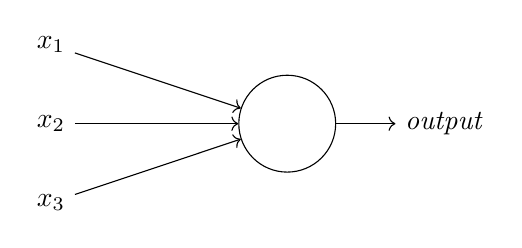
\begin{tikzpicture}[scale=1, transform shape]
\node (a)[circle, draw, minimum width=35pt] at (3, 0) {};
\node (x1)[] at (0, 1) {$x_1$};
\node (x2)[] at (0, 0) {$x_2$};
\node (x3)[] at (0, -1) {$x_3$};
\node (output)[] at (5, 0) {$\mathit{output}$};
\draw[->] (x1) -- (a) ;
\draw[->] (x2) -- (a) ;
\draw[->] (x3) -- (a) ;
\draw[->] (a) -- (output);
\end{tikzpicture}
\caption{An artificial neuron with input $x_1, x_2, x_3$ and one output.}
\label{fig:AN}
\end{figure}

To compute the output we assign to each input a weight, $w_1, \dots, w_n$. The weights represent the importance of the respective inputs to the output. The neuron's output, 0 or 1, is determined by whether the weighted sum $\sum^n_{i=1} w_i x_i$ is less than or greater than  threshold value $t$. Just like the weights, the threshold is a real number which is a parameter of the neuron. To put it in more precise algebraic terms:
\begin{equation}
\mathit{output} = g = \left\{\begin{matrix}
 0 & \text{if } \sum\limits_{i=1}^n w_i x_i < t\\
 1 & \text{if } \sum\limits_{i=1}^n w_i x_i \geq t
\end{matrix}\right.
\label{eq:AF_perceptron}
\end{equation}
This function is also called an \textit{activation function}, in further reading denoted with a $g$.

And that is all we need to create an artificial neuron. As we see in section \ref{sec:neuron_revisted}, the artificial neuron described here is a specific type of artificial neurons called a perceptron. When we understand the perceptron and networks of perceptrons it is easier to understand how other types of neurons work and why they exist.

We can now make an artificial neuron that can act as a logic gate (see figure \ref{fig:neuron_and_gate}, \ref{fig:neuron_or_gate} and \ref{fig:neuron_invert_gate}). By assigning the weights and the threshold we decide on the behaviour.

\begin{figure}[h!]
\centering
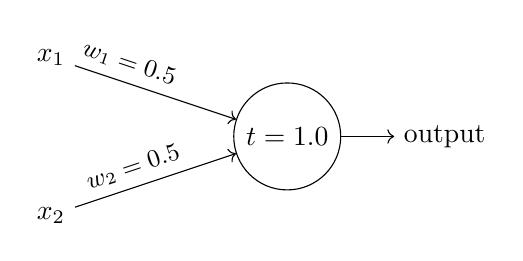
\begin{tikzpicture}[scale=1, transform shape]
\node (a)[circle, draw] at (3, 0) {$t = 1.0$};
\node (x1)[] at (0, 1) {$x_1$};
\node (x2)[] at (0, -1) {$x_2$};
\node (output)[] at (5, 0) {output};
\draw[->] (x1) -- (a) node[pos=0.3,sloped,above] {\small $w_1 = 0.5$};
\draw[->] (x2) -- (a) node[pos=0.4,sloped,above] {\small $w_2 = 0.5$};
\draw[->] (a) -- (output);
\end{tikzpicture}
%\caption{An perceptron given appropriate weights and threshold to act as an AND-gate.}
\caption{Appropriate weights and threshold to act as an AND-gate.}
\label{fig:neuron_and_gate}
\end{figure}
\begin{figure}[h!]
\centering
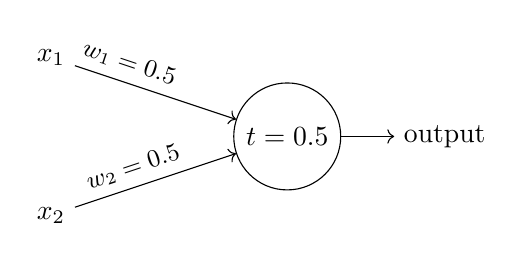
\begin{tikzpicture}[scale=1, transform shape]
\node (a)[circle, draw] at (3, 0) {$t = 0.5$};
\node (x1)[] at (0, 1) {$x_1$};
\node (x2)[] at (0, -1) {$x_2$};
\node (output)[] at (5, 0) {output};
\draw[->] (x1) -- (a) node[pos=0.3,sloped,above] {\small $w_1 = 0.5$};
\draw[->] (x2) -- (a) node[pos=0.4,sloped,above] {\small $w_2 = 0.5$};
\draw[->] (a) -- (output);
\end{tikzpicture}
% \caption{A perceptron given appropriate weights and threshold to act as an OR-gate}
\caption{Appropriate weights and threshold to act as an OR-gate.}
\label{fig:neuron_or_gate}
\end{figure}
\begin{figure}[h!]
\centering
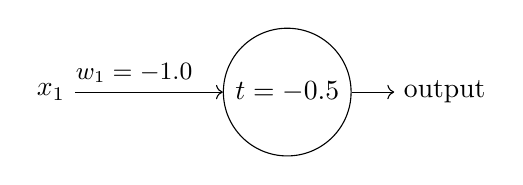
\begin{tikzpicture}[scale=1, transform shape]
\node (a)[circle, draw] at (3, 0) {$t = -0.5$};
\node (x1)[] at (0, 0) {$x_1$};
\node (output)[] at (5, 0) {output};
\draw[->] (x1) -- (a) node[pos=0.4,sloped,above] {\small $w_1 = -1.0$};
\draw[->] (a) -- (output);
\end{tikzpicture}
% \caption{A perceptron given appropriate weights and threshold to act as an INVERT-gate}
\caption{Appropriate weights and threshold to act as an INVERT-gate.}
\label{fig:neuron_invert_gate}
\end{figure}

\noindent
But we are not limited to logic gates. For example, we could make an artificial neuron that decides if we should go to a party. This decision can, of course, be made by weighing the following three factors:
\begin{itemize}
    \item Are your friends going?
    \item Are there cats at the party?
    \item Is the party free?
\end{itemize}
We can represent these three factors by corresponding binary variables $x_1$, $x_2$, and $x_3$. For instance, we'd have $x_1 = 1$ if your friends are going, and $x_1 = 0$ if your friends are not going. Similarly, $x_2=1$ if there are cats at the party, and $x_2=0$ if not. And similarly again for $x_3$ and whether there are entree costs to the party.

Suppose, that your friends make every party the best party possible, so much so that it doesn't matter if you have to pay or that there are no cats; you just have to be there. But if your friends are not there, the party needs to be free and have cats for you to be going. For this decision process we could use an artificial neuron. One way to do this is to choose a weight $w_1=0.6$ for the friends, a $w_2=0.3$ and $w_3=0.2$ for the other conditions and set the threshold $t$ to $0.4$. A larger value for the weight means that the factor matters more in the decision process. This unit can be seen in figure \ref{fig:party_unit}. By varying the weights and the threshold, we can get different models of decision-making. For instance, someone who thinks that cats are better than people (who doesn't?) might have a higher weight for $w_2$ and a lower weight for $w_1$.

\begin{figure}[h!]
\centering
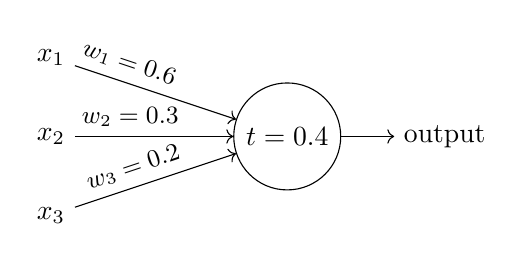
\begin{tikzpicture}[scale=1, transform shape]
\node (a)[circle, draw] at (3, 0) {$t = 0.4$};
\node (x1)[] at (0, 1) {$x_1$};
\node (x2)[] at (0, 0) {$x_2$};
\node (x3)[] at (0, -1) {$x_3$};
\node (output)[] at (5, 0) {output};
\draw[->] (x1) -- (a) node[pos=0.3,sloped,above] {\small $w_1 = 0.6$};
\draw[->] (x2) -- (a) node[pos=0.35,sloped,above] {\small $w_2 = 0.3$};
\draw[->] (x3) -- (a) node[pos=0.4,sloped,above] {\small $w_3 = 0.2$};
\draw[->] (a) -- (output);
\end{tikzpicture}
\caption{A possible perceptron to decide if we should go to a party.}
\label{fig:party_unit}
\end{figure}

\subsection{The limits of perceptrons}
We saw in the figures \ref{fig:neuron_and_gate}, \ref{fig:neuron_or_gate} and \ref{fig:neuron_invert_gate} that perceptrons can represent the simple Boolean functions AND, OR and NOT, but what are the limits to the Boolean functions that can be represented with an artificial neuron? When we look at the activation function in equation \ref{eq:AF_perceptron} we see that it is a linear function. If we would represent our decision making in a two-dimensional plot based on the values of two inputs, then we can only draw one straight line to separate the two decisions. This is shown in figure \ref{fig:linairseperabilty_AND} for an AND-gate. The white and black dots are linear separable. The line between the white and black dots represents the threshold. An artificial neuron can represent an AND-gate. A XOR-gate cannot be represented by an artificial neuron, as there is no single straight line that separates the white and the black dots (see figure \ref{fig:linairseperabilty_EXNOR}).

\begin{figure}
\centering
\begin{tikzpicture}[scale=1, transform shape]

\pgfdeclarelayer{bg}    % declare background layer
\pgfsetlayers{bg,main}  % set the order of the layers (main is the standard layer)

\node (a)[circle, draw, fill=white!30] at (0, 0) {};
\node (a)[circle, draw, fill=white!30] at (2, 0) {};
\node (a)[circle, draw, fill=white!30] at (0, 2) {};
\node (a)[circle, draw, fill=black] at (2, 2) {};

\begin{pgfonlayer}{bg}
\draw[->] (0,-0.5) -- (0,3.5);
\draw[->] (-0.5,0) -- (3.5,0) ;
\draw[-,dashed] (3.5,-0.5) -- (-0.5,3.5) ;
\end{pgfonlayer}
\end{tikzpicture}
\caption{A two-dimensional plot of the decision making for an AND-gate. }
\label{fig:linairseperabilty_AND}
\end{figure}

\begin{figure}
\centering
\begin{tikzpicture}[scale=1, transform shape]

\pgfdeclarelayer{bg}    % declare background layer
\pgfsetlayers{bg,main}  % set the order of the layers (main is the standard layer)

\node (a)[circle, draw, fill=white!30] at (0, 0) {};
\node (a)[circle, draw, fill=black] at (2, 0) {};
\node (a)[circle, draw, fill=black] at (0, 2) {};
\node (a)[circle, draw, fill=white!30] at (2, 2) {};

\begin{pgfonlayer}{bg}
\draw[->] (0,-0.5) -- (0,3.5);
\draw[->] (-0.5,0) -- (3.5,0) ;
%\draw[-] (3.5,-0.5) -- (-0.5,3.5) ;
\end{pgfonlayer}
\end{tikzpicture}
% \caption{A two-dimensional plot of the decision making for a XOR-gate. The white and black dots are not linear separable. An artificial neuron cannot represent an XOR-gate.}
\caption{Plot of decision making for a XOR-gate. The white and black dots are not linear separable.}
\label{fig:linairseperabilty_EXNOR}
\end{figure}

\section{A simple artificial neural network}
A perceptron has it limits in decision making and is in no way close to a complete model for (human) decision making, but, just like logic-gates (see figure \ref{fig:logic_adder}), we can combine them to make more subtle decisions. To get ourselves familiar with the terms used in neural networks we look in this section at the small network depicted in figure \ref{fig:small_perc_network}.

\begin{figure}
\centering
\includegraphics[scale=0.6]{adder}
\caption{An adder built out of NAND-gates.}
\label{fig:logic_adder}
\end{figure}

\begin{figure}
\centering
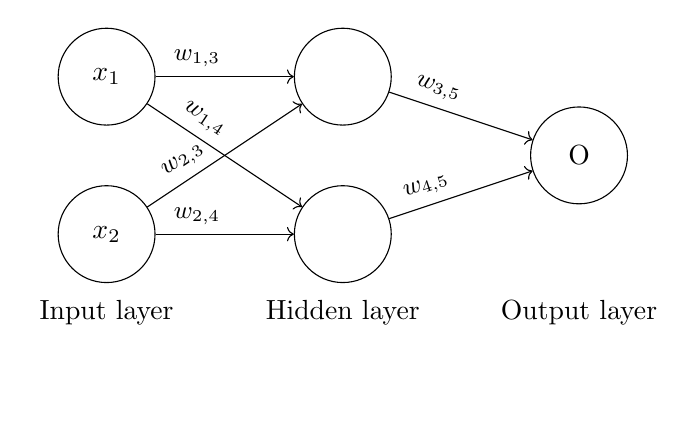
\begin{tikzpicture}[scale=1, transform shape]
\node (x1)[circle, draw, minimum width=35pt] at (0, 1) {$x_1$};
\node (x2)[circle, draw, minimum width=35pt] at (0, -1) {$x_2$};
\node (IL)[circle] at (0, -2) {Input layer};

\node (a)[circle, draw, minimum width=35pt] at (3, 1) {};
\node (b)[circle, draw, minimum width=35pt] at (3, -1) {};
\node (HL)[circle] at (3, -2) {Hidden layer};

\node (c)[circle, draw, minimum width=35pt] at (6, 0) {O};
\node (OL)[circle] at (6, -2) {Output layer};

\draw[->] (x1) -- (a) node[pos=0.3,sloped,above] {\small $w_{1,3}$};
\draw[->] (x1) -- (b) node[pos=0.3,sloped,above] {\small $w_{1,4}$};
\draw[->] (x2) -- (a) node[pos=0.3,sloped,above] {\small $w_{2,3}$};
\draw[->] (x2) -- (b) node[pos=0.3,sloped,above] {\small $w_{2,4}$};

\draw[->] (a) -- (c) node[pos=0.3,sloped,above] {\small $w_{3,5}$};
\draw[->] (b) -- (c) node[pos=0.3,sloped,above] {\small $w_{4,5}$};
\end{tikzpicture}
\caption{A small neural network. Weight $w_{i,j}$ is the weight of the link between unit $i$ and unit $j$.}
\label{fig:small_perc_network}
\end{figure}

\subsection{Units and layers}
Artificial neurons in networks are often called \textit{units}. In a network we can distinguish different type of units. The first layer of units with the input ($x_1$ and $x_2$ in figure \ref{fig:small_perc_network}) are called input units. These units do not get input from other units. Instead their activation depends on external variables (e.g. the grayscale of a pixel). The last layer of units in a network is called the output layer. The activation of the output units in this layer correspondents to the possible answers that we want to get out of the network (e.g., it is a cat). The layers between the input layer and the output layer are called hidden layers. A network without hidden layers is called a single-layer neural network (we do not count the input layer). Neural networks with one or more hidden layers are called multi-layer neural networks.

Layers are connected with each other by links, the connections between two units. As we already discussed, every input has a weight corresponding to it. We could rephrase that to say that every link has a corresponding weight. Where weight $w_{i,j}$ is the weight of the link between unit $i$ and unit $j$.

Note that, although a unit can have multiple outputs arrows, in reality a unit has only one output. Multiple arrows only depict that the output is transferred to multiple units.

\subsection{Feed-forward network}
The network seen in figure \ref{fig:small_perc_network} is a \textit{feed-forward network}. In a feed-forward network the links are unidirectional, and there are no cycles. Technically speaking, a feed-forward network is a directed acyclic graph (DAG). In more layman's terms, in a feed-forward network the activation of the units can only go to the next layer and not back to a previous layer. The significance of the lack of cycles is that computation can proceed uniformly from input units to output units. The activation from the previous time step (the last time the activation of the whole network was calculated) plays no part in the computation, because it is not fed back to an earlier unit. Hence, a feed-forward network simply computes a function of the input values that depends on the weight settings, it has no internal state other than the weights themselves. For instance, the function for the output of the network in figure \ref{fig:small_perc_network} would be:
\begin{equation}
\begin{split}
O & = g(w_{3,5}a_3 + w_{4,5}a_4)\\
       & = g(w_{3,5}g(w_{1,3}a_1 + w_{2,3}a_2) + w_{4,5}g(w_{1,4}a_1 + w_{2,4}a_2))
\end{split}
\end{equation}
where $g$ is the activation function (see section \ref{sec:ArtificialNeuron}), $w_{i,j}$ is the weight of the link between unit $i$ to unit $j$ and $a_i$ is the activation of unit $i$.

A more specific type of a feed-forward network is the \textit{layered feed-forward network}. In a layered feed-forward network each unit is linked only to units in the next layer. There are no links between units in the same layer, no links backward to a previous layer, and no links that skip a layer. The network in figure \ref{fig:small_perc_network} is also a layered feed-forward network.

Neural networks that have cycles and/or bidirectional links are called recurrent networks. Note that our brain is a recurrent network as we otherwise had no short-term memory. In this course, we focus on feed-forward networks because they are relatively well-understood.

\section{Artificial neuron revisited}
\label{sec:neuron_revisted}
The artificial neuron we described before is called a perceptron. There is another type of artificial neuron called a \textit{sigmoid neuron}. In this section we describe the sigmoid neuron, but before we look at the sigmoid neuron let us simplify how we describe perceptrons.

\subsection{Introducing Bias}%\todo{andere titel?}
In section \ref{sec:ArtificialNeuron} we described the working of a perceptron in equation \ref{eq:AF_perceptron} using inputs $x_1 \dots x_n$, corresponding weights $w_1 \dots w_n$ and threshold $t$. The condition $\sum_{i=1}^n w_i x_i > t$ is cumbersome, and we can make two notational changes to simplify it. The first change is to write it as a dot product, $\vec{w} \cdot \vec{x} = \sum_{i=1}^n w_i x_i$, where $\vec{w}$ and $\vec{x}$ are \textit{vectors} whose components are the weights and inputs, respectively. % \footnote{The $\equiv$ means that what is on the left side is equivalent to what is on the right side. In other words, $\vec{w} \cdot \vec{x}$ is the same as $\sum_{i=1}^n w_i x_i$.}

The second change is to move the threshold to the other side of the inequality, and to replace it by what's known as the perceptron's bias: $b = -threshold$. Using the bias instead of the threshold, the perceptron activation function, $g$, can be rewritten:

\begin{equation}
\mathit{output} = g = \left\{\begin{matrix}
 0 & \text{if } \vec{w} \cdot \vec{x} + b < 0\\
 1 & \text{if } \vec{w} \cdot \vec{x} + b \geq 0
\end{matrix} \right.
\label{eq:AF_perceptron_withbias}
\end{equation}

You can think of the bias as a measure of how easy it is to get the perceptron to output a 1. Or to put it in more biological terms, the bias is a measure of how easy it is to get the perceptron to fire. For a perceptron with a really big bias, it's extremely easy for the perceptron to output a 1. But if the bias is very negative, then it's difficult for the perceptron to output a 1.

We can simplify equation \ref{eq:AF_perceptron_withbias} and our calculations a bit more by making the bias a weight of the special input $x_0$ which will always be 1. This will give us the perceptron activation function, $g$,:

\begin{equation}
\mathit{output} = g = \left\{\begin{matrix}
 0 & \text{if } \vec{w} \cdot \vec{x} < 0\\
 1 & \text{if } \vec{w} \cdot \vec{x} \geq 0
\end{matrix}\right.
\label{eq:AF_perceptron_withbiasasweight}
\end{equation}
where $\vec{w}$ is the vector whose components are the weights $w_0 \dots w_n$, $\vec{x}$ is the vector whose components are the inputs $x_0 \dots x_n$, $w_0$ is called the bias weight, with $x_0 = 1$.

This change from threshold to bias simplifies the calculations needed in neural networks, as now only vector multiplications are required. Later, in Section \ref{ch:opencl}, this means that we can more easily offload the neural network calculations to the GPU for training.


\subsection{Sigmoid neuron}
To understand why we have sigmoid neurons and why they are what they are we have to look at what we expect from a learning algorithm for neural networks. Suppose we have a network of perceptrons that we like to learn to solve some problem. For example, the inputs to the network might be the raw pixel data from a scanned, handwritten image of a digit. We would like the network to learn weights such that the output from the network correctly classifies the digit. To see how learning might work, suppose we make a small change in some weight in the network. What we would like is for this small change in weight to cause only a small corresponding change in the output from the network. This property will make learning easier. In figure \ref{fig:small_perc_network_smallChangeInWeights} is schematically depicted what we want.

\begin{figure}
\centering
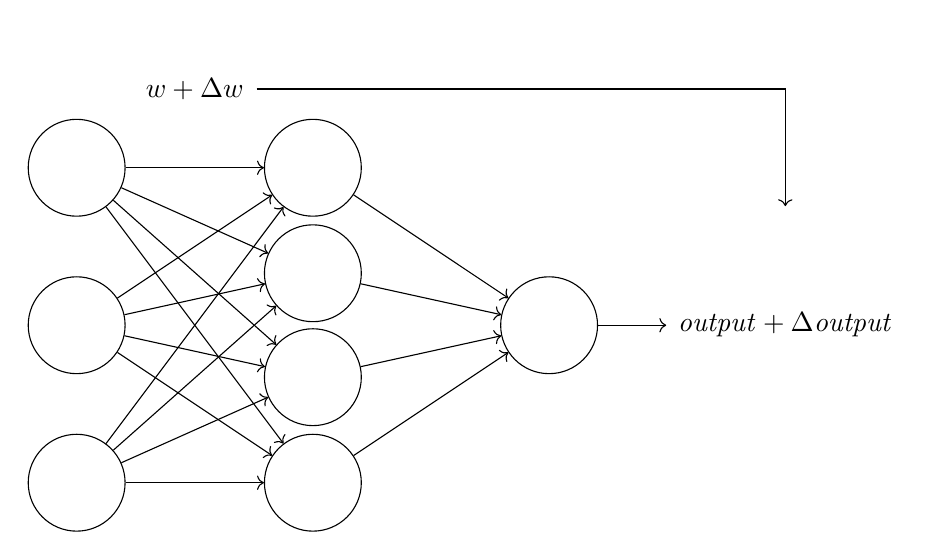
\begin{tikzpicture}[scale=1, transform shape]

\node (x1)[circle, draw, minimum width=35pt] at (0, 2) {};
\node (x2)[circle, draw, minimum width=35pt] at (0, 0) {};
\node (x3)[circle, draw, minimum width=35pt] at (0, -2) {};

\node (w)[circle] at (1.5, 3) {$w + \Delta w$};

\node (a)[circle, draw, minimum width=35pt] at (3, 2) {};
\node (b)[circle, draw, minimum width=35pt] at (3, 0.66) {};
\node (c)[circle, draw, minimum width=35pt] at (3, -0.66) {};
\node (d)[circle, draw, minimum width=35pt] at (3, -2) {};

\node (e)[circle, draw, minimum width=35pt] at (6, 0) {};

\node (output)[circle] at (9, 0) {$\mathit{output} + \Delta \mathit{output}$};

\draw[->] (x1) -- (a) node[pos=0.3,sloped,above] {};
\draw[->] (x1) -- (b) node[pos=0.3,sloped,above] {};
\draw[->] (x1) -- (c) node[pos=0.3,sloped,above] {};
\draw[->] (x1) -- (d) node[pos=0.3,sloped,above] {};
\draw[->] (x2) -- (a) node[pos=0.3,sloped,above] {};
\draw[->] (x2) -- (b) node[pos=0.3,sloped,above] {};
\draw[->] (x2) -- (c) node[pos=0.3,sloped,above] {};
\draw[->] (x2) -- (d) node[pos=0.3,sloped,above] {};
\draw[->] (x3) -- (a) node[pos=0.3,sloped,above] {};
\draw[->] (x3) -- (b) node[pos=0.3,sloped,above] {};
\draw[->] (x3) -- (c) node[pos=0.3,sloped,above] {};
\draw[->] (x3) -- (d) node[pos=0.3,sloped,above] {};


\draw[->] (a) -- (e) node[pos=0.3,sloped,above] {};
\draw[->] (b) -- (e) node[pos=0.3,sloped,above] {};
\draw[->] (c) -- (e) node[pos=0.3,sloped,above] {};
\draw[->] (d) -- (e) node[pos=0.3,sloped,above] {};

\draw[->] (e) -- (output) node[pos=0.3,sloped,above] {};

\draw[->] (w) -| (output) {};

\end{tikzpicture}
\caption{A small neural network. To be able to have an algorithm that can train a neural network, we want a small change in the weights, $w$, results in a small change in the output.}
\label{fig:small_perc_network_smallChangeInWeights}
\end{figure}

If it were true that a small change in a weight causes only a small change in output, then we could use this fact to modify the weights and biases to get our network to behave more in the manner we want. For example, suppose the network was mistakenly classifying an image as an ``8'' when it should be a ``9''. We could figure out how to make a small change in the weights and biases so the network gets a little closer to classifying the image as a ``9''. And then we can repeat this, changing the weights over and over to produce better and better output. The network would be learning.

The problem is that this is not what happens when our network contains perceptrons. In fact, a small change in the weights or bias of any single perceptron in the network can sometimes cause the output of that perceptron to completely flip, say from 0
to 1. That flip may then cause the behaviour of the rest of the network to completely change in some very complicated way. So while a ``9'' might now be classified correctly, the behaviour of the network on all the other images is likely to have completely changed in some hard-to-control way. That makes it difficult to see how to gradually modify the weights and biases so that the network gets closer to the desired behaviour.

We can overcome this problem by introducing a new type of artificial neurons called sigmoid neurons. Sigmoid neurons are similar to perceptrons, but modified such that small changes in their weights and bias cause only a small change in their output. That is the crucial fact which allows a network of sigmoid neurons to learn.

Just like a perceptron, the sigmoid neuron has an input vector $\vec{x}$ and a vector, $\vec{w}$, with weights for each connection. The big difference is that the possible inputs and output of a sigmoid neuron are not only 0's and 1's. The inputs and the output can take any value between 0 and 1. For instance, the value 0.563 is a valid input. To make this also possible for the output the sigmoid neuron uses a different activation function, $g$,:

\begin{equation}
\mathit{output} = g = \sigma(\vec{w} \cdot \vec{x})
\label{eq:AF_sigmoid_withbiasasweight}
\end{equation}
where $\sigma$ is called the \textit{sigmoid function}\footnote{Incidentally, $\sigma$ is sometimes called the logistic function, and this new class of neurons called logistic neurons. It is useful to remember this terminology, since these terms are used by many people working with neural networks. However, we stick with the sigmoid terminology.}, and is defined by:

\begin{equation}
\sigma(z) = \frac{1}{1+e^{-z}}
\label{eq:sigma_function}
\end{equation}

Figure \ref{fig:sigmoid_plot} (left) shows a plot of the sigma function. We can see that it is a smoothed version of the activation function of the perceptron (also called \textit{step-function}, see Figure \ref{fig:sigmoid_plot} (right)). This means that we can represent the same functions as with the perceptrons (such as AND-gates, etc.). Furthermore, we have the desired feature for a learning algorithm: a small change in weights results in a small change in output.

\begin{figure}
\centering
\includegraphics[width=0.45\textwidth]{sigmoid_function_plot}
\hfill
\includegraphics[width=0.45\textwidth]{perceptron_function_plot}
\caption{A plot of the sigmoid function (left) and step-function (right).}
\label{fig:sigmoid_plot}
\end{figure}

% \begin{figure}
% \centering
% \includegraphics[scale=0.5]{perceptron_function_plot}
% \caption{A plot of the activation function of a perceptron.}
% \label{fig:perceptron_plot}
% \end{figure}

\section{Neural networks and learning}
In the previous sections we collected all the parts to create a neural network. To make a learning neural network we only miss two things: examples to learn the task and a learning algorithm. Examples to learn from are called the \textit{training set}. This consists of a set of inputs and the desired outcomes. For instance, in the case of number recognition, a set with images of numbers (input) each with a label of which number it is (desired output). This section explains how a neural network can learn when it has a training set.

\begin{figure}[h!]
\centering
\includegraphics[width=0.8\textwidth, trim={1mm 1mm 1mm 1mm}, clip]{mnistExamples.png}
\caption{A selection of the MNIST training set of handwritten digits.}\label{fig:mnist}
\end{figure}

\subsection{Cost function}
\label{sec:cost_function}
To learn humans need feedback. This is also true for neural networks. The function that tells the neural network how good it is doing is called the \textit{cost function}. There are multiple types of functions than can be used as a cost function. Here, we use the mean squared error (MSE), also known as the quadratic cost function:

\begin{equation}
MSE = \frac{1}{n} \sum_{i=0}^n \left | \vec{y}_i - \vec{a}(\vec{x}_i) \right |^2
\label{eq:MSE}
\end{equation}

The formula for this cost function $C(\vec{w})$ calculates the error (cost $C$) given a vector of weights ($\vec{w}$):\footnote{The math for this cost function might seem complicated, but with a closer look we see it is literally the mean squared error. $\left | \vec{y_i} - \vec{a}(x_i) \right |$ is the difference (or distance) between the output that is given and the output that we want when given input $\vec{x}_i$. In other words $\left | \vec{y}_i - \vec{a}(x_i) \right | $ tells us how wrong the neural network is (i.e. how big the error is) when given input $\vec{x}_i$. As this value can be negative or positive and we are only interested in how wrong the neural network is, we square this value to make all values positive. This is the squared error part of the mean squared error. To get to MSE, we need to calculated the mean. This is done by summing ($\sum$) the squared error over all training inputs and dividing it by the number of training inputs, $i=1,\ldots,n$, ($\frac{1}{2n}$). Actually we also divide by two (hence the 2 in $\frac{1}{2n}$). This has no effect on the functionality when minimising the function, but it makes the function derivative easier. As we use the derivative of this function this  saves us some clutter. In short the MSE is nothing more than the average squared distance between the output of the neural network and the desired output.}

%\note{It is not clear (nor explained) what the $w$ is in $C(w)$. Moreover, we take a range from $1\dots n$, but this is not shown in the RHS of the formula; shouldn't we include an index $i$? And finally, $y$ and $a(x)$ are vectors (values of all output neurons)? If so, for consistency with the rest, they should get a $\vec{ }$.}

\begin{equation}
C(\vec{w}) = \frac{1}{2} MSE = \frac{1}{2n} \sum_{i=0}^n \left | \vec{y}_i - \vec{a}(\vec{x}_i) \right |^2
\label{eq:MSE}
\end{equation}
where $n$ is the number of training inputs, $x$, $\vec{y}_i$ is the desired outcome of the network when $\vec{x}_i$ is the input and $\vec{a}(x_i)$ is the output of the neural network when $\vec{x}_i$ is the input. The notation $\left | \vec{v} \right |$ denotes the usual length function for a vector $\vec{v}$. \footnote{If we have a vector $\vec{v}$ with values $v_1$, $v_2$ and $v_3$, then $\left | v \right |$ is equals to $ \sqrt{{v_1}^2+{v_2}^2+{v_3}^2}$.}

Inspecting the form of the quadratic cost function, we see that $C(\vec{w})$ is non-negative, since every term in the sum is non-negative. Furthermore, the cost $C(\vec{w})$ becomes small, i.e., $C(\vec{w})\approx 0$, precisely when $\vec{y}_i$ is approximately equal to the output, $\vec{a}$, for all training inputs, $\vec{x}_i$. So our training algorithm has done a good job if it can find weights and biases so that $C(\vec{w})\approx0$. By contrast, it's not doing so well when $C(\vec{w})$ is large - that would mean that $\vec{y}_i$ is not close to the output $\vec{a}$ for a large number of inputs. So the aim of our training algorithm will be to minimise the cost $C(\vec{w})$ as a function of the weights and biases. In other words, we want to find a set of weights and biases which make the cost as small as possible\footnote{For some readers the questions might rise why we try to minimise the quadratic cost function, as we just as well could maximise the number of correct classified training samples. The problem with the number of correct classified training samples is that it is not a smooth function. Making a small change in the weights of the units will most of the time result in no change in the number of correct classified training samples. This makes it hard to find which change we should make to the weights of the network. The quadratic cost function is smooth and, therefore, does not have this problem.}.

\subsection{Gradient descent}\label{sec:gradient}
In section \ref{sec:cost_function}, we saw that the goal of a learning algorithm is to minimise the cost function $C(\vec{w})$. As $\vec{w}$ consists out of a lot of weights it takes too much time to calculated for each possible $\vec{w}$ the value of $C(\vec{w})$ to see where $C(\vec{w})$ has the lowest value. A solution for this problem is to use gradient descent. Gradient descent is an optimisation algorithm that approaches a (local) minimum of a function by taking steps in the direction of the negative of the gradient of the function at the current point.

For a first understanding of this algorithm, imagine a blind woman on a mountain that has as goal to go the valley (a minimum). The blind woman doesn't know where she is and can't look around to see which way she has to go. As a solution she feels around to find the slope of the mountain. Now she knows where the mountain goes down and she takes a step in that direction. By repeating this for each step, until she cannot go further down, she knows she ends in a (local) minimum.

Another way to visualise this technique can be seen in figure \ref{fig:valley_with_ball}. The plane is the cost function with weights $v_1$ and $v_2$. A ball is placed at a random place on the plane. The ball is moved a small step into the direction it would roll. This is repeated until we reach the minimum of the plane. When the minimum is reached we have the desired values for $v_1$ and $v_2$.

\begin{figure}
\centering
\includegraphics[scale=0.5]{valley_with_ball}
\caption{Gradient descent can be seen as taking small steps in the direction a ball would roll, until you reach a minimum.}
\label{fig:valley_with_ball}
\end{figure}

Back to our problem. We cannot calculate the minimum of the function, but we can start at a random position (random weights) and then use gradient descent to move down to a minimum. More formal, the algorithm starts with a random $\vec{w}$ and calculates which small change, $\Delta \vec{w}$, reduces $C(\vec{w})$. In other words, we want to find a $\Delta \vec{w}$, that has a negative $\Delta C(\vec{w})$. When $\Delta \vec{w}$ is applied to the weights $C(\vec{w})$ comes closer to a minimum. When we keep repeating this step until we cannot find a $\Delta \vec{w}$, such that $\Delta C(\vec{w})$ is negative, than we are at a (local) minimum and the network has learned its weights.

The $\Delta \vec{w}$ can be found by calculating the gradient on our current position, $\vec{w}$. The gradient can be found by using the derivatives\footnote{If you are not familiar (anymore) with what a derivative is we recommend watching the first 3 chapters of ``essence of calculus'' by 3Blue1Brown that can be found on youtube: \url{https://youtu.be/WUvTyaaNkzM}.} over each weight. The collection of the gradients is called the gradient vector, $\nabla C$:
\begin{equation}
\nabla C = \left (  \frac{\partial C}{\partial w_1}, \dots, \frac{\partial C}{\partial w_n} \right )^T
\end{equation}
where $\frac{\partial C}{\partial w_i}$ is the gradient over weight $w_i$ and note that $T$ here is the transpose operation, turning a row vector into an ordinary (column) vector.

Gradient descent tells us that if we move the weights in the negative direction of $\nabla C$, then we move in the direction of a (local) minimum. With this we can create an update rule that tells us that in each step our new weights, $\vec{w}'$, become:
\begin{equation}
\vec{w}'= \vec{w} - \Delta \vec{w} = \vec{w} - \eta \nabla C
\end{equation}
where $\eta$ is called the learning rate and denotes the size of the step we take in the direction of $-\nabla C$. When $\eta$ is too large we might overshoot a minimum, but a too small $\eta$ requires a lot of steps making the algorithm very slow.

Without vectors, which might make it easier to understand, the update rule for weight $w_i$ is:
\begin{equation}
w_i'= w_i - \Delta w_i = w_i - \eta \frac{\partial C}{\partial w_i}
\end{equation}

\subsection{Single-layer network}
From the last section we know that we can train our neural networks using gradient descent and that we can do that using the derivatives of the cost function. But what are these derivatives? Here we work towards the update rule for our weights for single layer networks. In the next section we generalise this rule to work for multi-layer networks.

First take a look again at the cost function (see equation \ref{eq:MSE}). It requires to look at all training examples for each step. This is a big calculation just for one step. To make our training algorithm faster (but a bit less accurate), we take a step after each training example. The cost function for just one training example is:
\begin{equation}
C = \frac{1}{2} \left | \vec{y} - \vec{a}(\vec{x}) \right |^2
\end{equation}

Now we can use gradient descent to reduce the squared error\footnote{Note that we no longer have to calculate the mean of the squared error, as we are only looking at a single example.} by calculating the partial derivative of $C$ with respect to each weight and updating the weight:
\begin{equation}
\begin{split}
w_i' & = w_i - \eta \frac{\partial C}{\partial w_i} \\
& = w_i - \eta \frac{\partial(\frac{1}{2} \left | \vec{y} - \vec{a}(\vec{x}) \right |^2)}{\partial w_i}
\end{split}
\end{equation}

In a single layer network (see figure \ref{fig:single_layer_neural_network}) each weight has a direct influence on one of the output nodes. The update rule can therefore be rewritten for the weight from input node $j$ to output node $k$:%\todo{Moet dit nog verder uitgewerkt worden?}

\begin{equation}
w_{j,k} = w_{j,k} - \Delta w_{j,k} = w_{j,k} + \eta a_{j} g'(in_k)(y_k - a_k)
\end{equation}
where $a_j$ is the activation of input node $j$, $g'$ is the derivative of the activation function \footnote{For the sigmoid neuron the derivative is given by $g' = g(1-g)$}, $in_k$ is the summed input of output node $k$, $y_k$ is the desired activation of output node $k$ and $a_k$ is the actual activation of output node $k$\footnote{Note the change of sign in the equation: the (partial) derivative $\eta \frac{\partial(\frac{1}{2} \left | \vec{y} - \vec{a}(\vec{x}) \right |^2)}{\partial w_i}$ is negative (as we are looking for the down slope), which means that the sign changes from a minus to a plus.}. This updating rule is called the \textit{delta rule}.

The learning algorithm starts by assigning random values to the weights. Then it keeps updating the weights using the delta rule. Note that the update of the weights happens simultaneously. So, first are all $\Delta w_{j,k}$ calculated and then are all weights updated using the $\Delta w_{j,k}$'s. When a minimum is reached the algorithm stops.

\begin{figure}
\centering
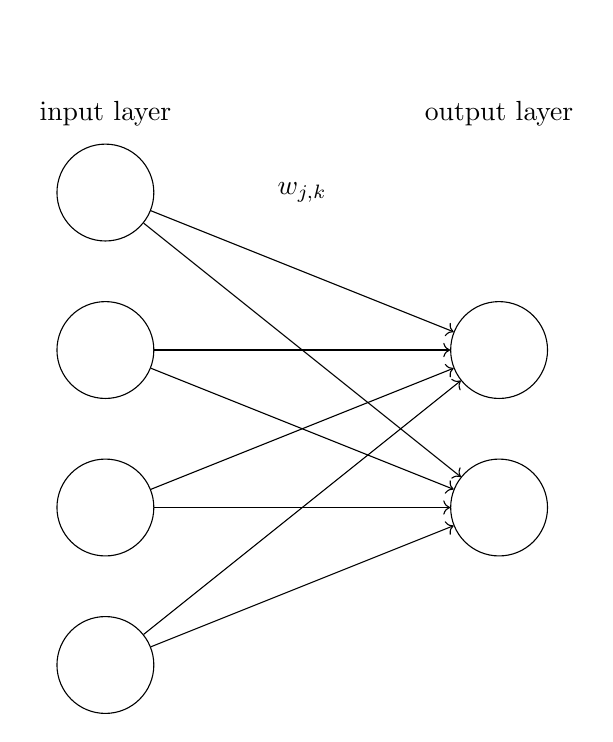
\begin{tikzpicture}[scale=1, transform shape]

\node (input)[circle] at (0, 3) {input layer};

\node (x1)[circle, draw, minimum width=35pt] at (0, 2) {};
\node (x2)[circle, draw, minimum width=35pt] at (0, 0) {};
\node (x3)[circle, draw, minimum width=35pt] at (0, -2) {};
\node (x4)[circle, draw, minimum width=35pt] at (0, -4) {};

\node (output)[circle] at (2.5, 2) {$w_{j,k}$};

\node (output)[circle] at (5, 3) {output layer};
\node (a)[circle, draw, minimum width=35pt] at (5, 0) {};
\node (b)[circle, draw, minimum width=35pt] at (5, -2) {};


\draw[->] (x1) -- (a) node[pos=0.3,sloped,above] {};
\draw[->] (x1) -- (b) node[pos=0.3,sloped,above] {};
\draw[->] (x2) -- (a) node[pos=0.3,sloped,above] {};
\draw[->] (x2) -- (b) node[pos=0.3,sloped,above] {};
\draw[->] (x3) -- (a) node[pos=0.3,sloped,above] {};
\draw[->] (x3) -- (b) node[pos=0.3,sloped,above] {};
\draw[->] (x4) -- (a) node[pos=0.3,sloped,above] {};
\draw[->] (x4) -- (b) node[pos=0.3,sloped,above] {};


\end{tikzpicture}
\caption{A single layer neural network}.
\label{fig:single_layer_neural_network}
\end{figure}

\subsection{Multi-layer network}
In multi-layer networks we have the problem that the weights to hidden layers do not directly influence the output. To  be able to also train these weights we take the idea that hidden node $j$ is ``responsible'' for some fraction of the error in the layer after it. To get to our update rule for the hidden layers we rewrite the delta rule to emphasise what we see as the error:

\begin{equation} \label{eq_output_error}
\Delta_k = g'(in_k)(y_k - a_k)
\end{equation}
\begin{equation}
w_{j,k} = w_{j,k}' + \eta a_j \Delta_k
\end{equation}
where $\Delta_k$ is the error of output node $k$.

If we would know $\Delta_j$, the fraction of error that hidden node $j$ is responsible of in all output nodes, then we can rewrite the update rule to get the update rule for the weights from node $i$ to hidden node $j$:
\begin{equation}
w_{i,j} = w_{i,j}' + \eta a_i \Delta_j
\end{equation}
where $a_i$ is the activation of node $i$. This looks quite similar as the rule for the weights to the output layer. We can calculate $\Delta_j$ with:

\begin{equation} \label{eq:hiddenlayerDeltaerror}
\Delta_j = g'(in_j) \sum_p w_{j,p}\, \Delta_p
\end{equation}
where $w_{j,p}$ is the weight from node $j$ to node $p$ and $\Delta_p$ is the error of node $p$. If node $p$ is an output node then $\Delta_p$ is calculated as $\Delta_k$ in equation \ref{eq_output_error} otherwise it is calculated the same way as $\Delta_j$. In the formula for $\Delta_j$ we see that node $j$ is held ``responsible'' for the error in the nodes it is connected to in the next layer dependent on its activation and its weights.

The algorithm is similar to that of the single-layer networks. The algorithm starts by assigning random values to the weights. Then for each example in the training set it calculates the activation for each node. As the activation of a node depends on the activation of the nodes of the previous layer, this is called forward propagation (the activation moves from the input layer to the output layer). Then the error deltas ($\Delta$) for each node are calculated. As these are dependent on the next layer the delta calculation moves from the output layer to the input layer. The error propagates back through the network. When the deltas are known the weights are updated. One loop over all training samples is called an \textit{epoch}. This is repeated for multiple epochs until some stopping criterion (such as a minimum in the cost function) is reached. This algorithm is called \textit{backpropagation} named after the back propagation of the errors.

\section{Exercises}
\begin{exercise}[NOR-Gate]~\label{ex:NOR-Gate}\\
Determine weights and a threshold for a perceptron that would act as a NOR-gate with three inputs.

%Anwser NOR: $ t = -1$, $w_1 = -2$, $w_2 = -2$ and $w_3 = -2$
\end{exercise}

\begin{exercise}[Neural ADDER]~\label{ex:ADDER}\\
Make an adder out of perceptrons. Draw the network and give the corresponding weights and biases.

%Anwser: \ref{fig:perceptron_adder} all NAND-perceptrons: $ t = -3$, $w_1 = -2$, $w_2 = -2$
\end{exercise}

% \begin{figure}[h!]
% \centering
% \begin{tikzpicture}[scale=0.8, transform shape]
% \node (x1)[circle, draw, minimum width=35pt] at (0, 1) {$x_1$};
% \node (x2)[circle, draw, minimum width=35pt] at (0, -1) {$x_2$};
%
% \node (a)[circle, draw, minimum width=35pt] at (3, 0) {};
%
% \node (b)[circle, draw, minimum width=35pt] at (6, 1) {};
% \node (c)[circle, draw, minimum width=35pt] at (6, -1) {};
% \node (d)[circle, draw, minimum width=35pt] at (6, -3) {};
%
% \node (e)[circle, draw, minimum width=35pt] at (9, 0) {};
%
% \node (sum)[] at (12, 0) {sum: $x_1 \bigoplus x_2$};
% \node (carry)[] at (12, -3) {carry bit: $x_{1} x_{2}$};
%
% \draw[->] (x1) -- (a);
% \draw[->] (x2) -- (a);
%
% \draw[->] (x1) -- (b) ;
% \draw[->] (x2) -- (c) ;
%
% \draw[->] (a) -- (b) ;
% \draw[->] (a) -- (c) ;
% \draw[->, double distance=2pt] (a) -- (d) ; %I don't really like this double line. Solutions? - Jorn
%
% \draw[->] (b) -- (e);
% \draw[->] (c) -- (e);
% \draw[->] (d) -- (carry);
%
% \draw[->] (e) -- (sum);
% \end{tikzpicture}
% \caption{An adder built from perceptrons}.
% \label{fig:perceptron_adder}
% \end{figure}

\begin{exercise}[Programming NNs]~\\
In this exercise you are going to build a (naive) implementation of a neural networks\footnote{In the next section we discuss a ``smarter'', more mathematical, implementation of neural networks.} and use it to classify a number of data sets.

\paragraph{A) Neuron}
Write a class to represent a neuron and its functions. Learning capabilities are not necessary yet. Use this class to implement the neuron of exercise \ref{ex:NOR-Gate} and the network of exercise \ref{ex:ADDER}.

\paragraph{B) Delta Rule}
Add to the neuron class an update function. This function uses the delta rule to updates its weights. The function has as input the desired activation of the node. Test your new function to train the neuron of exercise \ref{ex:NOR-Gate}.

\paragraph{C) Backpropagation}
Add backpropagation to your program. Create the XOR network from the sheets. Initialize the weights with random values. Train the network.

\paragraph{D) Iris dataset}
Create a neural network, using your own code, that is able to classify correctly a high percentage of flowers from the iris dataset\footnote{\url{http://archive.ics.uci.edu/ml/datasets/Iris}}. Make sure you use a train set and a test set.

\noindent
Report the shape of your network and its score on the test set.

\paragraph{E) Weather data [optional]}
Adjust your implementation to work on the weather data from the previous chapter. Can your NN perform as well as (or better than) your $k$-NN implementation?
\end{exercise}

\chapter{Vectorised Neural Networks}\label{ch:opencl}

Though the idea of Neural Networks is older than you might think (refer Chapter \ref{ch:intro}), it is only recently that the techniques started to yield the impressive results that have quickly become synonymous with its name. The reasons for this are myriad, but a large factor was the initial one: the march of technology is catching up with the requirements needed by complex neural networks. To utilise this increase in computing power, various optimisations have been developed for representing neural networks, and an important concept in this is parallelisation. By its very design as a great number of very simple entities, a neural network is a good fit for exploiting modern graphics cards, which consist of hundreds or thousands of cores able to perform a small number of relatively simple tasks. The modern GPU is optimised for matrix and vector calculations, because this is how 3D-graphics are represented. In this chapter we see how neural networks can be represented using basic linear algebra (the area of math concerned with vectors and matrices) to enable us to utilise this vast amount of parallel computing power.

\section{Neural Networks as Matrix-products}\label{sec:nnmp}
We can use the notation and intuitions described above to represent neural networks in a way that can be parallelised. The activation of each layer, whether it is input, output or hidden, is represented by a vector. Weights are represented in matrices, which transform the activation of a layer $a\i L$ to the activation of the next $a^{(L+1)}$ via matrix multiplication. Bias can be represented in multiple ways, but either requires an additional vector or an extra column in each weight-matrix. Gradient descent is used to train the network, like in the object-oriented representation described in Section~\ref{sec:gradient}.

\paragraph{Perceptron}
We start by examining a simple example, a single perceptron:
  \begin{center}
    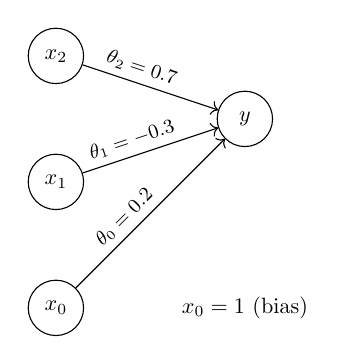
\begin{tikzpicture}[scale=0.8, transform shape]
      \node (x0)[circle, draw, minimum width=25pt] at (0, -2) {$x_0$};
      \node (x1)[circle, draw, minimum width=25pt] at (0, 0) {$x_1$};
      \node (x2)[circle, draw, minimum width=25pt] at (0, 2) {$x_2$};
      \node (y)[circle, draw, minimum width=25pt] at (3, 1) {$y$};
      \node (bias)[] at (3,-2) {$x_0 = 1$ (bias)};
      \draw[->] (x0) -- (y) node[pos=0.4,sloped,above] {\small $\theta_0 = 0.2$};
      \draw[->] (x1) -- (y) node[pos=0.4,sloped,above] {\small $\theta_1 = -0.3$};
      \draw[->] (x2) -- (y) node[pos=0.4,sloped,above] {\small $\theta_2 = 0.7$};
    \end{tikzpicture}
  \end{center}

Instead of considering each input $x_n$ and each weight $\theta_n$ as a separate value, we store them in two vectors $\vec x$ and $\vec\theta$. Normally, we use the matrix $\Theta$ to store the weights between two layers, where each column matches a node in the domain ($a\i L$, the input of the transformation) and each row matches a node in the co-domain ($a^{(L+1)}$, the output of the transformation). In this case, we have a single node in the co-domain, so the weight-matrix consists of a single row: a vector.

By taking the inner product of the input vector $\vec x$ and the weight vector $\vec \theta$, we can use a single operation to multiply each input value with its associated weight, and sum the result. So $y = \sigma(\theta_1x_1 + \theta_2x_2)$ becomes $y = \sigma\inprod{\theta}{x}$\footnote{Remember, $\sigma$ represents the \textit{sigmoid activation function}, as introduced in Section \ref{sec:neuron_revisted}.}.

Note that the bias is, in this case, added as a column to the weight matrix (or rather, in this simple example, a single value added to the weight matrix). This value is typically added as column $0$, which in this vector example means $\theta_0$. Furthermore, each input and activation layer is prepended\footnote{So, $\begin{bmatrix}x_1 & x_2\end{bmatrix}$ becomes $\begin{bmatrix}1 & x_1 & x_2\end{bmatrix} $. We can write this as $\vec a \leftarrow \begin{bmatrix}1 & \vec a\end{bmatrix}$.} with a $0$-index element, which will alway be $1$ (as $1 \times \theta_0 = \theta_0$, the bias). Thus, the expansion of our inner product including the bias is $y = \sigma(\theta_0x_0 + \theta_1x_1 + \theta_2x_2)$. In a later example, we will see another way to represent the bias using a separate vector.

\paragraph{Hidden Layer}
We now consider a more complicated network, by adding a single hidden layer consisting of $4$ neurons.

  \vspace{3mm}
  \begin{center}
    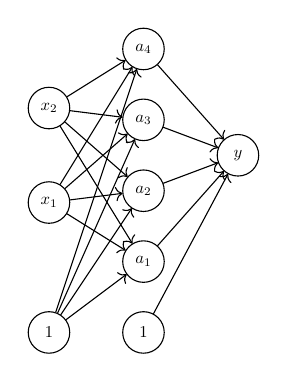
\begin{tikzpicture}[scale=0.6, transform shape]
      \node (x0)[circle, draw, minimum width=25pt] at (0, -3.75) {$1$};
      \node (x1)[circle, draw, minimum width=25pt] at (0, -1) {$x_1$};
      \node (x2)[circle, draw, minimum width=25pt] at (0, 1) {$x_2$};
      \node (a1)[circle, draw, minimum width=25pt] at (2, -2.25) {$a_1$};
      \node (a2)[circle, draw, minimum width=25pt] at (2, -0.75) {$a_2$};
      \node (a3)[circle, draw, minimum width=25pt] at (2, 0.75) {$a_3$};
      \node (a4)[circle, draw, minimum width=25pt] at (2, 2.25) {$a_4$};
      \node (a0)[circle, draw, minimum width=25pt] at (2, -3.75) {$1$};
      \node (y)[circle, draw, minimum width=25pt] at (4, 0) {$y$};
      \draw[->] (x0) -- (a1) [] {};
      \draw[->] (x0) -- (a2) [] {};
      \draw[->] (x0) -- (a3) [] {};
      \draw[->] (x0) -- (a4) [] {};
      \draw[->] (x1) -- (a1) [] {};
      \draw[->] (x1) -- (a2) [] {};
      \draw[->] (x1) -- (a3) [] {};
      \draw[->] (x1) -- (a4) [] {};
      \draw[->] (x2) -- (a1) [] {};
      \draw[->] (x2) -- (a2) [] {};
      \draw[->] (x2) -- (a3) [] {};
      \draw[->] (x2) -- (a4) [] {};
      \draw[->] (a1) -- (y) [] {};
      \draw[->] (a2) -- (y) [] {};
      \draw[->] (a3) -- (y) [] {};
      \draw[->] (a4) -- (y) [] {};
      \draw[->] (a0) -- (y) [] {};
    \end{tikzpicture}
\end{center}

We can calculate $a_1$ as $\inprod{x}{{\theta\i1}}$, $a_2$ as $\inprod{x}{{\theta\i2}}$, et cetera. But, as we have seen, we can do an entire series of inner products as a single operation using the matrix product. Multiplying $A\vec b =c$, each element $\vec c_y$ in $\vec c$ is calculated by $\inprod{A_{x,*}}{\vec b_y}$. We can use this to our advantage, and stack every weight vector $\vec{\theta\i n}$ for every neuron $a_n$ into a weight matrix $\Theta$. Multiplying this with our input vector $\vec x$ results in a new vector $\vec a$, consisting of all activation values in the succeeding layer.

$$\Theta\i1 = \begin{bmatrix}- & \vec{\theta^1} & - \\ - & \vec{\theta^2} & - \\ - & \vec{\theta^3} & - \\ - & \vec{\theta^4} & -\end{bmatrix}, \quad \vec{a} = \sigma(\Theta\i1\vec{x})$$

The entire picture now looks like this:

  \begin{minipage}{0.3\textwidth} \begin{center}
    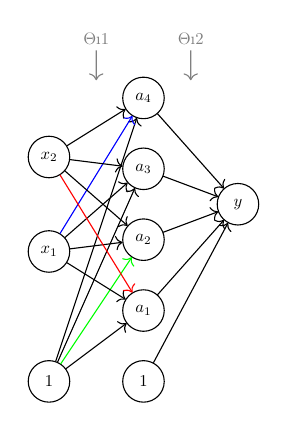
\begin{tikzpicture}[scale=0.6, transform shape]
      \node (l1)[] at (1,3.5) {\color{gray} $\Theta\i1$};
      \node (l2)[] at (3,3.5) {\color{gray} $\Theta\i2$};
      \node (t1)[] at (1,2.5) {};
      \node (t2)[] at (3,2.5) {};
      \draw[gray, ->] (l1) -- (t1) [] {};
      \draw[gray, ->] (l2) -- (t2) [] {};
      \node (x0)[circle, draw, minimum width=25pt] at (0, -3.75) {$1$};
      \node (x1)[circle, draw, minimum width=25pt] at (0, -1) {$x_1$};
      \node (x2)[circle, draw, minimum width=25pt] at (0, 1) {$x_2$};
      \node (a1)[circle, draw, minimum width=25pt] at (2, -2.25) {$a_1$};
      \node (a2)[circle, draw, minimum width=25pt] at (2, -0.75) {$a_2$};
      \node (a3)[circle, draw, minimum width=25pt] at (2, 0.75) {$a_3$};
      \node (a4)[circle, draw, minimum width=25pt] at (2, 2.25) {$a_4$};
      \node (a0)[circle, draw, minimum width=25pt] at (2, -3.75) {$1$};
      \node (y)[circle, draw, minimum width=25pt] at (4, 0) {$y$};
      \draw[->] (x0) -- (a1) [] {};
      \draw[green, ->] (x0) -- (a2) [] {};
      \draw[->] (x0) -- (a3) [] {};
      \draw[->] (x0) -- (a4) [] {};
      \draw[->] (x1) -- (a1) [] {};
      \draw[->] (x1) -- (a2) [] {};
      \draw[->] (x1) -- (a3) [] {};
      \draw[blue, ->] (x1) -- (a4) [] {};
      \draw[red, ->] (x2) -- (a1) [] {};
      \draw[->] (x2) -- (a2) [] {};
      \draw[->] (x2) -- (a3) [] {};
      \draw[->] (x2) -- (a4) [] {};
      \draw[->] (a1) -- (y) [] {};
      \draw[->] (a2) -- (y) [] {};
      \draw[->] (a3) -- (y) [] {};
      \draw[->] (a4) -- (y) [] {};
      \draw[->] (a0) -- (y) [] {};
    \end{tikzpicture}
  \end{center} \end{minipage}\begin{minipage}{0.7\textwidth}
    $$\Theta\i1 = \begin{bmatrix}0.1 & -0.2 & \color{red} -0.3 \\ \color{green} 0.4 & -0.5 & 0.6 \\ -0.7 & 0.8 & 0.9 \\ -0.1 & \color{blue}0.2 & 0.3\end{bmatrix}$$ $$\Theta\i2 = \begin{bmatrix}0.1 & 0.1 & 0.2 & 0.3 & 0.5\end{bmatrix}$$
  \end{minipage}\mbox{}\\[4mm]

    Each value in $\Theta\i 1$ matches a weight between the input and hidden layer; $\Theta\i1_{ij}$ represents the weight from $x_j$ to $a_i$. In this case, rows count from $1$, columns count from $0$ with column $0$ representing the bias. Each value in $\Theta\i 2$ matches a weight between the hidden layer and the output. In this case, it could have been represented by a vector because the output value $y$ is a scalar, but to avoid mixing and matching lowercase and uppercase Greek letters we keep every weight a matrix for now. Calculating $y$ from $\vec x$, $\Theta\i 1$, and $\Theta\i 2$ looks like this:

  $$\vec{a} = \sigma(\Theta\i1\vec{x}), \quad \vec{a^\prime} = \begin{bmatrix} 1 & \vec{a}\end{bmatrix}, \quad y = \sigma(\Theta\i2\vec{a^\prime})$$

  $$y = \sigma(\Theta\i2\vec{\begin{bmatrix} 1 & \sigma(\Theta\i1\vec{x})\end{bmatrix}})$$

\paragraph{Bias}
  So far, we have been representing the bias for each layer using an extra weight, which gets multiplied by $1$ for each neuron in the layer. An alternative way of representing the bias is as a separate vector, to be added after the matrix multiplication. Using the same sample as above, we can also represent the network as shown below. This time, both rows and columns count from 1 as there is no bias column $0$.

  \begin{minipage}{0.4\textwidth} \begin{center}
    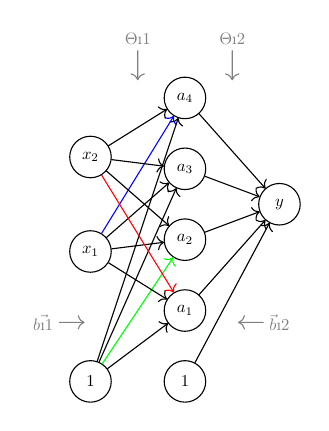
\begin{tikzpicture}[scale=0.6, transform shape]
      \node (l1)[] at (1,3.5) {\color{gray} $\Theta\i1$};
      \node (l2)[] at (3,3.5) {\color{gray} $\Theta\i2$};
      \node (l3)[] at (-1, -2.5) {\color{gray} $\vec{b\i1}$};
      \node (l4)[] at (4, -2.5) {\color{gray} $\vec b\i2$};
      \node (t1)[] at (1,2.5) {};
      \node (t2)[] at (3,2.5) {};
      \node (t3)[] at (0,-2.5) {};
      \node (t4)[] at (3,-2.5) {};
      \draw[gray, ->] (l1) -- (t1) [] {};
      \draw[gray, ->] (l2) -- (t2) [] {};
      \draw[gray, ->] (l3) -- (t3) [] {};
      \draw[gray, ->] (l4) -- (t4) [] {};
      \node (x0)[circle, draw, minimum width=25pt] at (0, -3.75) {$1$};
      \node (x1)[circle, draw, minimum width=25pt] at (0, -1) {$x_1$};
      \node (x2)[circle, draw, minimum width=25pt] at (0, 1) {$x_2$};
      \node (a1)[circle, draw, minimum width=25pt] at (2, -2.25) {$a_1$};
      \node (a2)[circle, draw, minimum width=25pt] at (2, -0.75) {$a_2$};
      \node (a3)[circle, draw, minimum width=25pt] at (2, 0.75) {$a_3$};
      \node (a4)[circle, draw, minimum width=25pt] at (2, 2.25) {$a_4$};
      \node (a0)[circle, draw, minimum width=25pt] at (2, -3.75) {$1$};
      \node (y)[circle, draw, minimum width=25pt] at (4, 0) {$y$};
      \draw[->] (x0) -- (a1) [] {};
      \draw[green, ->] (x0) -- (a2) [] {};
      \draw[->] (x0) -- (a3) [] {};
      \draw[->] (x0) -- (a4) [] {};
      \draw[->] (x1) -- (a1) [] {};
      \draw[->] (x1) -- (a2) [] {};
      \draw[->] (x1) -- (a3) [] {};
      \draw[blue, ->] (x1) -- (a4) [] {};
      \draw[red, ->] (x2) -- (a1) [] {};
      \draw[->] (x2) -- (a2) [] {};
      \draw[->] (x2) -- (a3) [] {};
      \draw[->] (x2) -- (a4) [] {};
      \draw[->] (a1) -- (y) [] {};
      \draw[->] (a2) -- (y) [] {};
      \draw[->] (a3) -- (y) [] {};
      \draw[->] (a4) -- (y) [] {};
      \draw[->] (a0) -- (y) [] {};
    \end{tikzpicture}
  \end{center} \end{minipage}\hspace{1mm}\begin{minipage}{0.55\textwidth} \small
    $$\Theta\i1 = \begin{bmatrix} -0.2 & \color{red} -0.3 \\ -0.5 & 0.6 \\ 0.8 & 0.9 \\ \color{blue}0.2 & 0.3\end{bmatrix},
    \vec{b\i1} = \begin{bmatrix}0.1 \\ \color{green} 0.4 \\ -0.7 \\ -0.1\end{bmatrix}$$\\
      $$\Theta\i2 = \begin{bmatrix}0.1 & 0.2 & 0.3 & 0.5\end{bmatrix}, \quad \vec b^{(2)} = \begin{bmatrix}0.1 \end{bmatrix}$$
  \end{minipage}\mbox{}\\[4mm]
  $$\vec{a} = \sigma(\Theta\i1\vec{x} + \vec{b\i1}), \quad y = \sigma(\Theta\i2\vec{a}+\vec b\i2)$$

  $$y = \sigma(\Theta\i2\sigma(\Theta\i1\vec{x} + \vec{b\i1})+\vec b\i2)$$\\[-4mm]

  Notice that we have written $\vec b\i 2$ as a $1$-element vector instead of a scalar, just as we write the single row matrix $\Theta\i 2$ as a matrix instead of a vector.\\

\begin{exercise}[Bias Representation]\mbox{}\\
  Confirm the equivalence of both bias representations by calculating the results in both instances.\\
  \textbf{Bonus:} Prove both bias representations are the same.
\end{exercise}

\def\Item#1#2{\item\makebox[3.5cm]{#1\hfill} \quad #2}

\subsection{Going Deeper}\label{sec:deeper}
Now, consider a more complex example:
  \begin{itemize}
    \item 2 hidden layers
    \item 1024 input neurons
    \item 42 in hidden layer 1
    \item 28 in hidden layer 2
    \item 12 output neurons
  \end{itemize}

To represent this, we need the following vectors:

  \begin{itemize}
      \Item{input vector}{$\vec{x} \in \mathbb{R}^{1024}$}
      \Item{activation vector HL1}{$\vec{a\i1} \in \mathbb{R}^{42}$}
      \Item{activation vector HL2}{$\vec{a\i2} \in \mathbb{R}^{28}$}
      \Item{output vector}{$\vec{y} \in \mathbb{R}^{12}$}
  \end{itemize}

Which gives us the following weights and equalities:
  $$\Theta\i1 \in \mathbb{R}^{42 \times 1024+1}, \Theta\i2 \in \mathbb{R}^{28 \times 42+1}, \Theta\i3 \in \mathbb{R}^{12 \times 28+1}$$
  $$\vec{a\i1} = \sigma(\Theta\i1\begin{bmatrix} 1 & \vec{x}\end{bmatrix})$$
  $$\vec{a\i2} = \sigma(\Theta\i2\begin{bmatrix} 1 & \vec{a\i1}\end{bmatrix}) = \sigma(\Theta\i2\begin{bmatrix} 1 & \sigma(\Theta\i1\begin{bmatrix} 1 & \vec{x}\end{bmatrix})\end{bmatrix})$$
  $$\vec{y} = \sigma(\Theta\i3\begin{bmatrix} 1 & \vec{a\i2}\end{bmatrix}) = \sigma(\Theta\i3\begin{bmatrix} 1 & \sigma(\Theta\i2\begin{bmatrix} 1 & \sigma(\Theta\i1\begin{bmatrix} 1 & \vec{x}\end{bmatrix})\end{bmatrix})\end{bmatrix})$$\\[-3mm]

Or, with bias as a separate vector:
  $$\Theta\i1 \in \mathbb{R}^{42 \times 1024}, \Theta\i2 \in \mathbb{R}^{28 \times 42}, \Theta\i3 \in \mathbb{R}^{12 \times 28}$$
  $$\vec{b\i1} \in \mathbb{R}^{42}, \vec{b\i2} \in \mathbb{R}^{28}, \vec{b\i3} \in \mathbb{R}^{12}$$
  $$\vec{a\i1} = \sigma(\Theta\i1\vec{x}+\vec{b\i1})$$
  $$\vec{a\i2} = \sigma(\Theta\i2\vec{a\i1}+\vec{b\i2}) = \sigma(\Theta\i2\sigma(\Theta\i1\vec{x}+\vec{b\i1})+\vec{b\i2})$$
  $$\vec{y} = \sigma(\Theta\i3\vec{a\i2}+\vec{b\i3}) = \sigma(\Theta\i3\sigma(\Theta\i2\sigma(\Theta\i1\vec{x}+\vec{b\i1})+\vec{b\i2})+\vec{b\i3})$$

\begin{exercise}[Another Deep Neural Network]\mbox{}\\
  Consider a network consisting of the following:
  \begin{itemize}
    \item 3 hidden layers
    \item 576 input neurons
    \item 64 neurons in hidden layer 1
    \item 16 neurons in hidden layer 2
    \item 16 neurons in hidden layer 3
    \item 4 output neurons
  \end{itemize}
  Which matrices do we need to implement this, and what are their dimensions? How is the output-vector $\vec y$ defined in terms of $\vec x$? Write the math out as we have seen above, both for bias-as-column and bias-as-vector representations.
\end{exercise}

\subsection{Vectorised Cost Function}
Like most forms of supervised machine learning, the cost-function is based on the difference between the output of the network and the expected answer. For each training example, we need to compare two vectors: the predicted answer $\vec y$ and the correct answer $\vec{y^\prime}$. Here, we use the sum of squared errors, $J = (\vec{y}_{1} - \vec{y^\prime}_{1})^2 + (\vec{y}_{2} - \vec{y^\prime}_{2})^2 + \dots + (\vec{y}_{n} - \vec{y^\prime}_{n})^2$. If, for increased clarity, we define an error vector $\vec e = \vec y - \vec {y^\prime}$, we can write this as $J = \vec e_1\vec e_1+\vec e_2\vec e_2 + \dots + \vec e_n \vec e_n$. We have seen this pattern before: what we have here is the inner product of $\vec{e}$ and itself. Vectorised, we can thus write our cost function as $J = \inprod{e}{e} = \vec e^2$. Substituting our original difference between $\vec y$ and $\vec {y^\prime}$ back for $\vec e$ yields $J = \bra{\vec{y}-\vec{y^\prime}}\ket{\vec{y}-\vec{y^\prime}} \quad \text{or} \quad J = (\vec{y}_{} - \vec{y^\prime}_{})^2$.

\subsection{Further Parallelisation}
  Up until now, we have represented each layer in our neural network as a vector, and used matrices to map between each. Each vector $\vec x$ represents a single input vector, associated with a single output vector $\vec y$. We can evaluate multiple examples in parallel by replacing our vectors by matrices. As an intermediate step, consider our deep example from Section~\ref{sec:deeper}, but this time, interpret each $n$-vector as if it where a $1 \times n$ matrix (for the sake of saving trees, we will only consider the bias-as-vector representation, but the same holds for bias-as-column).

  $$X \in \mathbb{R}^{1024\times 1}, A\i1 \in \mathbb{R}^{42\times 1}, A\i2 \in \mathbb{R}^{28\times 1}, Y \in \mathbb{R}^{12\times 1}$$\\[-3mm]
  $$\Theta\i1 \in \mathbb{R}^{42 \times 1024}, \Theta\i2 \in \mathbb{R}^{28 \times 42}, \Theta\i3 \in \mathbb{R}^{12 \times 28}$$
  $$B\i1 \in \mathbb{R}^{42 \times 1}, B\i2 \in \mathbb{R}^{28 \times 1}, B\i3 \in \mathbb{R}^{12 \times 1}$$\\[-2mm]
  $$A\i1 = \sigma(\Theta\i1X+B\i1)$$
  $$A\i2 = \sigma(\Theta\i2A\i1+B\i2)$$
  $$Y = \sigma(\Theta\i3A\i2+B\i3)$$

  \begin{exercise}[Vectors to Matrices]\mbox{}\\
    Verify that the example given above is equivalent to the vector-based example from Section~\ref{sec:deeper}.
  \end{exercise}

We can add as many columns as we need to accomodate the number of training examples that we want to process in parallel. In general, to evaluate $n$ examples at a time, we need the following dimensions for our $\Theta$ and $B$ matrices:

  $$X \in \mathbb{R}^{1024\times n}, A\i1 \in \mathbb{R}^{42\times n}, A\i2 \in \mathbb{R}^{28\times n}, Y \in \mathbb{R}^{12\times n}$$
  $$B\i1 \in \mathbb{R}^{42 \times n}, B\i2 \in \mathbb{R}^{28 \times n}, B\i3 \in \mathbb{R}^{12 \times n}$$\\[-2mm]

\section{Learning}
Now that we know how to represent our network, we can look towards learning. Like in the object-oriented representation from Section~\ref{sec:gradient}, we can use Gradient Descent. We can use multivariable calculus to find the gradient $\nabla J$ of our cost function, and move our weights and biasses accordingly. Tweaking this for a lot of variables quickly gets complicated, which is why we use the functions available to us in NumPy to avoid having to do this ourselves, which is generally error-prone. To get a feel of what is happening, take a look at the videos made by 3Blue1Brown\footnote{A playlist with the neural network series by 3Blue1Brown is available at \url{https://youtu.be/aircAruvnKk}.} animating this process.

\begin{exercise}[Gradient Descent]\mbox{}\\
  Watch the following videos on YouTube, and explain in your own words what the algorithm does.
  \begin{itemize}
    \item \href{https://www.youtube.com/watch?v=aircAruvnKk}{But what *is* a Neural network?}
    \item \href{https://www.youtube.com/watch?v=IHZwWFHWa-w}{Gradient descent, how neural networks learn} (optional)
    \item \href{https://www.youtube.com/watch?v=Ilg3gGewQ5U}{What is backpropagation and what is it actually doing?}
    \item \href{https://www.youtube.com/watch?v=tIeHLnjs5U8}{Backpropagation calculus} (optional)
  \end{itemize}
\end{exercise}

\section{Implementation using NumPy}
We now turn our attention towards implementing what we have learned using NumPy. NumPy is a package which provides a large array of fundamental mathemathical functions and structures to Python. Even more bare-metal approaches exist for maximising GPU perfomance, such as OpenCL\footnote{\url{https://www.khronos.org/opencl}} and CUDA\footnote{\url{https://developer.nvidia.com/cuda-zone}}. In this course, we focus on NumPy, which provides a nice middle ground between readability and performance.

\subsection{Vectors}
Vectors are represented as numpy arrays. A numpy array can be generated from a regular array using \py|numpy.array(regular_array)|, e.g. \py|numpy.array([1,2,3])|. The \py|numpy.array| function is idempotent: calling it on an existing numpy array results an unchanged array. This is useful when writing functions to ensure a parameter is a numpy array, as it allows one to convert the paramater regardless of whether it was already a Numpy array.

Numpy arrays support vector addition and scalar multiplication using overloaded versions of the regular \py|+| and \py|*| operators. For the inner product, the \py|dot| function is used: \py|numpy.dot(u,v)| can be used to calculate $\inprod{u}{v}$.

Note that $\inprod{u}{v}$ is an entirely different operation from Python's \py|u*v|, which calculates the Hadamard product (see Aside \ref{hadamard}), which is different from the inner product. Furthermore, it is possible to add a scalar to a vector, which results in the scalar being \emph{broadcasted} into a vector:
$$\begin{bmatrix}1\\2\\3\end{bmatrix} + 1 = \begin{bmatrix}1\\2\\3\end{bmatrix}+\begin{bmatrix}1\\1\\1\end{bmatrix} = \begin{bmatrix}2\\3\\4\end{bmatrix}$$
  Broadcasting will be explained in more detail in Section \ref{broad}, after we have familiarised ourselves with numpy's notation for matrices.

\begin{aside}[The Hadamard Product]\mbox{}\\\label{hadamard}
The Hadamard product $\odot : V \times V \to V$ of two vectors, also referred to as pointwise multiplication, is defined as follows:
$$ \vec u \odot \vec v = \begin{bmatrix} \vec u_1 \vec v_1 \\ \vec u_2 \vec v_2 \\ \vdots \\ \vec u_n \vec v_n \end{bmatrix} $$

Notice that this means that the Hadamard product of two vectors in space $\mathbb{R}^n$ will always be another vector in $\mathbb{R}^n$. This matches the type Python expects of the \py|*| function, which is likely why this product was chosen despite being a less common operation than the inner product. This behaviour is also consistent with the broadcasting described below.
\end{aside}

\subsection{Matrices}
Matrices can be generated in numpy using the same \py|numpy.array| function as vectors, only using nested arrays: \py|numpy.array([[1,2,3],[2,3,4]])| represents the $2\times 3$ matrix below:

$$\begin{bmatrix}1&2&3\\2&3&4\end{bmatrix}$$

  Matrices addition and scalar multiplication work the same way as for vectors, as does the Hadamard product, broadcasting if necessary. The same \py|dot| function used for the inner product is also used for matrix multiplication.

\subsection{Broadcasting}\label{broad}
  Broadcasting can occur whenever Python expects two operands to be of equal dimension. If this expectation is met, everything will proceed as normal. Otherwise, Python will attempt to correct the situation by expanding the smaller operand. This can only occur when one dimension of the operand is equal to $1$, in which case Python repeats what it knows in order to correct the size of the operand. Thus, it is possible to add a scalar to a vector, or add a vector to a matrix:
  $$\begin{bmatrix}1\\2\\3\end{bmatrix} + \begin{bmatrix}1&1&1\\1&1&1\\  1&1&1\\ \end{bmatrix} = \begin{bmatrix}2&2&2\\3&3&3\\4&4&4\\ \end{bmatrix}$$

When making use of broadcasting, keep in mind that a numpy array by default is interpreted as a row vector. It is possible to explicitly create row and column vectors, as shown in the following examples. This is useful for controlling broadcasting, or when for example an outer product is desired.
Compare:
\begin{lstlisting}
    numpy.array([1,2,3]) # Vector
  + numpy.array([[1,1,1],[1,1,1],[1,1,1]])
 #= numpy.array([[2,3,4],[2,3,4],[2,3,4]])
\end{lstlisting}
\begin{lstlisting}
    numpy.array([[1,2,3]]) # Explicit Row Vector
  + numpy.array([[1,1,1],[1,1,1],[1,1,1]])
 #= numpy.array([[2,3,4],[2,3,4],[2,3,4]])
\end{lstlisting}
\begin{lstlisting}
    numpy.array([[[1],[2],[3]]]) # Explicit Column Vector
  + numpy.array([[1,1,1],[1,1,1],[1,1,1]])
 #= numpy.array([[2,2,2],[3,3,3],[4,4,4]])
\end{lstlisting}

Notice that only the third example corresponds to the addition using a column vector shown above.
%It is also possible to explicitly create a row vector by using \py|numpy.array([[1],[2],[3]])

\subsection{Example: Perceptron}
We can now return to our first example (Section \ref{sec:nnmp}): the simple perceptron. We encode $\vec x$ and $\vec \theta$ as numpy \py|array|s, and take their inner product to determine $y$. Using $0.2$ and $0.3$ for the input values of $\vec x$, we get the following:

\begin{lstlisting}
  def sigmoid(x): # Also available from SciKit
      return 1 / (1 + math.e ** (-x))

  x = numpy.array([1,0.2,0.3]) # Bias and two input values
  theta = numpy.array([0.2,-0.3,0.7])
  y = sigmoid(numpy.dot(theta, x)) # 0.5866175789173301
  # alternative:
  # y = sigmoid(theta.dot(x))
\end{lstlisting}

\subsection{Hidden Layers}
Moving on to our more complex example featuring a hidden layer, we can expand upon this. Remember that we have seen two ways to encode the bias: bias-as-column and bias-as-vector. This difference must be taken into account when translating our example into code.

Thanks to broadcasting, our sigmoid function will work on numpy arrays without change. For more complex functions (e.g. the $tanh$ or $tan^{-1}$ activation function), it is possible to create a vectorised version of said function by using Numpy's \py|vectorise| function. This creates a new function that will map its input function over an array.

\begin{lstlisting}
  from math import tanh

  vectorised_activation = numpy.vectorise(tanh)
\end{lstlisting}

\paragraph{Bias-as-column}
For this representation, we need to introduce one final bit of notation: prepending the bias to an activation layer: $\vec{a^\prime} = \begin{bmatrix} 1 & \vec{a}\end{bmatrix}$. In Numpy, we can use the \py|append| function for this: \py|numpy.append(1, a)|. The resulting code looks as follows:

\begin{lstlisting}
  x = numpy.array([1,0.2,0.3]) # Bias and two input values
  Theta1 = numpy.array([[0.1,-0.2,-0.3]
                       ,[0.4,-0.5,0.6]
                       ,[-0.7,0.8,0.9]
                       ,[-0.1,0.2,0.3]])
  a = vectorised_sigmoid(numpy.dot(Theta1, x))
  # a = [ 0.49250056,  0.61774787,  0.4329071 ,  0.50749944]
  a_prime = numpy.append(1, a) # Add bias
  Theta2 = numpy.array([[0.1,0.1,0.2,0.3,0.5]])
  y = vectorised_sigmoid(numpy.dot(Theta2, a_prime))
  # y = 0.65845607
\end{lstlisting}
\paragraph{Bias-as-vector}
In this representation, we do not need to \py|append| anything; rather, we need some additional values:
\begin{lstlisting}
  x = numpy.array([0.2,0.3]) # Just two input values
  Theta1 = numpy.array([[-0.2,-0.3]
                       ,[-0.5,0.6]
                       ,[0.8,0.9]
                       ,[0.2,0.3]])
  b1 = numpy.array([[0.1]
                   ,[0.4]
                   ,[-0.7]
                   ,[-0.1]])
  a = vectorised_sigmoid(numpy.dot(Theta1, x) + b1)
  # a = [ 0.49250056,  0.61774787,  0.4329071 ,  0.50749944]
  Theta2 = numpy.array([[0.1,0.2,0.3,0.5]])
  b2 = 0.1
  y = vectorised_sigmoid(numpy.dot(Theta2, a) + b2)
  # y = 0.65845607
\end{lstlisting}

\section{Exercises}
\begin{exercise}[NOR-Gate]\mbox{}\\
  As a warm-up exercise, we implement the NOR-gate from Chapter \ref{ch:nn} using vector-representation.
  \paragraph{A) Structure}
  Implement the NOR-Gate using NumPy's matrices and vectors. Use NumPy to generate a random initial vector and create a truth table of the network output.
  \paragraph{B) Feed Forward Function}
  Generalise your NOR-Gate to a function \py|predict(x, Theta)| that, given an input vector $x$ and a list of weight matrices $[\Theta_1, \Theta_2, \dots, \Theta_n]$, predicts the associated $y$ value.
  \paragraph{C) Training}
  Using the code from github\footnote{\url{https://github.com/aldewereld/nl.hu.ict.a2i.cnn}; only use backprop.py, the other files are used in Appendix \ref{ch:lib}!}, train the network to correctly emulate the NOR-Gate. In order to use the backpropagation algorithm provided, you need to adapt your \py|predict| function from above to a step-wise \py|forward|-function (see the description and function profile in the \py|backprop.py|-file on the provided git repository).
\end{exercise}
\begin{exercise}[MNIST]\mbox{}\\
  The MNIST dataset is the \enquote{Hello World} of classification problems. The dataset consists of a large number (42000) labeled examples of handwritten digits. Each digit is represented as a $784$-dimensional row, corresponding to the brightness values of $28 \times 28$ pixels.
  \paragraph{A) Getting the Data}
  Download the MNIST dataset using the following code. Acquaint yourself with the dataset by using the function \py|view_image(int)| provided.
  \begin{lstlisting}
import pickle , gzip , os
from urllib import request
from pylab import imshow , show , cm


url = "http://deeplearning.net/data/mnist/mnist.pkl.gz"
if not os.path.isfile("mnist.pkl.gz"):
    request.urlretrieve(url, "mnist.pkl.gz")

f = gzip.open('mnist.pkl.gz', 'rb')
train_set, valid_set, test_set =
    pickle.load(f, encoding='latin1')
f.close()

def get_image(number):
    (X, y) = [img[number] for img in train_set]
    return (np.array(X), y)

def view_image(number):
    (X, y) = get_image(number)
    print("Label: %s" % y)
    imshow(X.reshape(28,28), cmap=cm.gray)
    show()
  \end{lstlisting}
  \paragraph{B) Training on MNIST}
  Design a neural network to classify digits from the MNIST dataset. Start by reasoning about the number and size of hidden layers, and document your considerations. Implement the network using Keras\footnote{See \url{https://keras.io} for details on Keras. Keras is a high-level front-end to TensorFlow.} and TensorFlow\footnote{See \url{https://www.tensorflow.org} for details on TensorFlow. You are allowed to use the Convolutional implementation of appendix \ref{ch:lib} as a reference, but are required to implement a "normal" neural network instead.}. Train the network on the training portion of the dataset.
  \paragraph{C) Evaluation}
  Evaluate the performance of your network using the test portion of the dataset. Explain your findings and offer some ideas on how performance could be improved.
  \paragraph{D) Lather, Rinse, Repeat (optional)}
  Design a new neural network using the suggestions described in C and compare the performance. Were your ideas able to improve your network? Why (not)?
\end{exercise}


\section{Appendix: Notation Overview}\label{sec:notation}
  \begin{itemize}
    \item $y$ is a number (scalar)
    \item $\vec{b}$ is a vector
    \item $\vec{b}_1$ is a number in $b$ (a scalar)
    \item $\vec{b\i2}$ is a different vector than $\vec{b\i1}$ and $\vec{b\i3}$; this notation will be used to mark different layers. The same goes for matrices.
    \item $A$ is a matrix
    \item $A_{x,y}$ or $A_{xy}$ is a number in $A$ (row $x$, column $y$)
    \item $A_{x,*}$ is the vector created from row $x$ of $A$
    \item $\theta$ and $\Theta$ are used for weights in our neural network. Pronounced as \enquote{theta}.
    \item $\inprod{a}{b}$ is the inner product of $\vec a$ and $\vec b$
    \item $c\vec{v}$ and $cA$ are scalar products
    \item $\vec{v}A$, $A\vec{v}$ and $AB$ are matrix multiplications
  \end{itemize}

\subsection{Asides (for completeness):}
  \begin{itemize}
    \item $\outprod{a}{b}$ is the outer product of $\vec a$ and $\vec b$
    \item $\vec a \odot \vec b$ is the Hadamard product of vectors $\vec a$ and $\vec b$
    \item $A \odot B$ is the Hadamard product of matrices $A$ and $B$
  \end{itemize}

\chapter{Neural Network Libraries}\label{ch:lib}
In this appendix we introduce some of the frequently used libraries for using neural networks. There are, however, many different (good) libraries around, each of them with their own perks and tricks. It would be too much for this appendix to give coverage of all libraries. Neither are the following sections meant to be a complete tutorial for a given library; we introduce some common concepts and show how to build a `simple' network. For complete coverage of a given library, we refer to the many tutorials available on the web. Given the basic knowledge about neural networks that is presented in this reader, most concepts used in libraries should be easy to understand.

\section[TensorFlow]{TensorFlow\protect\footnote{For a complete overview of TensorFlow tutorials, start at \url{https://www.tensorflow.org/tutorials/}.}}
TensorFlow is an open-source software library developed by Google Brain for machine learning. It is a symbolic math library, stressing the mathematical properties of neural networks as presented in Chapter \ref{ch:opencl}.

A tensor is a mathematical geometrical object that describes linear relations between geometric vectors, scalars and other tensors. Elementary examples of such relations include dot product, cross product and linear maps. As seen in Chapter \ref{ch:opencl}, these lie at the basis of neural networks, and combinations of these (combined into a flow) creates the same properties as expressed by neural networks as described earlier.

So much for explaining the reason why Google decided to call its open-source neural network library \textit{TensorFlow}. In the following we show how to use TensorFlow to classify digits in the MNIST dataset, thus explaining several features of TensorFlow, including building Convolutional Neural Networks (see Appendix \ref{ch:cnn}).

For our example MNIST classifier, we build a convolutional neural network with the following architecure:
\begin{enumerate}
\item \textbf{Convolutional layer \#1:} applies 32 $5\times 5$ filters  (extracting $5\times 5$-pixel subregions), with ReLU activation function;
\item\textbf{Pooling layer \#1:} performs max pooling with a $2\times 2$ filter and stride of 2;
\item\textbf{Convolutional layer \#2:} applies 64 $5\times 5$ filters, with ReLU activation function;
\item\textbf{Pooling layer \#2:} again, performs max pooling with a $2\times 2$ filter and stride of 2;
\item \textbf{Dense layer \#1:} 1,024 neurons, with dropout regularisation rate of 0.4\footnote{\textit{Dropout} is a technique to keep neural networks from overfitting. In essence, the network will occasionally (determined by the probability set for the dropout) disregard the outcome of particular neurons (including their weights to and from the neuron) in the calculation of the forward and backward pass. Simply set, it disables particular neurons randomly while training to boost training of the others.} (probability of 0.4 that any given element will be dropped during training);
\item\textbf{Dense layer \#2 (Logits layer):} 10 neurons, one for each digit target class (0-9)\footnote{A \textit{logit} is a sigmoid function (see Chapter \ref{ch:nn}); in TensorFlow, the logits layer indicates that this Tensor is the quantity that is being mapped to (so to say, the output Tensor).}.
\end{enumerate}

The \pythoninline{tf.layers} module contains methods to create each of the three layer types above:
\begin{itemize}
\item \pythoninline{conv2d()} constructs a two-dimensional convolution layer. Takes number of filters, filter kernel size, padding, and activation function as arguments.
\item \pythoninline{max_pooling2d()} constructs a two-dimensional pooling layer using the max-pool algorithm. Takes pooling filter size and stride as arguments.
\item \pythoninline{dense()} constructs a dense layer. Takes number of neurons and activation function as arguments.
\end{itemize}
Each of these methods accepts a tensor as input and returns a transformed tensor as output. This makes it easy to connect one layer to another: just take the output from one layer-creation method and supply it as input to another\footnote{Full code of the example is available on \url{https://github.com/aldewereld/nl.hu.ict.a2i.cnn/blob/master/tf_mnist.py}.}.

\subsection{Input layer}
The methods in the \pythoninline{layers} module for creating convolutional and pooling layers for two-dimensional image data expect input tensors to have a shape of \pythoninline{[batch_size,} \pythoninline{image_width, image_height, channels]}, defined as follows:
\begin{itemize}
\item \pythoninline{batch_size} defines the size of the subset of examples to use when performing gradient descent during training.
\item\pythoninline{image_width} defines the width of the example images.
\item\pythoninline{image_height} defines the height of the example images.
\item\pythoninline{channels} defines the number of colour channels in the example images (the depth). For colour image the number of channels is typically 3 (red, green, blue). For monochrome images, there is just 1 channel (black).
\end{itemize}
The MNIST dataset is composed of monochrome $28\times 28$ pixel images, so the desired shape for our input layer is given by the following method that converts our input feature map (\pythoninline{features}) to this shape:
\begin{lstlisting}
input_layer = tf.reshape(features["x"], [-1, 28, 28,1])
\end{lstlisting}
Here, we have indicated a \pythoninline{batch_size} of $-1$, which specifies that this dimension should be dynamically computed based on the number of input values (in \pythoninline{features["x"]}, holding he size of all other dimensions constant. This allows us to vary the \pythoninline{batch_size} when feeding in the examples into the model. For example, if we feed the model batches of 5, \pythoninline{features["x"]} will contain 3,920 ($5\times 28\times 28\times 1$) values, and \pythoninline{input_layer} will have a shape of \pythoninline{[5, 28, 28, 1]}.

\subsection{Convolutional layer \#1}
In the first convolutional layer, we apply 32 $5\times 5$ filters to the input layer, with a ReLU activation function. We can use the \pythoninline{conv2d()} method in the \pythoninline{layers} module to create this layer as follows:
\begin{lstlisting}
conv1 = tf.layers.conv2d(
  inputs = input_layer,
  filters=32,
  kernel_size=5,
  padding="same",
  activation=tf.nn.relu
)
\end{lstlisting}
The \pythoninline{input} argument specifies our input tensor, which must have the shape \pythoninline{[batch_size,} \pythoninline{image_width, image_height, channels]}. Here we connected our first convolutional layer to the \pythoninline{input_layer}, as defined above.

The \pythoninline{filters} argument specifies the number of filters to apply (here, 32), and \pythoninline{kernel_size} specifies the dimensions (using a single integer, here 5, which assumes the filter is square, otherwise \pythoninline{kernel_size=[5, 5]}  can be used as well).

The \pythoninline{padding} argument specifies one of two enumerated values: \pythoninline{valid} (default value)\footnote{While not often used, `valid' padding in TensorFlow only considers the valid positions of a filter on an input volume, and might drop columns when it does not fit. Using `valid' padding will result in a smaller spatial volume (width$\times$height) than the input volume.} or \pythoninline{same}. To specify that the output tensor should have the same width and height as the input tensor, we set \pythoninline{padding=same} here, which instructs TensorFlow to add 0 values to the edges of the input tensor to preserve width and height of 28. (Without padding, a $5\times 5$ convolution over a $28\times 28$ tensor will produce a $24\times 24$ tensor, as there are 24 valid positions (horizontally and vertically) to uniquely place a $5\times 5$ filter with stride 1).

The \pythoninline{activation} argument specifies the activation function to apply to the output of the convolution. Here, we specify ReLU activation with \pythoninline{tf.nn.relu}.

The output tensor produced by \pythoninline{conv2d} with these settings has a shape of \pythoninline{[batch_size,} \pythoninline{28, 28, 32]}: the same width and height as the input, but now with 32 channels holding the output of each of the filters.

\subsection{Pooling layer \#1}
Next, we connect our first pooling layer to the convolutional layer we just created. We can use the \pythoninline{max_pooling2d()} method in \pythoninline{layers} to construct a layer that performs max pooling with a $2\times 2$ filter and stride of 2:
\begin{lstlisting}
pool1 = tf.layers.max_pooling2d(
  inputs=conv1,
  pool_size=2,
  strides=2
)
\end{lstlisting}
Again, \pythoninline{inputs} specifies the input tensor, with a shape of \pythoninline{[batch_size, image_width,}  \pythoninline{image_height, channels]}. Here, our input tensor is \pythoninline{conv1}, the output of the first convolutional layer.

The \pythoninline{pool_size} argument specifies the size of the max pooling filter, again either as an integer in the case of a square filter or as an array \pythoninline{[2, 2]}.

The \pythoninline{strides} argument specifies the size of the stride. Here, we set a stride of 2, which means that the subregions extracted by the filter do not overlap. If you want to set different stride values for width and height, you can instead specify a tuple or a list (e.g., \pythoninline{strides=[3,6]}).

The output tensor produced by \pythoninline{max_pool2d()} has the size of \pythoninline{[batch_size,} \pythoninline{14, 14, 32]}: the pooling filter halves the width and height, but leaves the depth unchanged.

\subsection{Conv \#2 and Pool \#2}
We can connect a second convolutional and pooling layer to our cnn using the methods described above. For the second conv layer we configure 64 $5\times 5$ filters with ReLU activation, and for our second pool layer, we use the same specs as for our first one:
\begin{lstlisting}
conv2 = tf.layers.conv2d(
  inputs=pool1,
  filters=64,
  kernel_size=5,
  padding="same",
  activation=tf.nn.relu
)

pool2 = tf.layers.max_pooling2d(
  inputs=conv2,
  pool_size=2,
  strides=2
)
\end{lstlisting}

\subsection{Dense layer}
Next we add a dense layer (with 1,024 neurons and ReLU activation) to our cnn to perform classification on the features we extracted by the convolutional/pooling layers. Before we can connect the layer, however, we have to flatten the feature map (\pythoninline{pool2}) to shape \pythoninline{[batch_size, features]}, so that our tensor has only two dimensions:
\begin{lstlisting}
pool2_flat = tf.reshape(pool2, [-1, 7 * 7 * 64])
\end{lstlisting}
In the \pythoninline{reshape()} operation above, the -1 again signifies that the \pythoninline{batch_size} dimensions will be dynamically calculated based on the number of examples in our input data. Each example has $7*7*64$ features, so we want the \pythoninline{features} dimension to have a value of $3136$ in total.

We can now use the \pythoninline{dense()} method in \pythoninline{layers} to connect our dense layer as follows:
\begin{lstlisting}
dense = tf.layers.dense(
  inputs=pool2_flat,
  units=1024,
  activation=tf.nn.relu
)
\end{lstlisting}
The \pythoninline{inputs} argument specifies the input tensor. The \pythoninline{units} argument specifies the number of neurons in the dense layer (1,024). The \pythoninline{activation} argument takes the activation function; again, we use \pythoninline{tf.nn.relu} to add ReLU activation.

To help improve the results of our model, we also apply dropout regularisation to our dense layer, using the \pythoninline{dropout} method in \pythoninline{layers}:
\begin{lstlisting}
dropout = tf.layers.dropout(
  inputs=dense,
  rate=0.4,
  training=mode == tf.estimator.ModeKeys.TRAIN
)
\end{lstlisting}
Again, \pythoninline{inputs} specifies the input tensor. The \pythoninline{rate} argument specifies the dropout rate; here we use a 40\% random dropout during training. The \pythoninline{training} argument takes a boolean specifying whether or not the model is currently being run in training mode; dropout is only performed when \pythoninline{training} is \pythoninline{True}. Here, we check if the \pythoninline{mode} passed to our model function is \pythoninline{TRAIN} mode.

\subsection{Logits layer}
The final layer in our neural network is the logits layer, which returns the raw values for our predictions. We create a dense layer with 10 neurons (one for each target class 0-9), with linear activation (the default):
\begin{lstlisting}
logits = tf.layers.dense(inputs=dropout, units=10)
\end{lstlisting}
Our final output tensor of the cnn, \pythoninline{logits}, has the shape \pythoninline{[batch_size, 10]}.

\subsection{Generating predictions}
The logits layer of the model returns predictions as raw values in a 2-dimensional tensor. Let's convert these raw values into two different formats that our model can return:
\begin{itemize}
\item the \textbf{predicted class} for each example: a digit from 0-9;
\item the \textbf{probabilities} for each possible target class for each example.
\end{itemize}
For a given example, our predicted class is the element in the corresponding row of the logits tensor with the highest raw value. We can find the index of this element using the \pythoninline{tf.argmax} function:
\begin{lstlisting}
tf.argmax(input=logits, axis=1)
\end{lstlisting}
The \pythoninline{input} argument specifies the tensor from which to extract maximum values -- here \pythoninline{logits}. The \pythoninline{axis} argument specifies the axis of the \pythoninline{input} tensor along which to find the greatest value. Here, we want to find the largest value along the dimension with index of 1, which corresponds to our predictions (recall that our logits tensor has the shape \pythoninline{[batch_size, 10]}).

We can derive probabilities from our logits layer by applying softmax activation using \pythoninline{tf.nn.softmax}:
\begin{lstlisting}
tf.nn.softmax(logits, name="softmax_tensor")
\end{lstlisting}
We compile our predictions in a dict, and return an \pythoninline{EstimatorSpec} objecT:
\begin{lstlisting}
predictions = {
  "classes": tf.argmax(input=logits, axis=1),
  "probabilities": tf.nn.softmax(logits, name="softmax_tensor")
}
if mode == tf.estimator.ModeKeys.PREDICT:
  return tf.estimator.EstimatorSpec(mode=mode,
           predictions=predictions)
\end{lstlisting}

\subsection{Calculating loss}
For both training and evaluating, we need to define a loss function that measures how closely the model's predictions match the target classes. For multiclass problems like MNIST, cross entropy is typically used as the loss metric. The following code calculates cross entropy when the model runs in either \pythoninline{TRAIN} or \pythoninline{EVAL} mode:
\begin{lstlisting}
onehot_labels =
     tf.one_hot(indices=tf.cast(labels, tf.int32), depth=10)
loss = tf.losses.softmax_cross_entropy(
  onehot_labels=onehot_labels, logits=logits)
\end{lstlisting}
Our \pythoninline{labels} tensor contains a list of predictions for our examples, e.g. \pythoninline{[1, 9, ...]}. In order to calculate cross-entropy, we first need to convert \pythoninline{labels} to the corresponding one-hot encoding\footnote{One hot encoding transforms categorical features to a format that works better with classification and regression algorithms. The label (categorical) is transformed to probabilities for each different classes. Only one of the columns takes a value of 1 for each sample, hence the name \textit{one hot encoding}.}:
\begin{lstlisting}
[[0, 1, 0, 0, 0, 0, 0, 0, 0, 0],
 [0, 0, 0, 0, 0, 0, 0, 0, 0, 1],
 ...]
\end{lstlisting}

\subsection{Training}
Now we have defined loss for our cnn, let's configure our model to optimise this loss value during training. We use a learning rate of 0.001 and stochastic gradient descent (see Section \ref{sec:gradient}) as the optimisation algorithm:
\begin{lstlisting}
if mode == tf.estimator.ModeKeys.TRAIN:
  optimizer =
    tf.train.GradientDescentOptimizer(learning_rate=0.001)
  train_op = optimizer.minimize(
    loss=loss,
    global_step=tf.train.get_global_step())
  return
    tf.estimator.EstimatorSpec(mode=mode, loss=loss, train_op=train_op)
\end{lstlisting}

\subsection{Add evaluation metrics}
To add an accuracy metric in our model, we define \pythoninline{eval_metric_ops} dict in EVAL mode:
\begin{lstlisting}
eval_metric_ops = {
  "accuracy": tf.metrics.accuracy(
    labels=labels, predictions=predictions["classes"])}
return tf.estimator.EstimatorSpec(
  mode=mode, loss=loss, eval_metric_ops=eval_metric_ops)
\end{lstlisting}

\subsection{Training and evaluating the CNN MNIST classifier}
The creation of the network, as described above, is done in a user-defined function (let's name it \pythoninline{cnn_model_fn}), which is used to create an \pythoninline{Estimator}\footnote{\pythoninline{Estimator} is a TensorFlow class for performing high-level model training, evaluation, and inference.}. Before we do that, we have to load the training and evaluation examples. To run the model later, TensorFlow requires you to specify a \pythoninline{main()} function:
\begin{lstlisting}
def main(unused_argv):
  # Load training and eval data
  mnist = tf.contrib.learn.datasets.load_dataset("mnist")
  train_data = mnist.train.images # Returns np.array
  train_labels = np.asarray(mnist.train.labels, dtype=np.int32)
  eval_data = mnist.test.images # Returns np.array
  eval_labels = np.asarray(mnist.test.labels, dtype=np.int32)
\end{lstlisting}
Next we can create the \pythoninline{Estimator}:
\begin{lstlisting}
# Create the Estimator
mnist_classifier = tf.estimator.Estimator(
    model_fn=cnn_model_fn,
    model_dir="/tmp/mnist_convnet_model")
\end{lstlisting}
The \pythoninline{model_dir} argument specifies where the checkpoints (model data) will be stored. Change this to whatever suits you. The \pythoninline{model_fn} argument specifies the function that is used for training, evaluation, and prediction (which is what we built above).

We are now ready to train the model\footnote{The full code on \url{https://github.com/aldewereld/nl.hu.ict.a2i.cnn/blob/master/tf_mnist.py} also includes logging options to show what has happened after a number of iterations. Please inspect the full code for this additional functionality.}, which we can do by creating \pythoninline{train_input_fn} and calling \pythoninline{train} on \pythoninline{mnist_classifier}:
\begin{lstlisting}
# Train the model
train_input_fn = tf.estimator.inputs.numpy_input_fn(
    x={"x": train_data},
    y=train_labels,
    batch_size=100,
    num_epochs=None,
    shuffle=True)
mnist_classifier.train(
    input_fn=train_input_fn,
    steps=20000)
\end{lstlisting}
The \pythoninline{numpy_input_fn} transforms our training data into a training input function that is used during the training of the network. Note that we specify a \pythoninline{batch_size} of 100 here (which means that the model is trained on minibatches of 100 examples at each step). \pythoninline{num_epochs=None} indicates that the networks trains until the specified number of steps is reached. \pythoninline{shuffle=True} indicates that we shuffle the training data (to decrease the chance of overfitting).

Once training is complete, we want to evaluate the model to determine its accuracy on the MNIST test set. We call the \pythoninline{evaluate} method, which evaluates the metrics we specified in \pythoninline{eval_metric_ops} argument in the \pythoninline{model_fn}.
\begin{lstlisting}
# Evaluate the model and print results
eval_input_fn = tf.estimator.inputs.numpy_input_fn(
    x={"x": eval_data},
    y=eval_labels,
    num_epochs=1,
    shuffle=False)
eval_results =
  mnist_classifier.evaluate(input_fn=eval_input_fn)
print(eval_results)
\end{lstlisting}
Note the similarity with the code for training. However, we now set the \pythoninline{num_epochs=1}, so that the model evaluates the metrics over one epoch of data and returns the result. There is now also no need to shuffle the data.

\subsection{Performance and GPU usage}
The typical installation of TensorFlow uses the CPU for training the neural networks. In our example above, run on a Intel i5 3.2GHz processor with 12GB of RAM, it takes around 3 hours to train the network (batch\_size 100, 20,000 iterations), which resulted in an accuracy of 96.9\%.

TensorFlow can also be sped up by using GPU(s) for training. For now it only supports NVidia CUDA cores, but the speed increase can be rather significant. See \url{https://www.tensorflow.org/tutorials/using_gpu} for more instructions on how to install TensorFlow with GPU capabilities.

\section[Lasagne]{Lasagne\protect\footnote{Tutorials for Lasagne and Theano are available, respectively, here: \url{http://lasagne.readthedocs.io/en/latest/user/tutorial.html} and here \url{http://deeplearning.net/software/theano/tutorial/}.}}
Lasagne is a lightweight library to build and train neural networks in Theano. Theano, on the other hand, is a Python library that allows you to define, optimise, and evaluate mathematical expressions involving multi-dimensional arrays efficiently. One of the advantages of Theano is the transparent use of the GPU. Theano is often seen as the precursor to TensorFlow, and was developed by the University of Montreal.

The first thing you will note when creating a Lasagne application is that while Lasagne is built on top of Theano, it is meant as a supplement helping with some tasks, not as a replacement. Therefore, you will always mix Lasagne with some vanilla Theano code.

Here we built again a MNIST digit classifier, using the same architecture as described above. First we start with the necessary imports.
\begin{lstlisting}
import numpy as np
import theano
import theano.tensor as T

import lasagne
\end{lstlisting}

\subsection{Building the model}
Lasagne allows you to define an arbitrarily structured neural network by creating and stacking or merging layers. Since every layer knows its immediate incoming layers, the output layer (or output layers) of a network double as a handle to the network as a whole, so usually this is the only thing we pass to the rest of the code.

The function for building the a Convolutional Neural Network (cnn) is named \pythoninline{build_cnn()}, which creates two conv layers and pooling stages, a fully-connected hidden layer and a fully-connected output layer (same as we did above). The function starts by creating the input layer:
\begin{lstlisting}
def build_cnn(input_var=None):
  network = lasagne.layers.InputLayer(shape=(None, 1, 28, 28),
                                      input_var=input_var)
\end{lstlisting}
The four numbers in the shape tuple represent, in order: \pythoninline{(batchsize, channels,} \pythoninline{rows, columns)}. Here, we have set the batchsize to \pythoninline{None}, which means the network will accept input data of arbitrary batchsize after compilation. If you know the batchsize beforehand and do not need this flexibility, you should set the batchsize here, as it allows Theano to apply some optimisations.

Next we add the \pythoninline{Conv2DLayer} on top with 32 filters of size $5\times 5$:
\begin{lstlisting}
network = lasagne.layers.Conv2DLayer(
    network, num_filters=32, filter_size=5,
    nonlinearity=lasagne.nonlinearities.rectify,
    stride=1, pad="same",
    W=lasagne.init.GlorotUniform())
\end{lstlisting}
\pythoninline{nonlinearity} takes a nonlinearity function, several of which are defined in \pythoninline{lasagne.nonlinearities}. Here we have chosen the linear rectifier, so we obtain ReLUs. Finally, \pythoninline{lasagne.init.GlorotUniform()} gives the initialiser for the weight matrix \pythoninline{W}. This particular initialiser samples weights from a uniform distribution of a carefully chosen range. Other initialisers are available in \pythoninline{lasagne.init}, and alternatively, \pythoninline{W} could also have been initialised from a Theano shared variable or numpy array of the correct shape (as \pythoninline{GlorotUniform()} is the default, we omit it from now on). \pythoninline{stride} defines the stride, either as an integer or as a 2-element tuple (when you want a different stride horizontally and vertically). \pythoninline{pad} denotes the padding performed to the input volume. It accepts either an integer (for custom defined padding), a tuple (allows different padding per dimension), \pythoninline{'full'} (pads with one less than the filter size on both sides), \pythoninline{'same'} (ensures output volume has equal width and height as input volume for stride 1), or \pythoninline{'valid'} (an alias for 0; no padding).

Next we apply max-pooling of factor 2 in both dimensions, using a \pythoninline{MaxPool2DLayer} instance:

\begin{lstlisting}
network = lasagne.layers.MaxPool2DLayer(
    network, pool_size=2, stride=2)
\end{lstlisting}

Again, \pythoninline{pool_size} can be specified as integer, like here, or as an tuple (e.g. \pythoninline{(2, 2)}). We specify a stride of 2 to ensure the regions of the max-pool do not overlap.

We add another convolution and pooling layer like the ones above:
\begin{lstlisting}
network = lasagne.layers.Conv2DLayer(
    network, num_filters=64, filter_size=5,
    nonlinearity=lasagne.nonlinearity.rectify,
    stride=1, pad="same")
network = lasagne.layers.MaxPool2DLayer(
    network, pool_size=2, stride=2)
\end{lstlisting}

Then a fully-connected layer of 1,024 units with 40\% dropout on its inputs (using \pythoninline{lasagne.layers.dropout} shortcut inline):
\begin{lstlisting}
network = lasagne.layers.DenseLayer(
    lasagne.layers.dropout(network, p=.4),
    num_units=1024,
    nonlinearity=lasagne.nonlinearity.rectify)
\end{lstlisting}

And finally, a 10-unit softmax output layer:
\begin{lstlisting}
network = lasagne.layers.DenseLayer(
    network,
    num_units=10,
    nonlinearity=lasagne.nonlinearities.softmax)

return network
\end{lstlisting}

\subsection{Loading the data}
Last we define some code to load the MNIST dataset and return it in the form of regular numpy arrays. There is no Lasagne involved at all, so for the purpose of this tutorial, we regard it as\footnote{See full code example on \url{https://github.com/aldewereld/nl.hu.ict.a2i.cnn/blob/master/lasagne_mnist.py}.}:
\begin{lstlisting}
def load_dataset():
  ...
  return X_train, y_train, X_val, y_val, X_test, y_test
\end{lstlisting}
\pythoninline{X_train.shape} is \pythoninline{(50000, 1, 28, 28)}, to be interpreted as: 50,000 images of 1 channel, 28 rows and 28 columns each. \pythoninline{y_train.shape} is simply \pythoninline{(50000,)}, that is, it is a vector the same length of \pythoninline{X_train} giving an integer class label for each image -- namely, the digit between 0 and 9 depicted in the image.

\subsection{Training the model}
First we define a short helper function for synchronously iterating over two numpy arrays of input data and targets, respectively, in minibatches of a given number of items. For the purpose of the tutorial we short it to:
\begin{lstlisting}
def iterate_minibatches(inputs, targets,
                        batchsize, shuffle=False):
  if shuffle:
    ...
  for ...:
     yield inputs[...], targets[...]
\end{lstlisting}
All that is relevant is that it is a generator function that serves one batch of inputs and targets at a time until the given dataset (in \pythoninline{inputs} and \pythoninline{targets}) is exhausted, either in sequence or in a random order.

The actual training is started in the \pythoninline{main()} function.
\begin{lstlisting}
# Load the dataset
X_train, y_train, X_val, y_val, X_test, y_test = load_dataset()
# Prepare Theano variables for input and targets
input_var = T.tensor4('inputs')
target_var = T.ivector('targets')
# Create neural network model
network = build_cnn(input_Var)
\end{lstlisting}
The first line loads the inputs and targets of the MNIST dataset as numpy arrays, split into training, validation and test data. The next two statements define symbolic Theano variables that  represent a mini-batch of inputs and targets in all the Theano expressions we generate for network training and inference. They are not tied to any data yet, but their dimensionality and data type is fixed already and matches the actual inputs and targets we will process later.

\subsection{Loss and update expressions}
Continuing, we create a loss expression to be minimised in training:
\begin{lstlisting}
prediction = lasagne.layers.get_output(network)
loss = lasagne.objectives.categorical_crossentropy(
    prediction, target_var)
loss = loss.mean()
\end{lstlisting}
The first step generates a Theano expression for the network output given the input variable linked to the network's input layer(s). The second step defines a Theano expression for the categorical cross-entropy loss between said network output and the targets. Finally, as we need a scalar loss, we simply take the mean over the mini-batch. Depending on the problem you are solving, you might need different loss functions (there are others in \pythoninline{lasagne.objectives}).

Having the model and the loss function defined, we create update expressions for training the network. An update expression describes how to change the trainable parameters of the network at each presented mini-batch. Again, we use Stochastic Gradient Descent (SGD) here, but there are others available in \pythoninline{lasagne.updates}.
\begin{lstlisting}
params =
  lasagne.layers.get_all_params(network, trainable=True
updates =
  lasagne.updates.sgd(loss, params, learning_rate=0.001)
\end{lstlisting}
The first step collects all Theano \pythoninline{SharedVariable} instances making up the trainable parameters of the layer, and the second step generates an update expression for each parameter.

\subsection{Compilation}
Equipped with all the necessary Theano expressions, we are now ready to compile a function performing a training step:
\begin{lstlisting}
train_fn = theano.function(
    [input_var, target_var],
    loss, updates=updates)
\end{lstlisting}
This tells Theano to generate and compile a function taking two inputs -- a mini-batch of images and a vector of corresponding targets -- and returning a single output: the training loss. Additionally, each time it is invoked, it applies all parameter updates in the \pythoninline{updates} dictionary, thus performing a gradient descent step.

For validation, we compile a second function:
\begin{lstlisting}
val_fn = theano.function(
     [input_var, target_var],
     [test_loss, test_acc])
\end{lstlisting}
This one also takes a mini-batch of images and targets, then returns the (deterministic) loss and classification accuracy, not performing any updates.

Finally, we write the training loop. In essence, we need to do the following:
\begin{lstlisting}
for epoch in range(num_epochs):
  for batch in iterate_minibatches(X_train, y_train,
                                   100, shuffle=True):
    inputs, targets = batch
    train_fn(inputs, targets)
\end{lstlisting}
This uses our dataset iteration helper function to iterate over the training data in random order, in mini-batches of 100 items each, for \pythoninline{num_epochs} epochs, and calls the training function we compiled to perform an update step of the network parameters.

The complete code (available on \url{https://github.com/aldewereld/nl.hu.ict.a2i.cnn/blob/master/lasagne_mnist.py}) shows how to monitor training and performance of the network.

\subsection{Performance and GPU use}
At first glance, the Lasagne implementation appears to be much slower than the TensorFlow implementation mentioned above, but the comparison is not completely fair. The Lasagne implementation runs \textit{per epoch}, while the TensorFlow runs \textit{per step}. An epoch is a run over the complete dataset, while a step is simply a run over a single batchsize. So, as MNIST  contains 50,000 images (of which 10,000 are reserved for validation), a single epoch equals $40,000/100=400$ steps (that is, dataset$/$batchsize). To get a fair comparison, we need to run $20,000/400=50$ epochs of training to get similar results.

On an Intel i5 3.2GHz processor with 12GB RAM, the training of the network required around 2.5 hours, and achieved a performance of 99.14\%.

Like TensorFlow, Theano can be sped up significantly by using the GPU (and again, unfortunately, only NVidia CUDA GPUs are supported). Details about adding CUDA support to Lasagne and Theano can be found at \url{http://lasagne.readthedocs.io/en/latest/user/installation.html#gpu-support}.

%\section{Caffe / Caffe2}

%\section{PyTorch}


\part{Image Processing}
\chapter{Convolutional Neural Networks}\label{ch:cnn}

% This section provides an overview of the latest in techniques for neural networks. In recent  years it has become apparent that the use of convolution in neural networks is the preferred method of avoiding overfitting when dealing with image data. The goal of this chapter is to act as a reference for the terms and intuitions concerning convolutional neural networks, or to serve as a starting point for further studies. The material in this chapter is not part of the exam, you may consider this chapter (including the following appendices) a large aside in the reader\footnote{For an even further explanation of Convolutional Neural Networks, please consider watching the excellent tutorial by Stanford University: \url{https://youtu.be/AQirPKrAyDg}.}.

\section{Introduction}
Convolutional neural networks (CNNs or ConvNets) are very similar to ordinary neural networks as presented in chapter \ref{ch:nn}: they are made up of neurons that have learnable weights and biases. Each neuron receives some inputs and performs a dot product (see chapter \ref{ch:opencl}). The whole network still expresses a single differentiable score function: from the raw image pixels on one end to class scores at the other. All tips and tricks for learning regular neural networks also still apply.

What makes CNNs different is that they make the explicit assumption that the inputs are images, which allows us to encode certain properties into the architecture. These then make the forward function (the classification) more efficient to implement and vastly reduces the amount of parameters in the network (which, in turn, increases the efficiency in learning).

Regular neural networks do not scale well with full images. Small image datasets, like CIFAR-10, which contains images of only $32\times 32\times 3$ ($32$ pixels wide, $32$ pixels high, $3$ colour channels), can still be handled with a regular neural network, but requires a lot of weights. A single fully-connected neuron in a first hidden layer would have $32*32*3=3072$ weights (the weights are often also called \textit{parameters}). While this still seems manageable, consider such a network for a slightly larger image; e.g., $200\times 200\times 3$, which leads to neurons with $200*200*3=120,000$ weights. Not to mention that we would probably want to have multiple of such neurons, which means the number of parameters of the network sky-rockets rather fast.

ConvNets, however, take advantage of the fact that the input consists of images and they constrain the architecture in a more sensible way. In particular, unlike regular neural networks, the layers of a ConvNet have neurons arranged in three dimension: \textbf{width}, \textbf{height}, \textbf{depth}\footnote{Please note that \textit{depth} is typically reserved to denote the number of (hidden) layers of a neural network. Here \textit{depth} denotes the third dimension of the activation volume of a particular layer in the network.}. For example, the input images in CIFAR-10 are an input volume of activations, and the volume has dimensions $32\times 32\times 3$ (width, height, depth, respectively, see right-hand side of Figure \ref{fig:cnnArch}).

\begin{figure}[h!]
\begin{center}
\begin{tikzpicture}[scale=0.8]
\draw[fill=hured!20,hured!20] (0,0) rectangle (1, 3);
\draw[fill=white] (0.5, 0.5) circle (0.4cm);
\draw[fill=white] (0.5, 1.5) circle (0.4cm);
\draw[fill=white] (0.5, 2.5) circle (0.4cm);
\draw[fill=hublue!20,hublue!20] (2,-0.5) rectangle (3,3.5);
\draw[fill=white] (2.5, 0) circle (0.4cm);
\draw[fill=white] (2.5, 1) circle (0.4cm);
\draw[fill=white] (2.5, 2) circle (0.4cm);
\draw[fill=white] (2.5, 3) circle (0.4cm);
\draw[fill=hublue!20,hublue!20] (4.5,-0.5) rectangle (5.5,3.5);
\draw[fill=white] (5, 0) circle (0.4cm);
\draw[fill=white] (5, 1) circle (0.4cm);
\draw[fill=white] (5, 2) circle (0.4cm);
\draw[fill=white] (5, 3) circle (0.4cm);
\draw[fill=green!20,green!20] (6.5,1) rectangle (7.5,2);
\draw[fill=white] (7,1.5) circle (0.4cm);
\foreach \x in {0.5, 1.5, 2.5} \foreach \y in {0,1,2,3} {
  \draw[->] (0.9,\x) to (2.1,\y);
}
\foreach \x in {0,1,2,3} \foreach \y in {0,1,2,3} {
  \draw[->] (2.9,\x) to (4.6,\y);
}
\foreach \x in {0,1,2,3} {
  \draw[->] (5.4,\x) to (6.6,1.5);
}
\node at (0.5, -0.5) {\scriptsize\color{hured!60}{input layer}};
\node at (2.5, -1) {\scriptsize\color{hublue}{hidden layer 1}};
\node at (5, -1) {\scriptsize\color{hublue}{hidden layer 1}};
\node at (7, 0.5) {\scriptsize\color{green}{output layer}};
\end{tikzpicture}~\\[1cm]
\begin{tikzpicture}[scale=0.45]
\draw[fill=hured!20,xyp=7] (0,0) rectangle (1,5);
\draw[fill=hured!40,yzp=1] (0,0) rectangle (5,7);
\draw[fill=hured!40,xzp=5] (0,0) rectangle (1,7);

\draw[fill=hublue!20,xyp=5] (5,0) rectangle (7,3);
\draw[fill=hublue!40,yzp=7] (0,0) rectangle (3,5);
\draw[fill=hublue!40,xzp=3] (5,0) rectangle (7,5);

\draw[fill=hublue!20,xyp=4] (11,0) rectangle (16,3);
\draw[fill=hublue!40,yzp=16] (0,1) rectangle (3,4);
\draw[fill=hublue!40,xzp=3] (11,1) rectangle (16,4);

\draw[decorate,decoration={brace,amplitude=5pt},thick] (16,0,4.2) -- (11.1,0,4.2);
\draw[decorate,decoration={brace,amplitude=5pt},thick] (16.1,0,1) -- (16.1,0,4);
\draw[decorate,decoration={brace,amplitude=5pt},thick] (16.1,3,1) -- (16.1,0.1,1);
\node at (14.5,0,6.5) {\scriptsize depth};
\node[rotate=45] at (17.5,0,4) {\scriptsize width};
\node[rotate=90] at (17,1.5,1) {\scriptsize height};

\draw[fill=green!20,xyp=3] (20,0) rectangle (24,1);
\draw[fill=green!40,yzp=24] (0,2) rectangle (1,3);
\draw[fill=green!40,xzp=1] (20,2) rectangle (24,3);

\draw[->,ultra thick] (1.5,0) to (2.5,0);
\draw[->,ultra thick] (7.5,0) to (8.5,0);
\draw[->,ultra thick] (16.5,0) to (17.5,0);
\end{tikzpicture}
\end{center}
\caption{Top: a regular 3-layer neural network. Bottom: a convnet arranges its neurons in three dimensions (width, height, depth). Each layer in a convnet transforms the 3D input volume to a 3D output volume of neuron activations.}\label{fig:cnnArch}
\end{figure}

\section{General}
As described above, a simple ConvNet is a sequence of layers, where every layer transforms one volume of activations into another through a differentiable function. We distinguish three main types of layers in a convnet architecture: \textit{convolutional layer}, \textit{pooling layer}, and \textit{fully-connected layer} (this latter functions exactly the same as in regular neural networks). A stack of such layers forms a full convent architecture.

A simple example for the CIFAR-10 classification could have the architecture [INPUT -- CONV -- RELU -- POOL -- FC]. In more detail:
\begin{itemize}
\item INPUT [$32\times 32\times 3$] holds the raw pixel values of the image, in this case images with width 32, height 32, and three colour channels (R, G, B);
\item CONV layer computes the output of neurons that are connected to local regions in the input, each computing a dot product between their weights and a small region they are connected to in the input volume. This may result in a volume such as [$32\times 32\times 12$] if we decide to use 12 filters;
\item RELU layer applies an elementwise activation function, such as the $max(0,x)$ threshold at zero. This leaves the size of the volume unchanged;
\item POOL layer performs a downsampling operation along the spatial dimensions (width, height), resulting in a volume such as [$16\times 16\times 12$];
\item FC (i.e., fully-connected) layer computes the class scores, resulting in a volume of size [$1\times 1\times 10$], where each of the 10 numbers corresponds to a class score (the CIFAR-10 dataset had 10 different classes, including cars, airplanes, etc.). As with ordinary neural networks and as the name implies, each neuron on this layer is connected to all the neurons on the previous volume.
\end{itemize}

In this way, convnets transform the original image layer by layer from the original pixel values to the final class scores. Note that some layers contain parameters (CONV and FC) and others do not (INPUT, RELU and POOL). The CONV/FC layers perform transformations that are a function of not only the activations in the input volume, but also of the parameters (the weights and biases of the neurons). On the other hand, the RELU/POOL layers implement a fixed function. The parameters in the CONV/FC layers are trained with gradient descent (see Section \ref{sec:gradient}) such that the class scores that the convnet computes is consistent with the labels in the training set.

\subsection{Convolutional layer}
CONV layers consist of a set of learnable \textit{filters} (sometimes also called \textit{kernels}). Every filter is small spatially (along width and height), but extends through the full depth of the input volume. For example, a typical layer on a first layer of a convnet might have the size $5\times 5\times 3$ (that is, 5 pixels wide and high, and 3 because input images have depth 3). During the forward pass, each filter is slid across the width and height of the input volume and is used to compute the dot products between the entries of the filter and the input at any position. As the filter slides over the width and height of the input volume, a 2-dimensional activation map is produced that gives the responses of that filter at every spatial position. Intuitively, the network learns filters that activate when they see some type of visual feature such as an edge of some orientation or a blotch of some colour on the first layer, or eventually combinations of such patterns, like entire honeycomb or wheel-like patterns, on later layers of the network. Typically, a network has a set of filters per conv layer, and each produces a separate 2-dimensional activation map. The output volume of the layer is created by stacking these activation maps together along the depth dimension.

\subsection{Local connectivity}
When dealing with high-dimensional inputs such as images, it is impractical to connect all neurons to all neurons on the previous volume. Instead, neurons are only connected to a local region of the input volume. The spatial extend of this connectivity is a hyperparameter\footnote{The term \textit{hyperparameter} is often used to distinguish between the \textit{parameters} of a layer (i.e., its weights and bias) and the characteristics of a layer. The latter are referred to as hyperparameters.} called \textit{receptive field} of the neuron (which kind of expresses the size of the filter related to the neuron). The extend of the connectivity along the depth axis is always equal to the depth of the input volume. That is, every filter always considers all depth slices of the input volume, but not all the width and height (at once).

\begin{figure}[h!]
\begin{center}
\begin{tikzpicture}[font=\scriptsize,scale=0.65]
\draw[fill=hured!20,xyp=5] (0,0) rectangle (3,5);
\draw[fill=hured!40,yzp=3] (0,0) rectangle (5,5);
\draw[fill=hured!40,xzp=5] (0,0) rectangle (3,5);
\draw (1,0,5) -- (1,5,5) -- (1,5,0)
      (2,0,5) -- (2,5,5) -- (2,5,0);
\node at (0.5,0.25,5) {$i_1$};
\node at (1.5,0.25,5) {$i_2$};
\node at (2.5,0.25,5) {$i_3$};

\draw[fill=hublue!20,xyp=4,dashed] (7,0) rectangle (9, 3);
\draw[fill=hublue!40,yzp=9,dashed] (0,1) rectangle (3,4);
\draw[fill=hublue!40,xzp=3,dashed] (7,1) rectangle (9,4);
\draw[dashed] (8,0,4) -- (8,3,4) -- (8,3,1);
\node at (7.5,0.25,4) {$w_1$};
\node at (8.5,0.25,4) {$w_2$};

\draw[fill=green!20,xyp=4] (12,0) rectangle (14,3);
\draw[fill=green!40,yzp=14] (0,1) rectangle (3,4);
\draw[fill=green!40,xzp=3] (12,1) rectangle (14,4);
\draw (13,0,4) -- (13,3,4) -- (13,3,1);
\node at (12.5,0.25,4) {$o_1$};
\node at (13.5,0.25,4) {$o_2$};
\draw[->,ultra thick] (4.5,1.5,2.5) to (5.5,1.5,2.5);
\draw[->,ultra thick] (10, 1.5,2.5) to (11,1.5,2.5);
\end{tikzpicture}~\\[1cm]
\newcommand\inputVol[3]{
\def\numbers{#3}
\foreach \x in {0,...,6} \foreach \y in {0,...,6}
  {
    %\pgfmathparse{\x == 0 || \y == 0 || \x == 6 || \y == 6 ? "gray!40" : "hured!20"}
    \pgfmathparse{\x == 0 || \y == 0 || \x == 6 || \y == 6 ? 40 : 20}
    \edef\colour{\pgfmathresult}
    \path[fill=hured!\colour] (#1+\x, #2+\y) rectangle ++ (0.9,0.9);
    \pgfmathsetmacro\n{\numbers[\x+\y*7]}
    \node at (#1+\x+0.5, #2+\y+0.5) {\n};
  }
}
\newcommand\volume[4]{
\def\numbers{#4}
\foreach \x in {0,1,2} \foreach \y in {0,1,2} {
    \path[fill=#3!20] (#1+\x, #2+\y) rectangle ++ (0.9,0.9);
    \pgfmathsetmacro\n{\numbers[\x+\y*3]}
    \node at (#1+\x+0.5, #2+\y+0.5) {\pgfmathprintnumber{\n}};
  }
}
\begin{tikzpicture}[font=\scriptsize,scale=0.5]
\node[anchor=south west] at (0,22.5) {Input Volume (+pad 1) $(7\times 7\times 3)$};
\node[anchor=south west] at (0,22) {$i_1$:};
\inputVol{0}{15}{{
  0,0,0,0,0,0,0,
  0,0,0,1,1,2,0,
  0,0,1,2,0,0,0,
  0,1,1,2,0,1,0,
  0,2,1,1,0,0,0,
  0,0,2,1,2,1,0,
  0,0,0,0,0,0,0
}}
\node[anchor=south west] at (0,14.25) {$i_2$:};
\inputVol{0}{7.5}{{
  0,0,0,0,0,0,0,
  0,1,1,1,2,2,0,
  0,1,2,1,0,2,0,
  0,2,0,2,1,0,0,
  0,0,2,1,2,2,0,
  0,2,1,1,1,1,0,
  0,0,0,0,0,0,0
}}
\node[anchor=south west] at (0,6.75) {$i_3$:};
\inputVol{0}{0}{{
  0,0,0,0,0,0,0,
  0,2,0,0,2,0,0,
  0,1,2,2,2,1,0,
  0,2,0,1,2,0,0,
  0,2,2,1,1,2,0,
  0,2,1,2,1,2,0,
  0,0,0,0,0,0,0
}}
\foreach \x in {1,2,3} \foreach \y in {1,2,3} {
  \draw[hured,thick] (\x+1.95, 7.95-\y) rectangle (\x+0.95, 6.95-\y);
    \draw[hured,thick] (\x+1.95, 15.45-\y) rectangle (\x+0.95, 14.45-\y);
      \draw[hured,thick] (\x+1.95, 22.95-\y) rectangle (\x+0.95, 21.95-\y);
}
\volume{9}{18}{hublue}{{0,-1,0,1,-1,1,-1,-1,1}}
\volume{9}{14}{hublue}{{1,1,0,1,-1,0,0,-1,0}}
\volume{9}{10}{hublue}{{1,0,1,1,-1,1,-1,1,0}}
\foreach \x in {1,2,3} \foreach \y in {1,2,3} {
  \draw[hublue,thick] (\x+7.95, 13.95-\y) rectangle (\x+8.95, 12.95-\y);
    \draw[hublue,thick] (\x+7.95, 17.95-\y) rectangle (\x+8.95, 16.95-\y);
      \draw[hublue,thick] (\x+7.95, 21.95-\y) rectangle (\x+8.95, 20.95-\y);
}
\volume{14}{18}{hublue}{{1,-1,1,-1,0,-1,1,-1,0}}
\volume{14}{14}{hublue}{{0,0,1,-1,0,0,-1,0,-1}}
\volume{14}{10}{hublue}{{0,1,-1,1,1,1,0,1,1}}
\node[anchor=south west] at (9,21) {$w_1 (3\times 3\times 3)$:};
\node[anchor=south west] at (14,21) {$w_2 (3\times 3\times 3)$:};
\node[anchor=south west] at (9,8.5) {Bias $b_0 (1\times 1 \times 1)$};
\node[anchor=south west] at (14,8.5) {Bias $b_1 (1\times 1 \times 1)$};
\draw[hublue,thick,fill=hublue!20] (9,7.5) rectangle ++ (0.9,0.9);
\node[anchor=south west] at (9,7.5) {1};
\draw[fill=hublue!20,hublue!20] (14,7.5) rectangle ++ (0.9,0.9);
\node[anchor=south west] at (14,7.5) {0};

\volume{19}{18}{green}{{-1,-1,-1,1,0,6,0,9,6}}
\volume{19}{14}{green}{{3,1,0,3,-1,2,2,1,2}}
\draw[green,thick] (20, 20) rectangle ++(0.9, 0.9);

\node[anchor=south west] at (19,22) {Output volume $(3\times 3\times 2)$};
\node[anchor=south west] at (19,21) {$o_1$:};
\node[anchor=south west] at (19,17) {$o_2$:};

\draw[thick] (9,21) -- (5,22)
      (9,18) -- (2,19)
      (9,17) -- (2,14.5)
      (9,14) -- (5,11.5)
      (9,13) -- (2,7)
      (9,10) -- (5,4);
\end{tikzpicture}
\end{center}
\caption{Example of hyperparameters and calculations in convolutional layers. Using two filters of $3\times 3$ (with depth $3$, as the input has depth $3$),padding $1$, and stride $2$. Note that $w_1$ and $w_2$ are virtual: the neurons in the conv layer (in this case $o_1$ and $o_2$) are wired through the filters to the activation volume. That is, the neuron highlighted in output is actually wired (using the filters and weights specified in $w_1$) to the highlighted regions of the activation volume.}\label{fig:cnnCalc}
\end{figure}

\subsection{Spatial arrangement}
Neurons in the conv layer are thus locally connected to the input volume. Their arrangement in the output volume is determined by three hyperparameters: the \textit{depth}, \textit{stride}, and \textit{zero-padding}:
\begin{itemize}
\item First, \textit{depth} of the output volume corresponds to the number of filters that are used in the convolutional layer (each looking for something different in the input). For example, if the first convolutional layer takes as input the raw image, then different neurons along the depth dimension may activate in presence of various oriented edges, or blobs of colour. We refer to a set of neurons that are all looking at the same region of the input as a \textit{depth column} (or \textit{fibre}).
\item Second, the \textit{stride} determines the amount with which the filter slides across the input volume. When the stride is 1, the filter moves 1 pixel at a time. When the stride is 2 (or uncommonly 3 or more, though this is rare in practice) then the filter jumps 2 pixels at a time. This produces smaller output volumes spatially.
\item Sometimes it is convenient to pad the input volume with zeros around the border. The size of this \textit{zero-padding} is a hyperparameter. The nice feature of zero padding is that it allows us to control the spatial size of the output volumes (commonly, padding is used to preserve the spatial size of the input volume so the input and output width and height are the same)\footnote{To determine the amount of padding required to make the output volume spatially equal to the input volume, use the following formula (for stride 1): $P=(F-1)/2$.}.
\end{itemize}
The spatial size of the output volume can be computed as a function of the input volume size ($W$)\footnote{As width and height are typically the same, we only need to use either to compute the output size.}, the receptive field size of the conv layer neurons ($F$)\footnote{The receptive size of a conv layer is the size ($W_f\times H_f$) of the filters applied. All filters in a single layer typically have the same size, and are normally considered to be square (so $F$ is equal to either $W_f$ or $H_f$).}, the stride with which they are applied ($S$), and the amount of zero padding used ($P$) on the border. The correct formula for calculating how many neurons may ``fit'' is given by $(W-F+2P)/S+1$. For example, for a $7\times 7$ input and a $3\times 3$ filter with stride 1 and pad 0 we would get a $5\times 5$ output (there are only 5 unique ways to fit a width of 3 on a width of 7, with stride 1). With stride 2 we would get a $3\times 3$ output. Note that the answer to the function above needs to be an integer (a whole number), otherwise we cannot fit the filter in the input volume.

\subsection{Parameter sharing}
Parameter sharing scheme is used in convolutional layers to control the number of parameters (weights). As shown earlier, fully connecting all neurons and giving separate weights to each connection, quickly becomes unmanageable.

It turns out that the number of parameters can be drastically reduced by making a reasonable assumption: if one feature is useful to compute at some spatial position ($x$, $y$), then it should also be useful to compute at a different position ($x_2$, $y_2$). In other words, each of the neurons in a depth slice uses the same weights and bias.

Notice that if all neurons in a single depth slice are using the same weight vector, then the forward pass of the CONV layer can in each depth slice be computed as the \textbf{convolution} of the neuron's weights with the input volume (hence the name: convolution layer). This is also why it is common to refer to the set of weights as a \textit{filter} or \textit{kernel}, that is convolved with the input.

\subsection{Summary}
A convolutional layer:
\begin{itemize}
\item accepts a volume of size $W_1\times H_1\times D_1$;
\item requires four hyperparameters:
  \begin{itemize}
  \item number of filters $K$;
  \item their spatial extend $F$;
  \item the stride $S$;
  \item the amount of zero padding $P$.
  \end{itemize}
\item produces a volume of size $W_2\times H_2\times D_2$ where:
  \begin{itemize}
  \item $W_2 = (W_1-F+2P)/S+1$
  \item $H_2=(H_1-F+2P)/S+1$ (i.e. width and height are computed equally by symmetry)
  \item $D_2=K$
  \end{itemize}
\item with parameter sharing, it introduces $F\cdot F\cdot D_1$ weights per filter, for a total of $(F\cdot F\cdot D_1)\cdot K$ weights and $K$ biases;
\item in the output volume, the $d$-th depth slice (of size $W_2\times H_2$) is the result of performing a valid convolution of the $d$-th filter over the input volume with a stride of $S$, and then offset by $d$-th bias.
\end{itemize}
There are common conventions and rules of thumb that motivate these hyperparameters; for example, often $F=3$, $S=1$, and $P=1$ are used.

\subsection{Rectified linear unit (RELU) layer}
In chapter \ref{ch:nn} discussed as being a part of a neuron, in some architectures the activation function of the neurons is represented as a separate layer. This is nowadays more common, as it more  clearly represents the hyperparameters of the network, and is easier to perform mathematically\footnote{Instead of performing the activation function `within' the neuron, the neuron now only calculates the appropriate dot products, after which its output (the result of the dot products) is passed through a simple filtering function.}. 

\begin{figure}[h!]
\begin{center}
\scalebox{1.5}{
\begin{tikzpicture}
\draw (-0.1,0) -- (5.1,0);
\draw (2.5,0) -- (2.5,2.6);
\foreach \x in {0,...,20} {
  \draw (\x*0.25,0) -- (\x*0.25,0.05);
}
\foreach \y in {1,...,20} {
  \draw (2.5, \y*0.125) -- (2.55, \y*0.125);
}
\node at (0,-0.25) {\tiny $-10$};
\node at (1.25,-0.25) {\tiny $-5$};
\node at (3.75,-0.25) {\tiny $5$};
\node at (5,-0.25) {\tiny $10$};
\node at (2.25,0.5) {\tiny $2$};
\node at (2.25,1.0) {\tiny $4$};
\node at (2.25,1.5) {\tiny $6$};
\node at (2.25,2.0) {\tiny $8$};
\node at (2.25,2.5) {\tiny $10$};
\draw[hured!60,thick] (0,0) -- (2.5,0) -- (5,2.5);
\end{tikzpicture}}
\end{center}
\caption{Rectified Linear Unit (ReLU) activation function, which is zero when $x < 0$ and then linear with slope $1$ when $x > 0$.}\label{fig:relu}
\end{figure}

The Rectified Linear Unit as activation has become very popular in the last few years. It computes the function $f(x)=\mathit(max)(0,x)$. In other words, the activation is simply thresholded at zero (see image below). There are several pros and cons to using the ReLUs:
\begin{itemize}
\item [(+)] It was found to greatly accelerate the convergence of stochastic gradient descent compared to the sigmoid/tanh functions.
\item [(+)] Compared to tanh/sigmoid neurons that involve extensive operations, the ReLU can be implemented by simply thresholding a matrix of activations at zero.
\item [(-)] Unfortunately, ReLU units can be fragile during training and can ``die''. For example, a large gradient flowing through a ReLU neuron could cause the weights to update in such a way that the neuron will never activate on any datapoint again. If this happens, then the gradient flowing trhough the unit will forever be zero from that point on. That is, the ReLU units can irreversibly die during training since they can get knocked off the data manifold. This may happen as much as 40\% of your network's neurons if the learning rate is set too high. With proper setting of the learning rate this is less frequently an issue.
\end{itemize}

\subsection{Pooling layer}
Pooling layers are commonly inserted periodically in-between successive conv layers in a convnet architecture. The function of a pooling layer is to progressively reduce the spatial size of the representation to reduce the amount of parameters and computation in the network, and hence to control overfitting. The pooling layer operates independently on every depth slice of the input and resizes it spatially, for instance using the MAX operation. The most common form used is a pooling layer with filters of size $2\times 2$ applied with a stride of 2. This downsamples every depth slice in the input by 2 along both the width and height, discarding 75$\%$ of the activations. Every MAX operation would in this case be taking a max over 4 numbers. The depth dimension remains unchanged. 
\begin{figure}[h!]
\begin{center}
\begin{tikzpicture}[font=\scriptsize,scale=0.85]
\node[anchor=south west,draw,fill=hured!20,minimum width=1cm, minimum height=1cm] at (0,4) {1};
\node[anchor=south west,draw,fill=hured!20,minimum width=1cm, minimum height=1cm] at (1,4) {1};
\node[anchor=south west,draw,fill=hured!20,minimum width=1cm, minimum height=1cm] at (0,3) {5};
\node[anchor=south west,draw,fill=hured!20,minimum width=1cm, minimum height=1cm] at (1,3) {6};
\node[anchor=south west,draw,fill=green!20,minimum width=1cm, minimum height=1cm] at (2,4) {2};
\node[anchor=south west,draw,fill=green!20,minimum width=1cm, minimum height=1cm] at (3,4) {4};
\node[anchor=south west,draw,fill=green!20,minimum width=1cm, minimum height=1cm] at (2,3) {7};
\node[anchor=south west,draw,fill=green!20,minimum width=1cm, minimum height=1cm] at (3,3) {8};
\node[anchor=south west,draw,fill=yellow!20,minimum width=1cm, minimum height=1cm] at (0,2) {3};
\node[anchor=south west,draw,fill=yellow!20,minimum width=1cm, minimum height=1cm] at (0,1) {1};
\node[anchor=south west,draw,fill=yellow!20,minimum width=1cm, minimum height=1cm] at (1,2) {2};
\node[anchor=south west,draw,fill=yellow!20,minimum width=1cm, minimum height=1cm] at (1,1) {2};
\node[anchor=south west,draw,fill=hublue!20,minimum width=1cm, minimum height=1cm] at (2,2) {1};
\node[anchor=south west,draw,fill=hublue!20,minimum width=1cm, minimum height=1cm] at (2,1) {3};
\node[anchor=south west,draw,fill=hublue!20,minimum width=1cm, minimum height=1cm] at (3,2) {0};
\node[anchor=south west,draw,fill=hublue!20,minimum width=1cm, minimum height=1cm] at (3,1) {4};

\node[anchor=south west,draw,fill=yellow!20,minimum width=1cm, minimum height=1cm] at (8,2) {3};
\node[anchor=south west,draw,fill=hured!20,minimum width=1cm, minimum height=1cm] at (8,3) {6};
\node[anchor=south west,draw,fill=hublue!20,minimum width=1cm, minimum height=1cm] at (9,2) {4};
\node[anchor=south west,draw,fill=green!20,minimum width=1cm, minimum height=1cm] at (9,3) {8};

\draw[thick,->] (-0.5,1) to (-0.5,5);
\draw[thick,->] (0, 0.5) to (4, 0.5);
\draw[thick,->] (4.5,3) to (7.5,3);
\node at (-0.75,4.5) {x};
\node at (3.5,0.25) {y};
\node[text width=2.5cm,anchor=west] at (4.5,3.5) {max pool with $2\times 2$ filters and stride 2};

\draw[fill=hured!20,xyp=2] (1,8) rectangle ++ (2,2);
\draw[fill=hured!30,yzp=3] (8,0) rectangle ++ (2,2);
\draw[fill=hured!20,xzp=10] (1,0) rectangle++ (2,2);
\draw[fill=hured!35,xyp=2] (1.5,8) rectangle ++ (0.15,2);
\draw[yzp=1.65,fill=hured!35] (8,0) rectangle++ (2,2);
\draw[fill=hured!35,xzp=10] (1.5,0) rectangle++ (0.15,2);
\draw (1,10,2) -- (3,10,2); 

\draw[fill=hured!20,xyp=1] (8,8) rectangle ++ (2,1);
\draw[fill=hured!30,yzp=10] (8,0) rectangle ++ (1,1);
\draw[fill=hured!20,xzp=9] (8,0) rectangle ++ (2,1);
\draw[fill=hured!35,xyp=1] (8.5,8) rectangle ++ (0.15,1);
\draw[fill=hured!35,yzp=8.65] (8,0) rectangle ++ (1,1);
\draw[fill=hured!35,xzp=9] (8.5,0) rectangle ++ (0.15,1);
\draw (8,9,1) -- (9,9,1);
\draw[->,thick] (4.5,9,2) to (7.5,9,2);

\draw[->,ultra thick] (1,7) to (1,5.5);
\draw[->,ultra thick] (8.5,5.5) to (8.5,7);
\end{tikzpicture}
\end{center}
\caption{Pooling layer downsamples the volume spatially, independently in each depth slice of the input volume}\label{fig:pool}
\end{figure}
More generally, the pooling layer:
\begin{itemize}
\item accepts a volume of size $W_1\times H_1\times D_1$;
\item requires two hyperparameters:
  \begin{itemize}
  \item their spatial extend $F$;
  \item the stride $S$.
  \end{itemize}
\item produces a volume of size $W_2\times H_2\times D_2$ where:
  \begin{itemize}
  \item $W_2=(W_1-F)/S+1$
  \item $H_2=(H1-F)/S+1$
  \item $D_2=D1$
  \end{itemize}
\item introduces zero parameters since it computes a fixed function of the input;
\item Note that it is not common to use zero-padding for Pooling layers (they do not add anything useful).
\end{itemize}
It is worth noting that there are only two commonly seen variations of the max pooling layer found in practice: a pooling layer with $F=3$, $S=2$ (also called overlapping pooling), and more commonly $F=2$,$S=2$. Pooling sizes with larger receptive fields are too destructive.

In addition to max pooling, the pooling units can also perform other functions, such as \textit{average pooling} or even \textit{L2-norm pooling}. Average pooling was often used historically but has recently fallen out of favour compared to the max pooling, which has been shown to work better in practice.

\subsection{Fully-connected layer}
Neurons in a fully-connected layer have full connections to all activations in the previous layer, as seen in regular neural networks. Their activations can hence be computed with a matrix multiplication followed by a bias offset. See Chapter \ref{ch:opencl} for more information.

\section{Architectures}
Convolutional networks are commonly made up of only three types of layers: CONV, POOL (we assume max pool unless stated otherwise) and FC. We also explicitly write the RELU activation function as a layer, which applies elementwise non-linearity.

\subsection{Layer patterns}
The most common form of a convnet architecture stacks a few CONV-RELU layers, follows them with POOL layers, and repeats this pattern until the image has been merged spatially to a small size. At some point, it is common to transistion to fully-connected layers. The last fully-connected layer holds the output, such as the class scores. In other words, the most common convnet architecture follows the pattern:
$$\mathtt{
INPUT \rightarrow [[CONV \rightarrow RELU]*N \rightarrow POOL?]*M \rightarrow [FC \rightarrow RELU]*K \rightarrow FC}$$
where the $\mathtt{*}$ denotes repetition, and the $\mathtt{POOL?}$ indicates an optional pooling layer. Moreover, $\mathtt{N \geq 0}$ (and usually $\mathtt{N \leq 3}$), $\mathtt{M \geq 0}$, $\mathtt{K \geq 0}$ (and usually $\mathtt{K < 3}$). 

It should be noted that it is preferred to use a small stack of filter CONV layers to one large receptive field CONV layer. For example, it can be shown that three $3\times 3$ CONV layers on top of each other (with respective RELUs, of course) perform as well as a single layer with a $7\times 7$ filter, while nearly halving the number of parameters required. Intuitively, stacking CONV layers with tiny filters as opposed to having one CONV layer with big filters allows us to express more powerfull features of the input, and with fewer parameters. As a practical disadvantage, though, multiple CONV layers require more memory to hold all the intermediate results when doing backpropagation.

\subsection{Layer sizing heuristics}
Until now we have omitted mentions of common hyperparamters used in each of the layers in a convnet.

The \textit{input layer} (that contains the image) should be divisible by 2 many times. Common numbers include 32, 64, 96, 224, 384, and 512.

The \textit{conv layer} should be using small filters (preferable $3\times 3$ or $5\times 5$, using a stride of $S=1$, and crucially, padding the input volume with zeros in such a way that the conv layer does not alter the spatial dimensions of the input. That is, when $F=3$, then use $P=1$ to retain the original size of the input. When $F=5$, $P=2$. Only use larger filter sizes (like $7\times 7$ or so) on the very first conv layer that is looking at the input image (remember, calculate the required padding with $P=(F-1)/2$).

The \textit{pool layers} are in charge of downsampling the spatial dimensions of the input. The most common setting is to use max pooling with $2\times 2$ receptive fields, and a stride of 2. Note that this discards exactly $75\%$ if the activations in the input volume. Another slightly less common setting is to use $3\times 3$ receptive fields with a stride of 2. It is very uncommon to see receptive field sizes for max pooling that are larger than 3 because the pooling is then too lossy and aggressive. This usually leads to worse performance.


\part{Natural Language Processing}

\part{Reinforcement Learning}

\part{Verdiepingsstof}
\chapter{Over dit deel}
Dit laatste deel van de reader bevat informatie over aanvullende onderwerpen die niet tijdens dit semester aan bod komen, maar voortbouwen op de behandelde stof. Deze onderwerpen kunnen gebruikt worden voor extra verdieping en excellentie door de ge\"interesseerde student.

\chapter{Evolutionary Algorithms}\label{ch:ea}
Finally, we turn our eyes to some of the coolest sounding AI techniques: \textit{Evolutionary} and \textit{Genetic Algorithms}. In the previous (e.g., see Chapter \ref{ch:nn}), we have already seen that AI sometimes tries to mimic elements of real life (like our brains) to solve issues in Computer Science. Evolutionary algorithms is similar in that sense as the ideas behind it are inspired by biological evolution (see Aside \ref{as:evol}).

Evolutionary algorithms, and even wider, evolutionary computing, are a collection of optimisation algorithms, including\footnote{These following techniques largely differ in gene encoding and implementation details, but are considered a part of the same set of evolution inspired optimisation algorithms.}:
\begin{itemize}
\item\textbf{Genetic algorithm} (GA): the most popular type of EA, which seeks the solution of a problem in the form of strings of numbers, by applying operators such as recombination and mutations. Often used for optimisation problems.
\item\textbf{Genetic programming} (GP): a specific implementation of GA from the field of AI that creates optimised forms of computer programs. Given a number of (basic) program elements, the algorithm tries to combine these such that a suitable (well-performing) program is created for a known problem.
\item\textbf{Evolutionary programming}: similar to GP, but the structure of the program is fixed and its numerical parameters are allowed to evolve.
\item\textbf{Gene expression programming}: like GP, GEP evolves computer programs but it explores a genotype-phenotype system, where computer programs of different sizes are encoded in linear chromosomes of fixed length.
\item\textbf{Evolution strategy}: algorithm that works with vectors of real numbers as representations of solutions and typically uses self-adaptive mutation rates.
\item\textbf{Neuro-evolution}: similar to GP but the genomes represent artificial neural networks by describing structure and connection weights. 
\end{itemize}

In relation to the previous material of this course, it should not surprise you that we are trying to achieve neuro-evolution; that is, create an optimisation algorithm that can determine the best structure and weights for our neural networks. Before we get to the evolution of neural networks (see Section \ref{sec:neuroevolution}), we first have to explain what genetic algorithms are (see Section \ref{sec:ga}) and how they function.

\section{Genetic algorithms}\label{sec:ga}
Genetic algorithms are a metaheuristic from the field of computer science (more specifically, operations research). Being inspired by the concepts of biological evolution, they belong to the larger class of \textit{evolutionary algorithms}. While genetic and evolutionary algorithms are considered a part of computer science, the study of the use of evolution inspired algorithms, broadly called \textit{evolutionary computing}, is in fact a sub-field of Artificial Intelligence.

A \textit{metaheuristic} is a high-level procedure designed to find, generate, or select a heuristic\footnote{A heuristic is a search method that uses knowledge of the problem to avoid having to search the entire solution space. While this provides efficiency (solutions can be found faster), the disadvantage is that it is not guaranteed that the (overall) best solution will be found.} (partial search algorithm) that may provide a sufficiently good solution to an optimisation problem, especially with incomplete or imperfect information or limited computation capacity. Metaheuristics sample a set of solutions which is too large to be completely sampled; that is, they exploratively search a solution space without fully searching through that space to find a good enough solution to the problem. Compared to optimisation algorithms and iterative methods (e.g., binary search), metaheuristics do not guarantee that a globally optimal solution can be found.

Evolutionary algorithms (and therefore also genetic algorithms) use mechanisms inspired by evolution, such as \textit{reproduction}, \textit{mutation}, \textit{recombination}, and \textit{selection} to solve global optimisation or search problems.

\begin{aside}[Principles of evolution: \textit{On the Origin of Species}]~\label{as:evol}\\[2.5pt]
\begin{minipage}{0.7\textwidth}
In the mid-19th century, Charles Darwin formulated the scientific theory of evolution by natural selection, published in his book \textit{On the Origin of Species} \citeyearpar{darwin}. Evolution by natural selection is a process demonstrated by the observation that more offspring are produced than can possibly survive, along with three facts about populations:
\begin{enumerate}
\item traits vary among individuals with respect to morphology, physiology, and behaviour (phenotypic variation);
\item different traits confer different rates of survival and reproduction (differential fitness); and
\item traits can be passed from generation to generation (heritability of fitness).
\end{enumerate}
\end{minipage}
\hfill
\begin{minipage}{0.25\textwidth}
\includegraphics[width=\textwidth]{originOfSpecies}
\end{minipage}\\[2.5pt]
Thus, in successive generations members of a population are replaced by progeny of parents better adapted to survive and reproduce in the biophysical environment in which natural selection takes place.
\end{aside}

While not truly similar to natural selection as the goal of the selection is often predetermined in evolutionary algorithms, they adhere to the same principles of evolution: survival of traits is pertained by the implication of that trait on the overall fitness (that is, characteristics that make a (sub-)population perform better, survive longer), and important traits are passed from generation to generation (that is, children look like a combination of their parents, inheriting traits from both of them).

In principle, evolutionary algorithms function in this rudimentary manner:
\begin{enumerate}
\item Generation of an initial population of individuals (often at random);
\item Evaluation of the fitness of each individual in that population;
\item Repetition of the following re-generational steps until termination (or until a pre-defined maximal number of generations):
\begin{enumerate}
\item Select the best-fit individuals for reproduction;
\item Breed new individuals through crossover and mutation operations to give birth to offspring.
\item Evaluate the individual fitness of new individuals.
\item Replace least-fit population with new individuals.
\end{enumerate}
\end{enumerate}

\begin{aside}[What's in a name]~\\
The use of Evolutionary principles for automated problem solving originated in the 1950s. It was not until the 1960s that three distinct interpretations of this idea started to be developed in three different places.

\textit{Evolutionary programming} was introduced by Lawrence J. Fogel in the US, while John Henry Holland called his method a \textit{genetic algorithm}. In Germany Ingo Rechenberg and Hans-Paul Schwefel introduced \textit{evolution strategies}. These areas developed separately for about 15 years. From the early nineties on they are unified as different representatives (``dialects'') of one technology, called \textit{evolutionary computing}. Also in the early nineties, a fourth stream following the general ideas had emerged – \textit{genetic programming}. Since the 1990s, nature-inspired algorithms are becoming an increasingly significant part of evolutionary computation.
\end{aside}

\begin{figure}[h!]
\centering
\includegraphics[width=0.4\textwidth]{evolvedAntenna}
\caption{2006 NASA ST5 spacecraft antenna, found by an evolutionary computer design program to create the radiation pattern.}\label{fig:antenna}
\end{figure}

In the following we look at each of these steps in turn (with a running example) to show how genetic algorithms are used.

\begin{aside}[Genetic programming]~\\
Genetic programming (GP) is an AI technique whereby computer programs are encoded as a set of genes that are then modified (evolved) using an evolutionary algorithm (often a genetic algorithm). The results are computer programs able to perform well in a predefined task.\\[0.5pt]
\begin{minipage}{0.5\textwidth}
The methods used to encode a computer program in an artificial chromosome and to evaluate its fitness with respect to the predefined task differ between techniques and is still a subject of research. As an example, a computer program could be represented as a tree structure (favouring functional programming languages), which can be evaluated in a recursive way, making mathematical expressions easy to evolve and evaluate.
\end{minipage}\hfill
\begin{minipage}{0.45\textwidth}
\centering
\includegraphics[width=0.85\textwidth]{geneticProgramming}
\end{minipage}\\[2.5pt]
The genetic algorithm is then employed to optimise the structure and position of elements within the tree, with the aim of creating the fittest program to solve the problem.
\footnote{Picture by Wikipedia.}
\end{aside}

\subsection{Optimisation}\label{sec:fitness}
In mathematics and computer science, optimisation is the selection of a best element (with regard to some criterion) from some set of available alternatives. In the simplest case, an optimisation problem consists of maximising or minimising a real function by systematically choosing input values from within an allowed set and computing the value of the function. More generally, optimisation includes finding "best available" values of some objective function given a defined domain (or input), including a variety of different types of objective functions and different types of domains.

The purpose of an optimisation problem is to find a solution $s_{max}\in S$, that is find the maximal solution $s_{max}$ in a given solution space $S$. Because the solution space is often too large to search systematically (that is, select each solution individually and determine whether it is the best (so far)), heuristic searches are often applied. Genetic algorithms is one of these, but gradient descent, presented earlier in Section \ref{sec:gradient}, is another\footnote{Note that gradient descent is doing the exact opposite by trying to minimise the value of $s$; that is, find the lowest point $s_{min}$ in the solution space $S$. The principle is the same, however.}. A third optimisation technique, that is close to how genetic algorithms work, is (local) \textit{hill climbing}.

\begin{figure}[h!]
\centering
\includegraphics[width=0.5\textwidth]{fitnessLandscape}
\caption{A fitness landscape.}\label{fig:fitness}
\end{figure}

As solution spaces are often quite big, and as their shape is not uniform, it can be quite challenging to find a optimal value. Consider the solution space in Figure \ref{fig:fitness}, if the fitness function (that is, the function that determines the score of a specific point) was known on forehand, it would be easy to determine where the maximum value would be (at least, it would be for us, as we can try to determine where the peak of the figure is). Unfortunately, the exact shape of the fitness function is not so obvious\footnote{Not to mention that most fitness functions are not 2-dimensional in shape; it is very difficult to imagine a 20-dimension shape and determine where the optimal value is.}, and only local information is known (we only know whether the points next to us are higher or lower), it can be very difficult to find the absolute maximum. In principle, this is how local hill climbing works, however. Local hill climbing starts a some random point and tries (randomly) its neighbours to see if one of those has a higher fitness than itself.

\begin{algorithm}[Local hill climbing]~\\
\begin{itemize}
\item Generate (or select) a starting solution $s_0$ at random, initialise time $t=0$;
\item Repeat until convergence:
\begin{enumerate}
\item create $s_{new}$ by changing $s_t$ (take a step left, forward, right, backward);
\item if the fitness of $s_new$ is bigger than that of $s_t$, then $s_{t+1}=s_{new}$ (we take $s_{new}$ as are next `starting point');
\item else $s_{t+1} = s_t$ (that is, we go back to our previous best point);
\item $t=t+1$ (increase time).
\end{enumerate}
\end{itemize}
\end{algorithm}

The most important aspect of the local hill climbing algorithm is \textit{changing $s_t$}. If the steps taken are too small, progress will be very slow; but if the steps are too large, optimal values might be overstepped and never found.

\begin{figure}[h!]
\centering
\includegraphics[width=0.45\textwidth,trim={0 1.75cm 0 2cm},clip]{hillclimb1}
\hfill
\includegraphics[width=0.45\textwidth]{hillclimb2}
\caption{Hill climbing in 3D (left) and 2D (right).}\label{fig:hill}
\end{figure}

An important disadvantage of hill climbing is that the algorithm is prone to getting stuck in local optima (that is, a peak that is smaller than the optimal peak, but high enough that a step in either direction does not affect an immediate improvement). Consider for instance the red and green paths in the left-hand side of Figure \ref{fig:hill}; or the paths $A$ and $C$ in the right-hand side of Figure \ref{fig:hill}. It is therefore important to run the algorithm multiple times, with different starting points.

On an abstract level, genetic algorithms function in similar matter. By selecting the best traits in individuals, genetic algorithms try to only take the steps that are `uphill'. The biggest distinction between genetic algorithms and the hill climbing algorithm is, however, that genetic algorithms use many different starting points (thus trying to circumvent the local optima problem of hill climbing) and can, given correct parameter choices, escape local optima.


\subsection{Problem definition}
To use a genetic algorithm on a optimisation problem, we have to start with a representation of the problem and its solutions. Candidate solutions in a genetic algorithm are called \textit{individuals} or \textit{phenotypes}. The representation of an individual is called a \textit{genotype} (or genome), and there are many options to encode the individuals into a genotype. The encoding must be done in such a way that we can solve the problem. We have to consider the evaluation method used to determine the fitness of the individuals.

Genome representations can range from binary strings to arrays (or lists) of integer values or characters (or even program elements, in the case of genetic programming). An example of a binary representation is shown below:
\begin{center}
\begin{tikzpicture}
% \draw[step=1cm,gray,very thin] (0, 0) grid (9, 7);
\node[draw,minimum width=1cm, minimum height=1cm,fill=hured!20,anchor=south west,thick] at (0,0) {1};
\node[draw,minimum width=1cm, minimum height=1cm,fill=hured!20,anchor=south west,thick] at (1,0) {0};
\node[draw,minimum width=1cm, minimum height=1cm,fill=hured!20,anchor=south west,thick] at (2,0) {1};
\node[draw,minimum width=1cm, minimum height=1cm,fill=hured!20,anchor=south west,thick] at (3,0) {0};
\node[draw,minimum width=1cm, minimum height=1cm,fill=hured!20,anchor=south west,thick] at (4,0) {0};
\node[draw,minimum width=1cm, minimum height=1cm,fill=hured!20,anchor=south west,thick] at (5,0) {0};
\node[draw,minimum width=1cm, minimum height=1cm,fill=hured!20,anchor=south west,thick] at (6,0) {1};
\node[draw,minimum width=1cm, minimum height=1cm,fill=hured!20,anchor=south west,thick] at (7,0) {1};
\draw[decorate,decoration={brace,amplitude=10pt}] (0.5, 1.5) -- (7.5, 1.5);
\node at (4, 2.5) {chromosome};
\draw[decorate,decoration={brace,amplitude=5pt}] (5, -0.5) -- (4, -0.5);
\node at (4.5, -1.25) {gene};
\end{tikzpicture}
\end{center}

Given a representation of our genome, we have all the freedom to translate that into a phenotype. The genotype is the representation that is used in the search space (solution space); the phenotype is what is being evaluated.

\begin{center}
\begin{tikzpicture}
\node[draw,minimum width=1cm, minimum height=1cm,fill=hured!20,anchor=south west,thick] at (0,0) {1};
\node[draw,minimum width=1cm, minimum height=1cm,fill=hured!20,anchor=south west,thick] at (1,0) {0};
\node[draw,minimum width=1cm, minimum height=1cm,fill=hured!20,anchor=south west,thick] at (2,0) {1};
\node[draw,minimum width=1cm, minimum height=1cm,fill=hured!20,anchor=south west,thick] at (3,0) {0};
\node[draw,minimum width=1cm, minimum height=1cm,fill=hured!20,anchor=south west,thick] at (4,0) {0};
\node[draw,minimum width=1cm, minimum height=1cm,fill=hured!20,anchor=south west,thick] at (5,0) {0};
\node[draw,minimum width=1cm, minimum height=1cm,fill=hured!20,anchor=south west,thick] at (6,0) {1};
\node[draw,minimum width=1cm, minimum height=1cm,fill=hured!20,anchor=south west,thick] at (7,0) {1};
\node[anchor=north west] at (2.75, 2.5) {\large 8-bit genotype};
\node[anchor=north west] at (9, 2.5) {\large Phenotype:};
\node[anchor=north west] at (9, 2) {$\bullet$ integer};
\node[anchor=north west] at (9, 1.5) {$\bullet$ real number};
\node[anchor=north west] at (9, 1) {$\bullet$ schedule};
\node[anchor=north west] at (9, 0.5) {$\bullet$ \ldots};
\end{tikzpicture}
\end{center}
An example of an integer phenotype (given the genotype in the figure above) would be using the typical binary representation; $163$. If we would want to represent numbers between $2.5$ and $20.5$ (with maximal 256 values), the phenotype would be $2.5 + \frac{163}{256}(20.5-2.5)=13.9609$.

In some cases, for instance in parameter optimisation, we would rather base our genotype directly on real numbers. In this case we use a tuple (or list) of numbers, rather than a binary representation. For instance, to encode the order in which cities are visited in a Travelling Salesman Problem (TSP) can be done as follows\footnote{This encoding is ambiguous; it could either mean that the position in the genome determines the position in the route (i.e., city $3$ is visited first, then city $4$, etc.), or the position in the genome determines the city, and the number indicates the position in the route (i.e., city $5$ is visited first, then city $6$, etc.). Either encoding would work, as long as the fitness function is defined correctly.}:
\begin{center}
\begin{tikzpicture}
\node[draw,minimum width=1cm, minimum height=1cm,fill=hured!20,anchor=south west,thick] at (0,0) {3};
\node[draw,minimum width=1cm, minimum height=1cm,fill=hured!20,anchor=south west,thick] at (1,0) {4};
\node[draw,minimum width=1cm, minimum height=1cm,fill=hured!20,anchor=south west,thick] at (2,0) {8};
\node[draw,minimum width=1cm, minimum height=1cm,fill=hured!20,anchor=south west,thick] at (3,0) {6};
\node[draw,minimum width=1cm, minimum height=1cm,fill=hured!20,anchor=south west,thick] at (4,0) {1};
\node[draw,minimum width=1cm, minimum height=1cm,fill=hured!20,anchor=south west,thick] at (5,0) {2};
\node[draw,minimum width=1cm, minimum height=1cm,fill=hured!20,anchor=south west,thick] at (6,0) {7};
\node[draw,minimum width=1cm, minimum height=1cm,fill=hured!20,anchor=south west,thick] at (7,0) {5};
\end{tikzpicture}
\end{center}

Initialisation of the genetic algorithm is then done by generating a number of random individuals; this group of individuals is typically called a \textit{population}. Initialisation can be done in two different manners:
\begin{itemize}
\item chosen randomly (uniform) from the entire search space:
\begin{itemize}
\item binary strings: equal chance of generating a $0$ or a $1$ for every gene of every genome;
\item real numbers: uniform selected from a closed interval (does not work well with open intervals);
\end{itemize}
\item by using results from previous populations or by using heuristics:
\begin{itemize}
\item advantage: less iterations required to reach convergence/optimum;
\item disadvantage: possible loss of genetic diversity;
\item disadvantage: can introduce a initial bias, that is hard to escape.
\end{itemize}
\end{itemize}

\paragraph{Example}
In our running example we use a rather simple problem: trying to create a list of $N$ numbers that equal to $X$ when summed together. If we set $N=5$ and $X=200$, then all of these would be appropriate solutions (and many more):
\begin{lstlisting}
lst = [40,40,40,40,40]
lst = [50,50,50,25,25]
lst = [200,0,0,0,0]
\end{lstlisting}

First we have to initialise our genetic algorithm by creating a population of randomly generated individuals. In our current problem, each list of $N$ numbers is an individual.
\begin{lstlisting}
from random import randint

def individual(length, min, max):
    """
    Creates an individual for a population

    :param length: the number of values in the list
    :param min:    the minimum value in the list of values
    :param max:    the maximal value in the list of values
    :return:
    """
    return [ randint(min, max) for x in range(length) ]
\end{lstlisting}

\noindent And the population is then a collection of individuals:
\begin{lstlisting}
def population(count, length, min, max):
    """
    Create a number of individuals (i.e., a population).

    :param count:  the desired size of the population
    :param length: the number of values per individual
    :param min:    the minimum in the individual's values
    :param max:    the maximal in the individual's values
    """
    return [ individual(length, min, max) \
             for x in range(count) ]
\end{lstlisting}

\subsection{Evaluation}
The evolution is an iterative process, with the population in each iteration called a \textit{generation}. In each generation, the \textit{fitness} of every individual in the population is evaluated; the fitness is usually the value of the objective function in the optimization problem being solved. This \textit{fitness function} determines the fitness of each of the individuals. 

Determining the fitness of the individuals can be a costly process, especially when concerning real-life problems. To reduce the evaluation time, you could skip evaluating individuals that have not changed since last generation.

Evaluation can be done with subroutines, black-box simulators and even external processes (for instance, robots). The evaluation should not take too long to execute, as this counteracts the effectiveness of the genetic algorithm. For instance, when trying to determine the structure of a neural network, fitness can be determined by training each solution to see if it has the potential to solve the problem; but training should not be too long, since your genetic algorithm would run forever if you would train each (generated) individual for a couple of hours before determining its fitness.

Sometimes you encounter a problem where the phenotype has to cope with some particular requirement (for instance, no number in the TSP problem described above should occur twice in a genome). This could be solved in the genome, by ensuring that the requirement is never violated, or by adding a penalty to the fitness function.

\paragraph{Example, continued}
In our simple problem, the fitness is a function of the distance between the sum of an individuals numbers and the target number $X$. We can implement the fitness function as follows:
\begin{lstlisting}
from functools import reduce
from operator import add

def fitness(individual, target):
    """
    Determine the fitness of an individual. Lower is better.

    :param individual: the individual to evaluate
    :param target: the sum that we are aiming for (X)
    """
    sum = reduce(add, individual, 0)
    return abs(target-sum)
\end{lstlisting}

In this case our objective is to minimise the distance between the sum of an individual's numbers and the target value $X$. A positive correlation between the fitness and the fitness score might be preferable; in that case, a higher fitness (a better match) has a higher score. In our case, the best score is $0$ and every worse score is higher, which might be counter-intuitive.

It might be helpful to create a function to determine the population's average fitness (to show whether we make progress in our evolution):
\begin{lstlisting}
def grade(population, target):
    """
    Find average fitness for a population

    :param population: population to evaluate
    :param target: the value that we are aiming for (X)
    """
    summed = reduce(add, (fitness(x, target) \ 
             for x in population), 0)
    return summed / len(population)
\end{lstlisting}

Next we need a way to evolve our population, that is, to advance the population from one generation to the next.

\subsection{Iterative improvement}
The next step in genetic algorithms is where the magic happens. Consider a population of moose which are ruthlessly hunted by a pack of wolves. With each generation the weakest are eaten by the wolves, and then only the strongest moose are left to reproduce and have children. The idea of evolution is that the traits that help with survival (the best stamina, the best hooves for running, the strongest muscles, etc.) survive in the population and are passed to the next generation. The same principle is applied in genetic algorithms.

The more fit individuals of the population are selected in some manner from the current population, and each individual's genome is modified (recombined and possibly mutated) to form a new generation. The new generation of candidate solutions is then used in the next iteration of the algorithm,

\paragraph{Mutation}
Mutation is a genetic operator used to maintain genetic diversity between generations. It is analogous to biological mutations, and alters one or more gene values in a chromosome. Mutation can severely change the solution from the previous solution, thus introducing a new 'starting point' for the hill climbing like behaviour of the genetic algorithm. Remember, to ensure that the optimisation does not get stuck in local optima, we have to start in many different positions in the solution space; mutation accomplishes this (in a rather destructive manner). The mutation occurs during evolution according to a user-definable mutation probability. While mutation is a strong counter against local optima, the mutation probability should not be set too high, or the search will turn into a primitive random search.

There are a number of important aspects to remember when using mutation:
\begin{itemize}
\item at least 1 mutation operator should allow for searching the whole search space;
\item the size of the mutation-step should be controllable (not too large);
\item mutation should lead to valid chromosomes.
\end{itemize}

The classic mutation operator is a random flip of bits in the bit string representation. Every bit (gene) of every bit string (chromosome) has a small chance $P_m$ to flip from a $0$ to a $1$, or vice versa. This works well for simple genotype-phenotype representations, but can be disruptive for more complex encodings (like floating point representations). In more restrictive gene encodings, like permutation problems (like the TSP problem mentioned earlier), mutations are rather implemented as swaps, inversions or scrambles.

The main purpose of mutation in genetic algorithms is for preserving and introducing diversity. Mutation should allow the algorithm to avoid local optima by preventing the population of chromosomes from becoming too similar to each other, this slowing or even stopping evolution. This reasoning also explains why most genetic algorithms avoid only taking the fittest of the population in a generation but rather random (or semi-random) select the best to promote that genetic diversity.

Examples of mutation include the following.
\begin{itemize}
\item Bit string mutation: flips one bit in a bit encoding.
\begin{center}
\begin{tikzpicture}[font=\scriptsize]
\node[draw,minimum width=0.5cm, minimum height=0.5cm,fill=hured!20,anchor=south west,thick] at (0,1) {1};
\node[draw,minimum width=0.5cm, minimum height=0.5cm,fill=hured!20,anchor=south west,thick] at (0.5,1) {1};
\node[draw,minimum width=0.5cm, minimum height=0.5cm,fill=hured!20,anchor=south west,thick] at (1,1) {1};
\node[draw,minimum width=0.5cm, minimum height=0.5cm,fill=hured!20,anchor=south west,thick] at (1.5,1) {0};
\node[draw,minimum width=0.5cm, minimum height=0.5cm,fill=hured!20,anchor=south west,thick] (s) at (2,1) {1};
\node[draw,minimum width=0.5cm, minimum height=0.5cm,fill=hured!20,anchor=south west,thick]  at (2.5,1) {1};
\node[draw,minimum width=0.5cm, minimum height=0.5cm,fill=hured!20,anchor=south west,thick] at (3,1) {0};
\node[draw,minimum width=0.5cm, minimum height=0.5cm,fill=hured!20,anchor=south west,thick] at (3.5,1) {0};
\node[draw,minimum width=0.5cm, minimum height=0.5cm,fill=hured!20,anchor=south west,thick] at (0,0) {1};
\node[draw,minimum width=0.5cm, minimum height=0.5cm,fill=hured!20,anchor=south west,thick] at (0.5,0) {1};
\node[draw,minimum width=0.5cm, minimum height=0.5cm,fill=hured!20,anchor=south west,thick] at (1,0) {1};
\node[draw,minimum width=0.5cm, minimum height=0.5cm,fill=hured!20,anchor=south west,thick] at (1.5,0) {0};
\node[draw,minimum width=0.5cm, minimum height=0.5cm,fill=hublue!20,anchor=south west,thick] (e) at (2,0) {0};
\node[draw,minimum width=0.5cm, minimum height=0.5cm,fill=hured!20,anchor=south west,thick] at (2.5,0) {1};
\node[draw,minimum width=0.5cm, minimum height=0.5cm,fill=hured!20,anchor=south west,thick] at (3,0) {0};
\node[draw,minimum width=0.5cm, minimum height=0.5cm,fill=hured!20,anchor=south west,thick] at (3.5,0) {0};
\draw[->,shorten >=3pt] (s) to (e);
\end{tikzpicture}
\end{center}
\item Flip bit mutation: inverts all bits in a bit encoding.
\begin{center}
\begin{tikzpicture}[font=\scriptsize]
\node[draw,minimum width=0.5cm, minimum height=0.5cm,fill=hured!20,anchor=south west,thick] at (0,1) {1};
\node[draw,minimum width=0.5cm, minimum height=0.5cm,fill=hured!20,anchor=south west,thick] at (0.5,1) {1};
\node[draw,minimum width=0.5cm, minimum height=0.5cm,fill=hured!20,anchor=south west,thick] at (1,1) {1};
\node[draw,minimum width=0.5cm, minimum height=0.5cm,fill=hured!20,anchor=south west,thick] at (1.5,1) {0};
\node[draw,minimum width=0.5cm, minimum height=0.5cm,fill=hured!20,anchor=south west,thick] (s) at (2,1) {1};
\node[draw,minimum width=0.5cm, minimum height=0.5cm,fill=hured!20,anchor=south west,thick]  at (2.5,1) {1};
\node[draw,minimum width=0.5cm, minimum height=0.5cm,fill=hured!20,anchor=south west,thick] at (3,1) {0};
\node[draw,minimum width=0.5cm, minimum height=0.5cm,fill=hured!20,anchor=south west,thick] at (3.5,1) {0};
\node[draw,minimum width=0.5cm, minimum height=0.5cm,fill=hublue!20,anchor=south west,thick] at (0,0) {0};
\node[draw,minimum width=0.5cm, minimum height=0.5cm,fill=hublue!20,anchor=south west,thick] at (0.5,0) {0};
\node[draw,minimum width=0.5cm, minimum height=0.5cm,fill=hublue!20,anchor=south west,thick] at (1,0) {0};
\node[draw,minimum width=0.5cm, minimum height=0.5cm,fill=hublue!20,anchor=south west,thick] at (1.5,0) {1};
\node[draw,minimum width=0.5cm, minimum height=0.5cm,fill=hublue!20,anchor=south west,thick] (e) at (2,0) {0};
\node[draw,minimum width=0.5cm, minimum height=0.5cm,fill=hublue!20,anchor=south west,thick] at (2.5,0) {0};
\node[draw,minimum width=0.5cm, minimum height=0.5cm,fill=hublue!20,anchor=south west,thick] at (3,0) {1};
\node[draw,minimum width=0.5cm, minimum height=0.5cm,fill=hublue!20,anchor=south west,thick] at (3.5,0) {1};
\end{tikzpicture}
\end{center}
\item Uniform mutation: used in integer representations. Mutated genes are changed with a uniform random value selected between the upper and lower bounds.
\item Non-uniform mutation: the changes made to mutated genes decreases as generations progress. This keeps the population from stagnating in the early phases of evolution.
\item Gaussian noise: more typical with integer representations. Mutated genes are changed with a Gaussian random value (that is, higher probability for small changes, low probability for large changes).
\item Swap: used for ordering-specific representations; select two genes in a chromosome and swap their values.	
\begin{center}
\begin{tikzpicture}[font=\scriptsize]
\node[draw,minimum width=0.5cm, minimum height=0.5cm,fill=hured!20,anchor=south west,thick] at (0,1) {7};
\node[draw,minimum width=0.5cm, minimum height=0.5cm,fill=hured!20,anchor=south west,thick] at (0.5,1) {3};
\node[draw,minimum width=0.5cm, minimum height=0.5cm,fill=hured!20,anchor=south west,thick] (s1) at (1,1) {1};
\node[draw,minimum width=0.5cm, minimum height=0.5cm,fill=hured!20,anchor=south west,thick] at (1.5,1) {8};
\node[draw,minimum width=0.5cm, minimum height=0.5cm,fill=hured!20,anchor=south west,thick]  at (2,1) {2};
\node[draw,minimum width=0.5cm, minimum height=0.5cm,fill=hured!20,anchor=south west,thick]  at (2.5,1) {4};
\node[draw,minimum width=0.5cm, minimum height=0.5cm,fill=hured!20,anchor=south west,thick] (s2) at (3,1) {6};
\node[draw,minimum width=0.5cm, minimum height=0.5cm,fill=hured!20,anchor=south west,thick] at (3.5,1) {5};
\node[draw,minimum width=0.5cm, minimum height=0.5cm,fill=hured!20,anchor=south west,thick] at (0,0) {7};
\node[draw,minimum width=0.5cm, minimum height=0.5cm,fill=hured!20,anchor=south west,thick] at (0.5,0) {3};
\node[draw,minimum width=0.5cm, minimum height=0.5cm,fill=hublue!20,anchor=south west,thick] (e2) at (1,0) {6};
\node[draw,minimum width=0.5cm, minimum height=0.5cm,fill=hured!20,anchor=south west,thick] at (1.5,0) {8};
\node[draw,minimum width=0.5cm, minimum height=0.5cm,fill=hured!20,anchor=south west,thick]  at (2,0) {2};
\node[draw,minimum width=0.5cm, minimum height=0.5cm,fill=hured!20,anchor=south west,thick] at (2.5,0) {4};
\node[draw,minimum width=0.5cm, minimum height=0.5cm,fill=hublue!20,anchor=south west,thick] (e1) at (3,0) {1};
\node[draw,minimum width=0.5cm, minimum height=0.5cm,fill=hured!20,anchor=south west,thick] at (3.5,0) {5};
\draw[->,shorten >=5pt] (s1.300) to (e1.100);
\draw[->,shorten >=5pt] (s2.240) to (e2.80);
\end{tikzpicture}
\end{center}
\item Inversion: choose two genes and reverse order of those in between.
\begin{center}
\begin{tikzpicture}[font=\scriptsize]
\node[draw,minimum width=0.5cm, minimum height=0.5cm,fill=hured!20,anchor=south west,thick] at (0,1) {7};
\node[draw,minimum width=0.5cm, minimum height=0.5cm,fill=hured!20,anchor=south west,thick] (s1) at (0.5,1) {3};
\node[draw,minimum width=0.5cm, minimum height=0.5cm,fill=hured!20,anchor=south west,thick] at (1,1) {1};
\node[draw,minimum width=0.5cm, minimum height=0.5cm,fill=hured!20,anchor=south west,thick] at (1.5,1) {8};
\node[draw,minimum width=0.5cm, minimum height=0.5cm,fill=hured!20,anchor=south west,thick]  (s2) at (2,1) {2};
\node[draw,minimum width=0.5cm, minimum height=0.5cm,fill=hured!20,anchor=south west,thick]  at (2.5,1) {4};
\node[draw,minimum width=0.5cm, minimum height=0.5cm,fill=hured!20,anchor=south west,thick]  at (3,1) {6};
\node[draw,minimum width=0.5cm, minimum height=0.5cm,fill=hured!20,anchor=south west,thick] at (3.5,1) {5};
\node[draw,minimum width=0.5cm, minimum height=0.5cm,fill=hured!20,anchor=south west,thick] at (0,0) {7};
\node[draw,minimum width=0.5cm, minimum height=0.5cm,fill=hublue!20,anchor=south west,thick] (e1) at (0.5,0) {2};
\node[draw,minimum width=0.5cm, minimum height=0.5cm,fill=hublue!20,anchor=south west,thick]  at (1,0) {8};
\node[draw,minimum width=0.5cm, minimum height=0.5cm,fill=hublue!20,anchor=south west,thick] at (1.5,0) {1};
\node[draw,minimum width=0.5cm, minimum height=0.5cm,fill=hublue!20,anchor=south west,thick]  (e2) at (2,0) {3};
\node[draw,minimum width=0.5cm, minimum height=0.5cm,fill=hured!20,anchor=south west,thick]  at (2.5,0) {4};
\node[draw,minimum width=0.5cm, minimum height=0.5cm,fill=hured!20,anchor=south west,thick]  at (3,0) {6};
\node[draw,minimum width=0.5cm, minimum height=0.5cm,fill=hured!20,anchor=south west,thick] at (3.5,0) {5};
\draw[->, shorten >=3pt, shorten <=3pt] (s1.225) to (e1.135);
\draw[->, shorten >=3pt, shorten <=3pt] (s2.315) to (e2.45);
\end{tikzpicture}
\end{center}
\item Displacement: choose a portion of the chromosome (a section between two genes), and move the entire section to another part of the chromosome.
\begin{center}
\begin{tikzpicture}[font=\scriptsize]
\node[draw,minimum width=0.5cm, minimum height=0.5cm,fill=hured!20,anchor=south west,thick] at (0,1)   {7};
\node[draw,minimum width=0.5cm, minimum height=0.5cm,fill=hured!20,anchor=south west,thick] at (0.5,1) {3};
\node[draw,minimum width=0.5cm, minimum height=0.5cm,fill=hured!20,anchor=south west,thick] at (1,1)   {1};
\node[draw,minimum width=0.5cm, minimum height=0.5cm,fill=hured!20,anchor=south west,thick] (s1) at (1.5,1) {8};
\node[draw,minimum width=0.5cm, minimum height=0.5cm,fill=hured!20,anchor=south west,thick] at (2,1)   {2};
\node[draw,minimum width=0.5cm, minimum height=0.5cm,fill=hured!20,anchor=south west,thick] at (2.5,1) {4};
\node[draw,minimum width=0.5cm, minimum height=0.5cm,fill=hured!20,anchor=south west,thick] (s2) at (3,1)   {6};
\node[draw,minimum width=0.5cm, minimum height=0.5cm,fill=hured!20,anchor=south west,thick] at (3.5,1) {5};
\node[draw,minimum width=0.5cm, minimum height=0.5cm,fill=hured!20,anchor=south west,thick] at (0,0)   {7};
\node[draw,minimum width=0.5cm, minimum height=0.5cm,fill=hublue!20,anchor=south west,thick] (e1) at (0.5,0) {8};
\node[draw,minimum width=0.5cm, minimum height=0.5cm,fill=hublue!20,anchor=south west,thick] at (1,0)   {2};
\node[draw,minimum width=0.5cm, minimum height=0.5cm,fill=hublue!20,anchor=south west,thick] at (1.5,0) {4};
\node[draw,minimum width=0.5cm, minimum height=0.5cm,fill=hublue!20,anchor=south west,thick] (e2) at (2,0)   {6};
\node[draw,minimum width=0.5cm, minimum height=0.5cm,fill=hured!20,anchor=south west,thick] at (2.5,0) {3};
\node[draw,minimum width=0.5cm, minimum height=0.5cm,fill=hured!20,anchor=south west,thick] at (3,0)   {1};
\node[draw,minimum width=0.5cm, minimum height=0.5cm,fill=hured!20,anchor=south west,thick] at (3.5,0) {5};
\draw[->, shorten >=3pt, shorten <=3pt] (s1.225) to (e1.135);
\draw[->, shorten >=3pt, shorten <=3pt] (s2.315) to (e2.45);
\end{tikzpicture}
\end{center}
\item Insertion: choose and remove a random gene from the chromosome and insert in some other location.
\begin{center}
\begin{tikzpicture}[font=\scriptsize]
\node[draw,minimum width=0.5cm, minimum height=0.5cm,fill=hured!20,anchor=south west,thick] at (0,1)   {7};
\node[draw,minimum width=0.5cm, minimum height=0.5cm,fill=hured!20,anchor=south west,thick] at (0.5,1) {3};
\node[draw,minimum width=0.5cm, minimum height=0.5cm,fill=hured!20,anchor=south west,thick] at (1,1)   {1};
\node[draw,minimum width=0.5cm, minimum height=0.5cm,fill=hured!20,anchor=south west,thick] at (1.5,1) {8};
\node[draw,minimum width=0.5cm, minimum height=0.5cm,fill=hured!20,anchor=south west,thick] at (2,1)   {2};
\node[draw,minimum width=0.5cm, minimum height=0.5cm,fill=hured!20,anchor=south west,thick] (s) at (2.5,1) {4};
\node[draw,minimum width=0.5cm, minimum height=0.5cm,fill=hured!20,anchor=south west,thick] at (3,1)   {6};
\node[draw,minimum width=0.5cm, minimum height=0.5cm,fill=hured!20,anchor=south west,thick] at (3.5,1) {5};
\node[draw,minimum width=0.5cm, minimum height=0.5cm,fill=hured!20,anchor=south west,thick] at (0,0)   {7};
\node[draw,minimum width=0.5cm, minimum height=0.5cm,fill=hured!20,anchor=south west,thick] at (0.5,0) {3};
\node[draw,minimum width=0.5cm, minimum height=0.5cm,fill=hublue!20,anchor=south west,thick] (e) at (1,0)   {4};
\node[draw,minimum width=0.5cm, minimum height=0.5cm,fill=hured!20,anchor=south west,thick] at (1.5,0) {1};
\node[draw,minimum width=0.5cm, minimum height=0.5cm,fill=hured!20,anchor=south west,thick] at (2,0)   {8};
\node[draw,minimum width=0.5cm, minimum height=0.5cm,fill=hured!20,anchor=south west,thick] at (2.5,0) {2};
\node[draw,minimum width=0.5cm, minimum height=0.5cm,fill=hured!20,anchor=south west,thick] at (3,0)   {6};
\node[draw,minimum width=0.5cm, minimum height=0.5cm,fill=hured!20,anchor=south west,thick] at (3.5,0) {5};
\draw[->, shorten >=3pt, shorten <=3pt] (s.225) to (e.45);
\end{tikzpicture}
\end{center}
\item Scramble: choose two genes in the chromosome and randomly shuffle all genes in between.
\begin{center}
\begin{tikzpicture}[font=\scriptsize]
\node[draw,minimum width=0.5cm, minimum height=0.5cm,fill=hured!20,anchor=south west,thick] at (0,1)   {7};
\node[draw,minimum width=0.5cm, minimum height=0.5cm,fill=hured!20,anchor=south west,thick] at (0.5,1) {3};
\node[draw,minimum width=0.5cm, minimum height=0.5cm,fill=hured!20,anchor=south west,thick] at (1,1)   {1};
\node[draw,minimum width=0.5cm, minimum height=0.5cm,fill=hured!20,anchor=south west,thick] at (1.5,1) {8};
\node[draw,minimum width=0.5cm, minimum height=0.5cm,fill=hured!20,anchor=south west,thick] (s1) at (2,1)   {2};
\node[draw,minimum width=0.5cm, minimum height=0.5cm,fill=hured!20,anchor=south west,thick] at (2.5,1) {4};
\node[draw,minimum width=0.5cm, minimum height=0.5cm,fill=hured!20,anchor=south west,thick] (s2) at (3,1)   {6};
\node[draw,minimum width=0.5cm, minimum height=0.5cm,fill=hured!20,anchor=south west,thick] at (3.5,1) {5};
\node[draw,minimum width=0.5cm, minimum height=0.5cm,fill=hured!20,anchor=south west,thick] at (0,0)   {7};
\node[draw,minimum width=0.5cm, minimum height=0.5cm,fill=hured!20,anchor=south west,thick] at (0.5,0) {3};
\node[draw,minimum width=0.5cm, minimum height=0.5cm,fill=hured!20,anchor=south west,thick] at (1,0)   {1};
\node[draw,minimum width=0.5cm, minimum height=0.5cm,fill=hured!20,anchor=south west,thick] at (1.5,0) {8};
\node[draw,minimum width=0.5cm, minimum height=0.5cm,fill=hublue!20,anchor=south west,thick] (e1) at (2,0)   {4};
\node[draw,minimum width=0.5cm, minimum height=0.5cm,fill=hublue!20,anchor=south west,thick] at (2.5,0) {6};
\node[draw,minimum width=0.5cm, minimum height=0.5cm,fill=hublue!20,anchor=south west,thick] (e2) at (3,0)   {2};
\node[draw,minimum width=0.5cm, minimum height=0.5cm,fill=hured!20,anchor=south west,thick] at (3.5,0) {5};
\draw[->, shorten >=3pt, shorten <=3pt] (s1.225) to (e1.135);
\draw[->, shorten >=3pt, shorten <=3pt] (s2.315) to (e2.45);
\end{tikzpicture}
\end{center}
\end{itemize}

\paragraph{Crossover}
Recombination in genetic algorithms is done by means of the crossover operator. Crossover combines chromosomes of the parents (typically two, but crossover with more than two parents is also possible) to create chromosomes for the next generations. It is analogous to reproduction and biological crossover, upon which the operator is based. There are different methods of performing crossover in genetic algorithms.

Crossover typically combines two parents into one or two children. Multiple crossovers might happen in a single reproduction. It is important to note that:
\begin{itemize}
\item children have to inherit something from each parent, otherwise you are performing mutation;
\item crossover operations have to be designed with the representation (encoding) in mind, to ensure that crossover has the best effect;
\item crossover has to generate new valid chromosomes.
\end{itemize}
Crossover is meant to promote the strong elements of each parent to create the best (evolutionary seen) offspring\footnote{Note that whether an offspring is indeed the best (evolutionary) combination of both parents is determined in the next evaluation round, not at reproduction.}. In that sense, it has a different function than mutation, which is meant to promote genetic diversity. If crossover is done wrong, and only retains traits from one parent, but none of the other, than you are, in fact, performing a mutation on the chromosome of the first parent (the traits of the second parent are lost).

Crossover has to be designed in combination with the encoding scheme. For example, if the genome represents a concatenation of three 4-bit numbers, like 
\begin{center}
\begin{tikzpicture}[font=\scriptsize]
\node[draw,minimum width=0.5cm, minimum height=0.5cm,fill=hured!20,anchor=south west,thick] at (0,1)   {$x_1$};
\node[draw,minimum width=0.5cm, minimum height=0.5cm,fill=hured!20,anchor=south west,thick] at (0.5,1) {$x_2$};
\node[draw,minimum width=0.5cm, minimum height=0.5cm,fill=hured!20,anchor=south west,thick] at (1,1)   {$x_3$};
\node[draw,minimum width=0.5cm, minimum height=0.5cm,fill=hured!20,anchor=south west,thick] at (1.5,1) {$x_4$};
\node[draw,minimum width=0.5cm, minimum height=0.5cm,fill=hured!20,anchor=south west,thick] at (2,1)   {$y_1$};
\node[draw,minimum width=0.5cm, minimum height=0.5cm,fill=hured!20,anchor=south west,thick] at (2.5,1) {$y_2$};
\node[draw,minimum width=0.5cm, minimum height=0.5cm,fill=hured!20,anchor=south west,thick] at (3,1)   {$y_3$};
\node[draw,minimum width=0.5cm, minimum height=0.5cm,fill=hured!20,anchor=south west,thick] at (3.5,1) {$y_4$};
\node[draw,minimum width=0.5cm, minimum height=0.5cm,fill=hured!20,anchor=south west,thick] at (4,1)   {$z_1$};
\node[draw,minimum width=0.5cm, minimum height=0.5cm,fill=hured!20,anchor=south west,thick] at (4.5,1) {$z_2$};
\node[draw,minimum width=0.5cm, minimum height=0.5cm,fill=hured!20,anchor=south west,thick] at (5,1)   {$z_3$};
\node[draw,minimum width=0.5cm, minimum height=0.5cm,fill=hured!20,anchor=south west,thick] at (5.5,1) {$z_4$};
\node[anchor=south west] at (-0.25, 0.6) {\tiny 0};
\node[anchor=south west] at (0.25, 0.6) {\tiny 1};
\node[anchor=south west] at (0.75, 0.6) {\tiny 2};
\node[anchor=south west] at (1.25, 0.6) {\tiny 3};
\node[anchor=south west] at (1.65, 0.6) {\tiny 4};
\node[anchor=south west] at (2.25, 0.6) {\tiny 5};
\node[anchor=south west] at (2.75, 0.6) {\tiny 6};
\node[anchor=south west] at (3.25, 0.6) {\tiny 7};
\node[anchor=south west] at (3.65, 0.6) {\tiny 8};
\node[anchor=south west] at (4.25, 0.6) {\tiny 9};
\node[anchor=south west] at (4.65, 0.6) {\tiny 10};
\node[anchor=south west] at (5.15, 0.6) {\tiny 11};
\node[anchor=south west] at (5.65, 0.6) {\tiny 12};
\draw[ultra thick, hublue] (2, 2) -- (2,0.5);
\draw[ultra thick, hublue] (4, 2) -- (4,0.5);
\end{tikzpicture}
\end{center}
where each number ($x$, derived from $x_1x_2x_3x_4$, etc.) represents a parameter to be optimised, the crossover should be applied on points $4$ or $8$ (that is, after bit $4$ or after bit $8$, as shown in the image above) to retain important traits (that is, the value of $x$, $y$, or $z$) from their parents. Variations for the values of $x$, $y$, and $z$ should be handled by mutation, finding the right combination of (optimal) $x$, $y$, and $z$ is handled by crossover.

\textit{Single-point crossover} combines two parents based on a single crossover point. A single gene position is chosen (based on the genotype encoding) to split the genomes of the parents, and recombine them in a crossed manner.
\begin{center}
\begin{tikzpicture}[font=\scriptsize]
%parent 1
\node[draw,minimum width=0.5cm, minimum height=0.5cm,fill=hured!20,anchor=south west,thick] at (0,  3) {1};
\node[draw,minimum width=0.5cm, minimum height=0.5cm,fill=hured!20,anchor=south west,thick] at (0.5,3) {1};
\node[draw,minimum width=0.5cm, minimum height=0.5cm,fill=hured!20,anchor=south west,thick] at (1,  3) {1};
\node[draw,minimum width=0.5cm, minimum height=0.5cm,fill=hured!20,anchor=south west,thick] at (1.5,3) {1};
\node[draw,minimum width=0.5cm, minimum height=0.5cm,fill=hured!20,anchor=south west,thick] at (2,  3) {1};
\node[draw,minimum width=0.5cm, minimum height=0.5cm,fill=hured!20,anchor=south west,thick] at (2.5,3) {1};
\node[draw,minimum width=0.5cm, minimum height=0.5cm,fill=hured!20,anchor=south west,thick] at (3,  3) {1};
\node[draw,minimum width=0.5cm, minimum height=0.5cm,fill=hured!20,anchor=south west,thick] at (3.5,3) {1};
\draw[hublue,ultra thick] (1.5, 2.75) -- (1.5, 3.75);
\node[anchor=south west] at (-0.5, 3) {$p_1$};
%parent 2
\node[draw,minimum width=0.5cm, minimum height=0.5cm,fill=hublue!20,anchor=south west,thick] at (5,  3) {0};
\node[draw,minimum width=0.5cm, minimum height=0.5cm,fill=hublue!20,anchor=south west,thick] at (5.5,3) {0};
\node[draw,minimum width=0.5cm, minimum height=0.5cm,fill=hublue!20,anchor=south west,thick] at (6,  3) {0};
\node[draw,minimum width=0.5cm, minimum height=0.5cm,fill=hublue!20,anchor=south west,thick] at (6.5,3) {0};
\node[draw,minimum width=0.5cm, minimum height=0.5cm,fill=hublue!20,anchor=south west,thick] at (7,  3) {0};
\node[draw,minimum width=0.5cm, minimum height=0.5cm,fill=hublue!20,anchor=south west,thick] at (7.5,3) {0};
\node[draw,minimum width=0.5cm, minimum height=0.5cm,fill=hublue!20,anchor=south west,thick] at (8,  3) {0};
\node[draw,minimum width=0.5cm, minimum height=0.5cm,fill=hublue!20,anchor=south west,thick] at (8.5,3) {0};
\draw[hured,ultra thick] (6.5, 2.75) -- (6.5, 3.75);
\node[anchor=south west] at (4.5, 3) {$p_2$};
%child 1
\node[draw,minimum width=0.5cm, minimum height=0.5cm,fill=hured!20,anchor=south west,thick] at (0,  1) {1};
\node[draw,minimum width=0.5cm, minimum height=0.5cm,fill=hured!20,anchor=south west,thick] at (0.5,1) {1};
\node[draw,minimum width=0.5cm, minimum height=0.5cm,fill=hured!20,anchor=south west,thick] at (1,  1) {1};
\node[draw,minimum width=0.5cm, minimum height=0.5cm,fill=hublue!20,anchor=south west,thick] at (1.5,1) {0};
\node[draw,minimum width=0.5cm, minimum height=0.5cm,fill=hublue!20,anchor=south west,thick] at (2,  1) {0};
\node[draw,minimum width=0.5cm, minimum height=0.5cm,fill=hublue!20,anchor=south west,thick] at (2.5,1) {0};
\node[draw,minimum width=0.5cm, minimum height=0.5cm,fill=hublue!20,anchor=south west,thick] at (3,  1) {0};
\node[draw,minimum width=0.5cm, minimum height=0.5cm,fill=hublue!20,anchor=south west,thick] at (3.5,1) {0};
\node[anchor=south west] at (-0.5, 1) {$c_1$};
%child 2
\node[draw,minimum width=0.5cm, minimum height=0.5cm,fill=hublue!20,anchor=south west,thick] at (5,  1) {0};
\node[draw,minimum width=0.5cm, minimum height=0.5cm,fill=hublue!20,anchor=south west,thick] at (5.5,1) {0};
\node[draw,minimum width=0.5cm, minimum height=0.5cm,fill=hublue!20,anchor=south west,thick] at (6,  1) {0};
\node[draw,minimum width=0.5cm, minimum height=0.5cm,fill=hured!20,anchor=south west,thick] at (6.5,1) {1};
\node[draw,minimum width=0.5cm, minimum height=0.5cm,fill=hured!20,anchor=south west,thick] at (7,  1) {1};
\node[draw,minimum width=0.5cm, minimum height=0.5cm,fill=hured!20,anchor=south west,thick] at (7.5,1) {1};
\node[draw,minimum width=0.5cm, minimum height=0.5cm,fill=hured!20,anchor=south west,thick] at (8,  1) {1};
\node[draw,minimum width=0.5cm, minimum height=0.5cm,fill=hured!20,anchor=south west,thick] at (8.5,1) {1};
\node[anchor=south west] at (4.5, 1) {$c_2$};
\draw[hured,dashed,->] (0.75, 2.9) to (0.75, 1.6);
\draw[hublue,dashed,->] (5.75, 2.9) to (5.75, 1.6);
\draw[hured,dashed,->] (2.75, 2.9) to (7.25, 1.6);
\draw[hublue,dashed,->] (7.25, 2.9) to (2.75, 1.6);
\end{tikzpicture}
\end{center}

Crossover can also be performed on multiple crossover points. For instance, \textit{two-point crossover} (the crossover points are predetermined depending on the genotype encoding):
\begin{center}
\begin{tikzpicture}[font=\scriptsize]
%parent 1
\node[draw,minimum width=0.5cm, minimum height=0.5cm,fill=hured!20,anchor=south west,thick] at (0,  2) {1};
\node[draw,minimum width=0.5cm, minimum height=0.5cm,fill=hured!20,anchor=south west,thick] at (0.5,2) {1};
\node[draw,minimum width=0.5cm, minimum height=0.5cm,fill=hured!20,anchor=south west,thick] at (1,  2) {1};
\node[draw,minimum width=0.5cm, minimum height=0.5cm,fill=hured!20,anchor=south west,thick] at (1.5,2) {1};
\node[draw,minimum width=0.5cm, minimum height=0.5cm,fill=hured!20,anchor=south west,thick] at (2,  2) {1};
\node[draw,minimum width=0.5cm, minimum height=0.5cm,fill=hured!20,anchor=south west,thick] at (2.5,2) {1};
\node[draw,minimum width=0.5cm, minimum height=0.5cm,fill=hured!20,anchor=south west,thick] at (3,  2) {1};
\node[draw,minimum width=0.5cm, minimum height=0.5cm,fill=hured!20,anchor=south west,thick] at (3.5,2) {1};
\draw[hublue,ultra thick] (1, 1.75) -- (1, 2.75);
\draw[hublue,ultra thick] (3, 1.75) -- (3, 2.75);
\node[anchor=south west] at (-0.5, 2) {$p_1$};
%parent 2
\node[draw,minimum width=0.5cm, minimum height=0.5cm,fill=hublue!20,anchor=south west,thick] at (5,  2) {0};
\node[draw,minimum width=0.5cm, minimum height=0.5cm,fill=hublue!20,anchor=south west,thick] at (5.5,2) {0};
\node[draw,minimum width=0.5cm, minimum height=0.5cm,fill=hublue!20,anchor=south west,thick] at (6,  2) {0};
\node[draw,minimum width=0.5cm, minimum height=0.5cm,fill=hublue!20,anchor=south west,thick] at (6.5,2) {0};
\node[draw,minimum width=0.5cm, minimum height=0.5cm,fill=hublue!20,anchor=south west,thick] at (7,  2) {0};
\node[draw,minimum width=0.5cm, minimum height=0.5cm,fill=hublue!20,anchor=south west,thick] at (7.5,2) {0};
\node[draw,minimum width=0.5cm, minimum height=0.5cm,fill=hublue!20,anchor=south west,thick] at (8,  2) {0};
\node[draw,minimum width=0.5cm, minimum height=0.5cm,fill=hublue!20,anchor=south west,thick] at (8.5,2) {0};
\draw[hured,ultra thick] (6, 1.75) -- (6, 2.75);
\draw[hured,ultra thick] (8, 1.75) -- (8, 2.75);
\node[anchor=south west] at (4.5, 2) {$p_2$};
%child 1
\node[draw,minimum width=0.5cm, minimum height=0.5cm,fill=hured!20,anchor=south west,thick] at (0,  1) {1};
\node[draw,minimum width=0.5cm, minimum height=0.5cm,fill=hured!20,anchor=south west,thick] at (0.5,1) {1};
\node[draw,minimum width=0.5cm, minimum height=0.5cm,fill=hublue!20,anchor=south west,thick] at (1,  1) {0};
\node[draw,minimum width=0.5cm, minimum height=0.5cm,fill=hublue!20,anchor=south west,thick] at (1.5,1) {0};
\node[draw,minimum width=0.5cm, minimum height=0.5cm,fill=hublue!20,anchor=south west,thick] at (2,  1) {0};
\node[draw,minimum width=0.5cm, minimum height=0.5cm,fill=hublue!20,anchor=south west,thick] at (2.5,1) {0};
\node[draw,minimum width=0.5cm, minimum height=0.5cm,fill=hured!20,anchor=south west,thick] at (3,  1) {1};
\node[draw,minimum width=0.5cm, minimum height=0.5cm,fill=hured!20,anchor=south west,thick] at (3.5,1) {1};
\node[anchor=south west] at (-0.5, 1) {$c_1$};
%child 2
\node[draw,minimum width=0.5cm, minimum height=0.5cm,fill=hublue!20,anchor=south west,thick] at (5,  1) {0};
\node[draw,minimum width=0.5cm, minimum height=0.5cm,fill=hublue!20,anchor=south west,thick] at (5.5,1) {0};
\node[draw,minimum width=0.5cm, minimum height=0.5cm,fill=hured!20,anchor=south west,thick] at (6,  1) {1};
\node[draw,minimum width=0.5cm, minimum height=0.5cm,fill=hured!20,anchor=south west,thick] at (6.5,1) {1};
\node[draw,minimum width=0.5cm, minimum height=0.5cm,fill=hured!20,anchor=south west,thick] at (7,  1) {1};
\node[draw,minimum width=0.5cm, minimum height=0.5cm,fill=hured!20,anchor=south west,thick] at (7.5,1) {1};
\node[draw,minimum width=0.5cm, minimum height=0.5cm,fill=hublue!20,anchor=south west,thick] at (8,  1) {0};
\node[draw,minimum width=0.5cm, minimum height=0.5cm,fill=hublue!20,anchor=south west,thick] at (8.5,1) {0};
\node[anchor=south west] at (4.5, 1) {$c_2$};
\end{tikzpicture}
\end{center}

\textit{Uniform crossover} uses a fixed mixing ratio between the parents. Unlike single- and two-point crossover, uniform crossover enables the parents chromosomes to contribute on the gene-level rather than on segment level. While this increases the amount of solution space being searched (it is more explorative than traditional crossover) it can be rather destructive on the sub-chromosome level (see our earlier point of choosing crossover points wisely). If the mixing rate is set to 0.5, offspring will have approximately half of the genes from either parent, but the crossover points are chosen at random.
\begin{center}
\begin{tikzpicture}[font=\scriptsize]
%parent 1
\node[draw,minimum width=0.5cm, minimum height=0.5cm,fill=hured!20,anchor=south west,thick] at (0,  2) {1};
\node[draw,minimum width=0.5cm, minimum height=0.5cm,fill=hured!20,anchor=south west,thick] at (0.5,2) {1};
\node[draw,minimum width=0.5cm, minimum height=0.5cm,fill=hured!20,anchor=south west,thick] at (1,  2) {1};
\node[draw,minimum width=0.5cm, minimum height=0.5cm,fill=hured!20,anchor=south west,thick] at (1.5,2) {1};
\node[draw,minimum width=0.5cm, minimum height=0.5cm,fill=hured!20,anchor=south west,thick] at (2,  2) {1};
\node[draw,minimum width=0.5cm, minimum height=0.5cm,fill=hured!20,anchor=south west,thick] at (2.5,2) {1};
\node[draw,minimum width=0.5cm, minimum height=0.5cm,fill=hured!20,anchor=south west,thick] at (3,  2) {1};
\node[draw,minimum width=0.5cm, minimum height=0.5cm,fill=hured!20,anchor=south west,thick] at (3.5,2) {1};
\draw[hublue,ultra thick] (0.5, 1.75) -- (0.5, 2.75);
\draw[hublue,ultra thick] (1.5, 1.75) -- (1.5, 2.75);
\draw[hublue,ultra thick] (3, 1.75) -- (3, 2.75);
\draw[hublue,ultra thick] (3.5, 1.75) -- (3.5, 2.75);
\node[anchor=south west] at (-0.5, 2) {$p_1$};
%parent 2
\node[draw,minimum width=0.5cm, minimum height=0.5cm,fill=hublue!20,anchor=south west,thick] at (5,  2) {0};
\node[draw,minimum width=0.5cm, minimum height=0.5cm,fill=hublue!20,anchor=south west,thick] at (5.5,2) {0};
\node[draw,minimum width=0.5cm, minimum height=0.5cm,fill=hublue!20,anchor=south west,thick] at (6,  2) {0};
\node[draw,minimum width=0.5cm, minimum height=0.5cm,fill=hublue!20,anchor=south west,thick] at (6.5,2) {0};
\node[draw,minimum width=0.5cm, minimum height=0.5cm,fill=hublue!20,anchor=south west,thick] at (7,  2) {0};
\node[draw,minimum width=0.5cm, minimum height=0.5cm,fill=hublue!20,anchor=south west,thick] at (7.5,2) {0};
\node[draw,minimum width=0.5cm, minimum height=0.5cm,fill=hublue!20,anchor=south west,thick] at (8,  2) {0};
\node[draw,minimum width=0.5cm, minimum height=0.5cm,fill=hublue!20,anchor=south west,thick] at (8.5,2) {0};
\draw[hured,ultra thick] (5.5, 1.75) -- (5.5, 2.75);
\draw[hured,ultra thick] (6.5, 1.75) -- (6.5, 2.75);
\draw[hured,ultra thick] (8, 1.75) -- (8, 2.75);
\draw[hured,ultra thick] (8.5, 1.75) -- (8.5, 2.75);
\node[anchor=south west] at (4.5, 2) {$p_2$};
%child 1
\node[draw,minimum width=0.5cm, minimum height=0.5cm,fill=hured!20,anchor=south west,thick] at (0,  1) {1};
\node[draw,minimum width=0.5cm, minimum height=0.5cm,fill=hublue!20,anchor=south west,thick] at (0.5,1) {0};
\node[draw,minimum width=0.5cm, minimum height=0.5cm,fill=hublue!20,anchor=south west,thick] at (1,  1) {0};
\node[draw,minimum width=0.5cm, minimum height=0.5cm,fill=hured!20,anchor=south west,thick] at (1.5,1) {1};
\node[draw,minimum width=0.5cm, minimum height=0.5cm,fill=hured!20,anchor=south west,thick] at (2,  1) {1};
\node[draw,minimum width=0.5cm, minimum height=0.5cm,fill=hured!20,anchor=south west,thick] at (2.5,1) {1};
\node[draw,minimum width=0.5cm, minimum height=0.5cm,fill=hublue!20,anchor=south west,thick] at (3,  1) {0};
\node[draw,minimum width=0.5cm, minimum height=0.5cm,fill=hured!20,anchor=south west,thick] at (3.5,1) {1};
\node[anchor=south west] at (-0.5, 1) {$c_1$};
%child 2
\node[draw,minimum width=0.5cm, minimum height=0.5cm,fill=hublue!20,anchor=south west,thick] at (5,  1) {0};
\node[draw,minimum width=0.5cm, minimum height=0.5cm,fill=hured!20,anchor=south west,thick] at (5.5,1) {1};
\node[draw,minimum width=0.5cm, minimum height=0.5cm,fill=hured!20,anchor=south west,thick] at (6,  1) {1};
\node[draw,minimum width=0.5cm, minimum height=0.5cm,fill=hublue!20,anchor=south west,thick] at (6.5,1) {0};
\node[draw,minimum width=0.5cm, minimum height=0.5cm,fill=hublue!20,anchor=south west,thick] at (7,  1) {0};
\node[draw,minimum width=0.5cm, minimum height=0.5cm,fill=hublue!20,anchor=south west,thick] at (7.5,1) {0};
\node[draw,minimum width=0.5cm, minimum height=0.5cm,fill=hured!20,anchor=south west,thick] at (8,  1) {1};
\node[draw,minimum width=0.5cm, minimum height=0.5cm,fill=hublue!20,anchor=south west,thick] at (8.5,1) {0};
\node[anchor=south west] at (4.5, 1) {$c_2$};
\end{tikzpicture}
\end{center}

Earlier we mentioned that crossover should produce new valid chromosomes. This demand is especially important in encodings where ordering is important (again, as in our TSP problem). When ordering in genomes is important, you cannot simply cut the genome in half and connect it to another half genome, since then cities might appear multiple times in the offspring (which is forbidden in our problem). Other crossover methods have to be applied, which keep the ordering information in place while creating the offspring. This can be done, for instance, by copying a random part of the first parent to the child, and then place the remaining genes in the child by using their ordering in the second parent. This is called \textit{position-based crossover}.
\begin{center}
\begin{tikzpicture}[font=\scriptsize]
%parent 1
\node[draw,minimum width=0.5cm, minimum height=0.5cm,fill=hured!20,anchor=south west,thick] at (0,  3) {7};
\node[draw,minimum width=0.5cm, minimum height=0.5cm,fill=hured!20,anchor=south west,thick] at (0.5,3) {3};
\node[draw,minimum width=0.5cm, minimum height=0.5cm,fill=hured!20,anchor=south west,thick] at (1,  3) {1};
\node[draw,minimum width=0.5cm, minimum height=0.5cm,fill=hured!20,anchor=south west,thick] at (1.5,3) {8};
\node[draw,minimum width=0.5cm, minimum height=0.5cm,fill=hured!20,anchor=south west,thick] at (2,  3) {2};
\node[draw,minimum width=0.5cm, minimum height=0.5cm,fill=hured!20,anchor=south west,thick] at (2.5,3) {4};
\node[draw,minimum width=0.5cm, minimum height=0.5cm,fill=hured!20,anchor=south west,thick] at (3,  3) {6};
\node[draw,minimum width=0.5cm, minimum height=0.5cm,fill=hured!20,anchor=south west,thick] at (3.5,3) {5};
\draw[dashed,hublue] (1, 2.75) rectangle (1.5, 3.75);
\draw[dashed,hublue] (1.5, 2.75) rectangle (2, 3.75);
\draw[dashed,hublue] (2.5, 2.75) rectangle (3, 3.75);
\draw[dashed,hublue] (2.75, 2.75) -- (2.75, 2.5) -- (1.75, 2.5);
\draw[dashed,hublue] (1.25, 2.75) -- (1.25, 2.5) -- (1.75, 2.5);
\node[anchor=south west] at (-0.5, 3) {$p_1$};
%parent 2
\node[draw,minimum width=0.5cm, minimum height=0.5cm,fill=hublue!20,anchor=south west,thick] at (5,  3) {4};
\node[draw,minimum width=0.5cm, minimum height=0.5cm,fill=hublue!20,anchor=south west,thick] at (5.5,3) {3};
\node[draw,minimum width=0.5cm, minimum height=0.5cm,fill=hublue!20,anchor=south west,thick] at (6,  3) {2};
\node[draw,minimum width=0.5cm, minimum height=0.5cm,fill=hublue!20,anchor=south west,thick] at (6.5,3) {8};
\node[draw,minimum width=0.5cm, minimum height=0.5cm,fill=hublue!20,anchor=south west,thick] at (7,  3) {6};
\node[draw,minimum width=0.5cm, minimum height=0.5cm,fill=hublue!20,anchor=south west,thick] at (7.5,3) {7};
\node[draw,minimum width=0.5cm, minimum height=0.5cm,fill=hublue!20,anchor=south west,thick] at (8,  3) {1};
\node[draw,minimum width=0.5cm, minimum height=0.5cm,fill=hublue!20,anchor=south west,thick] at (8.5,3) {5};
\node[anchor=south west] at (4.5, 3) {$p_2$};
%temp
\node[draw,minimum width=0.5cm, minimum height=0.5cm,fill=white!20,anchor=south west,thick] at (0,  1.25) {};
\node[draw,minimum width=0.5cm, minimum height=0.5cm,fill=white!20,anchor=south west,thick] at (0.5,1.25) {};
\node[draw,minimum width=0.5cm, minimum height=0.5cm,fill=hured!20,anchor=south west,thick] at (1, 1.25) {1};
\node[draw,minimum width=0.5cm, minimum height=0.5cm,fill=hured!20,anchor=south west,thick] at (1.5,1.25) {8};
\node[draw,minimum width=0.5cm, minimum height=0.5cm,fill=white!20,anchor=south west,thick] at (2,  1.25) {};
\node[draw,minimum width=0.5cm, minimum height=0.5cm,fill=hured!20,anchor=south west,thick] at (2.5,1.25) {4};
\node[draw,minimum width=0.5cm, minimum height=0.5cm,fill=white!20,anchor=south west,thick] at (3,  1.25) {};
\node[draw,minimum width=0.5cm, minimum height=0.5cm,fill=white!20,anchor=south west,thick] at (3.5,1.25) {};
\draw[dashed,hublue,->,shorten >=3pt] (1.75, 2.75) to (1.75, 1.75);
\node[anchor=south west] at (2.5, 1.85) {$7,3,2,6,5$};
\draw[dashed,->,hublue] (3.25, 2.9) to (3.25, 2.35);
\node[anchor=south, text width=1.5cm] at (5.25, 1) {Order: $3,2,6,7,5$};
\draw[dashed,hublue] (3.85, 2.1) -- (5.25, 2.1);
\draw[dashed, hublue,->] (5.25, 3) to (5.25, 2.1) to (5.25,1.75);
%child
\node[draw,minimum width=0.5cm, minimum height=0.5cm,fill=hublue!20,anchor=south west,thick] at (0,  0) {3};
\node[draw,minimum width=0.5cm, minimum height=0.5cm,fill=hublue!20,anchor=south west,thick] at (0.5,0) {2};
\node[draw,minimum width=0.5cm, minimum height=0.5cm,fill=hured!20,anchor=south west,thick] at (1, 0) {1};
\node[draw,minimum width=0.5cm, minimum height=0.5cm,fill=hured!20,anchor=south west,thick] at (1.5,0) {8};
\node[draw,minimum width=0.5cm, minimum height=0.5cm,fill=hublue!20,anchor=south west,thick] at (2,  0) {6};
\node[draw,minimum width=0.5cm, minimum height=0.5cm,fill=hured!20,anchor=south west,thick] at (2.5,0) {4};
\node[draw,minimum width=0.5cm, minimum height=0.5cm,fill=hublue!20,anchor=south west,thick] at (3,  0) {7};
\node[draw,minimum width=0.5cm, minimum height=0.5cm,fill=hublue!20,anchor=south west,thick] at (3.5,0) {5};
\node[anchor=south west] at (-0.5, 0) {$c_1$};
\draw[dashed,hublue,->] (1.75, 1.25) to (1.75, 0.6);
\draw[dashed,hublue] (5.25, 1) -- (5.25,0.25);
\draw[dashed,hublue,->, shorten >=3pt] (5.25,0.25) to (4,0.25);
%child 2
\node[draw,minimum width=0.5cm, minimum height=0.5cm,fill=hured!20,anchor=south west,thick] at (6,  0) {3};
\node[draw,minimum width=0.5cm, minimum height=0.5cm,fill=hured!20,anchor=south west,thick] at (6.5,0) {1};
\node[draw,minimum width=0.5cm, minimum height=0.5cm,fill=hublue!20,anchor=south west,thick] at (7, 0) {2};
\node[draw,minimum width=0.5cm, minimum height=0.5cm,fill=hublue!20,anchor=south west,thick] at (7.5,0) {8};
\node[draw,minimum width=0.5cm, minimum height=0.5cm,fill=hured!20,anchor=south west,thick] at (8,  0) {4};
\node[draw,minimum width=0.5cm, minimum height=0.5cm,fill=hublue!20,anchor=south west,thick] at (8.5,0) {7};
\node[draw,minimum width=0.5cm, minimum height=0.5cm,fill=hured!20,anchor=south west,thick] at (9,  0) {6};
\node[draw,minimum width=0.5cm, minimum height=0.5cm,fill=hured!20,anchor=south west,thick] at (9.5,0) {5};
\node[anchor=south west] at (5.5, 0) {$c_2$};
\end{tikzpicture}
\end{center}

An alternative for problems where ordering is important is \textit{order-based crossover}, where a number of genes are selected from random positions in the first parent and reordered in the same way in the second to create the offspring. The second offspring is then created by doing the same with the parents swapped.
\begin{center}
\begin{tikzpicture}[font=\scriptsize]
%parent 1
\node[draw,minimum width=0.5cm, minimum height=0.5cm,fill=hured!20,anchor=south west,thick] at (0,  3) {7};
\node[draw,minimum width=0.5cm, minimum height=0.5cm,fill=hured!20,anchor=south west,thick] at (0.5,3) {3};
\node[draw,minimum width=0.5cm, minimum height=0.5cm,fill=hured!20,anchor=south west,thick] at (1,  3) {1};
\node[draw,minimum width=0.5cm, minimum height=0.5cm,fill=hured!20,anchor=south west,thick] at (1.5,3) {8};
\node[draw,minimum width=0.5cm, minimum height=0.5cm,fill=hured!20,anchor=south west,thick] at (2,  3) {2};
\node[draw,minimum width=0.5cm, minimum height=0.5cm,fill=hured!20,anchor=south west,thick] at (2.5,3) {4};
\node[draw,minimum width=0.5cm, minimum height=0.5cm,fill=hured!20,anchor=south west,thick] at (3,  3) {6};
\node[draw,minimum width=0.5cm, minimum height=0.5cm,fill=hured!20,anchor=south west,thick] at (3.5,3) {5};
\node[anchor=south west] at (-0.5, 3) {$p_1$};
\draw[dashed,hublue] (1, 2.75) rectangle (1.5, 3.75);
\draw[dashed,hublue] (1.5, 2.75) rectangle (2, 3.75);
\draw[dashed,hublue] (2.5, 2.75) rectangle (3, 3.75);
\draw[dashed,hublue] (1.25, 2.75) -- (1.25, 2.5) -- (2.75, 2.5) -- (2.75, 2.75);
\draw[dashed,hublue,->] (1.75, 2.75) -- (1.75, 1.5) to (4.9, 1.5);
\node[text width=1cm,anchor=south west] at (2.85, 2) {Order: $1,8,4$};
%parent 2
\node[draw,minimum width=0.5cm, minimum height=0.5cm,fill=hublue!20,anchor=south west,thick] at (5,  3) {4};
\node[draw,minimum width=0.5cm, minimum height=0.5cm,fill=hublue!20,anchor=south west,thick] at (5.5,3) {3};
\node[draw,minimum width=0.5cm, minimum height=0.5cm,fill=hublue!20,anchor=south west,thick] at (6,  3) {2};
\node[draw,minimum width=0.5cm, minimum height=0.5cm,fill=hublue!20,anchor=south west,thick] at (6.5,3) {8};
\node[draw,minimum width=0.5cm, minimum height=0.5cm,fill=hublue!20,anchor=south west,thick] at (7,  3) {6};
\node[draw,minimum width=0.5cm, minimum height=0.5cm,fill=hublue!20,anchor=south west,thick] at (7.5,3) {7};
\node[draw,minimum width=0.5cm, minimum height=0.5cm,fill=hublue!20,anchor=south west,thick] at (8,  3) {1};
\node[draw,minimum width=0.5cm, minimum height=0.5cm,fill=hublue!20,anchor=south west,thick] at (8.5,3) {5};
\node[anchor=south west] at (4.5, 3) {$p_2$};
\draw[dashed,hublue,->] (7,2.9) to (7,1.85);
%temp
\node[draw,minimum width=0.5cm, minimum height=0.5cm,fill=hured!20,anchor=south west,thick] at (5,  1.25) {1};
\node[draw,minimum width=0.5cm, minimum height=0.5cm,fill=white!20,anchor=south west,thick] at (5.5,1.25) {};
\node[draw,minimum width=0.5cm, minimum height=0.5cm,fill=white!20,anchor=south west,thick] at (6,  1.25) {};
\node[draw,minimum width=0.5cm, minimum height=0.5cm,fill=hured!20,anchor=south west,thick] at (6.5,1.25) {8};
\node[draw,minimum width=0.5cm, minimum height=0.5cm,fill=white!20,anchor=south west,thick] at (7,  1.25) {};
\node[draw,minimum width=0.5cm, minimum height=0.5cm,fill=white!20,anchor=south west,thick] at (7.5,1.25) {};
\node[draw,minimum width=0.5cm, minimum height=0.5cm,fill=hured!20,anchor=south west,thick] at (8,  1.25) {4};
\node[draw,minimum width=0.5cm, minimum height=0.5cm,fill=white!20,anchor=south west,thick] at (8.5,1.25) {};
\draw[dashed,hublue,->] (7, 1.4) to (7, 0.6);
%child 1
\node[draw,minimum width=0.5cm, minimum height=0.5cm,fill=hublue!20,anchor=south west,thick] at (0,  0) {2};
\node[draw,minimum width=0.5cm, minimum height=0.5cm,fill=hured!20,anchor=south west,thick] at (0.5,0) {3};
\node[draw,minimum width=0.5cm, minimum height=0.5cm,fill=hured!20,anchor=south west,thick] at (1, 0) {1};
\node[draw,minimum width=0.5cm, minimum height=0.5cm,fill=hublue!20,anchor=south west,thick] at (1.5,0) {8};
\node[draw,minimum width=0.5cm, minimum height=0.5cm,fill=hublue!20,anchor=south west,thick] at (2,  0) {7};
\node[draw,minimum width=0.5cm, minimum height=0.5cm,fill=hured!20,anchor=south west,thick] at (2.5,0) {4};
\node[draw,minimum width=0.5cm, minimum height=0.5cm,fill=hured!20,anchor=south west,thick] at (3,  0) {6};
\node[draw,minimum width=0.5cm, minimum height=0.5cm,fill=hured!20,anchor=south west,thick] at (3.5,0) {5};
\node[anchor=south west] at (-0.5, 0) {$c_2$};
%Child 2
\node[draw,minimum width=0.5cm, minimum height=0.5cm,fill=hured!20,anchor=south west,thick] at (5,  0) {1};
\node[draw,minimum width=0.5cm, minimum height=0.5cm,fill=hublue!20,anchor=south west,thick] at (5.5,0) {3};
\node[draw,minimum width=0.5cm, minimum height=0.5cm,fill=hublue!20,anchor=south west,thick] at (6,  0) {2};
\node[draw,minimum width=0.5cm, minimum height=0.5cm,fill=hured!20,anchor=south west,thick] at (6.5,0) {8};
\node[draw,minimum width=0.5cm, minimum height=0.5cm,fill=hublue!20,anchor=south west,thick] at (7,  0) {6};
\node[draw,minimum width=0.5cm, minimum height=0.5cm,fill=hublue!20,anchor=south west,thick] at (7.5,0) {7};
\node[draw,minimum width=0.5cm, minimum height=0.5cm,fill=hured!20,anchor=south west,thick] at (8,  0) {4};
\node[draw,minimum width=0.5cm, minimum height=0.5cm,fill=hublue!20,anchor=south west,thick] at (8.5,0) {5};
\node[anchor=south west] at (4.5, 0) {$c_1$};
\end{tikzpicture}
\end{center}

While mutation should always be performed in a genetic algorithm, one can choose to not apply any kind of recombination. Mutation ensures enough diversity and thereby enough coverage of the entire search space, which is needed to ensure that the algorithm does not get stuck in local optima. Mutation has an \textit{explorative} function. 

Crossover, on the other hand, is used to optimise based on common or well-performing traits. That is, crossover ensures that certain chromosome sections that function well, are retained from generation to generation, thus trying to move the solutions closer to the optimum. It has a \textit{exploitive} nature. Changes to the genomes depend on the entire population (you cannot create children with particular traits if that trait is none existent in the population). As the population converges to the optimum, the power of the crossover operation diminishes. Since most individuals in the population now have the (most) important traits, all the children will have them as well.

Genetic algorithms that only use mutation and no recombination are called \textit{evolutionary strategies}. The choice whether to use a genetic algorithm (with recombination) or an evolutionary strategy depends on a few key aspects:
\begin{itemize}
\item are there building blocks in your solution space?
\item is there a semantically meaningful recombination operator?
\end{itemize}
Either of these indicate that exploitation of a particular (sub)structure in the solution space can be performed, and therefore, the use of a recombination method is advised.

\paragraph{Selection strategies}
Now we know how to generate new offspring for the next generation, we still need to determine which individuals from the current generation to select as parents. We want a method of ensuring that the best individuals have a higher probability to become parents than the weaker individuals (remember the story about the moose at the beginning of this section). This creates a selection pressure that ensures that the population can improve itself.

For the benefit of genetic diversity, it is wise to not only select the best individuals, but also select a (small) portion of the weaker individuals. Remember that the best individuals are considered `best' by our fitness function, which can have local optima. If all the best individuals are actually on or near local optima, and we would only use them to reproduce the next generation, we would surely converge to one of those local optima. However, if we mix in some of the weaker individuals (which, according to our fitness function perform worse than the others, but might be closer to the actual optimum) we retain some diversity in the search, allowing the genetic algorithm to escape the local optima. There are several different selection strategies, we discuss a few of them here.

In \textit{fitness proportional selection}, or \textit{roulette-wheel selection}, the fitness level of an individual is used to associate a probability of selecting that individual for reproduction. That is, every individual $i$, with fitness $f_i$ is assigned a probability as follows:
$$p_i=\frac{f_i}{\sum^N_{j=1}f_j}$$ 
The probability $p_i$ that individual $i$ is selected is proportional to its fitness $f_i$ compared to the fitness of the population, as denoted by the sum of all fitnesses $\sum^N_{j=1}f_j$. This could be imagined as a Roulette wheel in a casino. Giving each individual a piece of the wheel proportional to its relative fitness, and then turning the wheel for a number of times to determine which individuals are used as parents for the next generation.
\begin{center}
\scalebox{0.75}{
\begin{tikzpicture}[font=\scriptsize]
\draw[thick,fill=hured!20] (0,0) -- (90:3cm) arc (90:0:3cm) -- cycle;
\draw[thick,fill=hublue!20] (0,0) -- (162:3cm) arc (162:90:3cm) -- cycle;
\draw[thick,fill=hured!20] (0,0) -- (222:3cm) arc (222:162:3cm) -- cycle;
\draw[thick,fill=hublue!20] (0,0) -- (270:3cm) arc (270:222:3cm) -- cycle;
\draw[thick,fill=hured!20] (0,0) -- (315:3cm) arc (315:270:3cm) -- cycle;
\draw[thick,fill=hublue!20] (0,0) -- (342:3cm) arc (342:315:3cm) -- cycle;
\draw[thick,fill=hured!20] (0,0) -- (0:3cm) arc (0:-18:3cm) -- cycle;
\draw[thick,fill=white] (0,0) circle (1.75cm);
\draw[ultra thick,hublue] (1.65,0) -- (3.1,0);
\draw[->,>=stealth',semithick] (0:1.2cm) arc (0:30:1.2cm);
% \draw[step=1cm,gray,very thin] (-3, -3) grid (3, 3);
\node at (1.75, 1.75) {A};
\node at (-1.5, 1.9) {B};
\node at (-2.4, -0.5) {C};
\node at (-1, -2.25) {D};
\node at (1, -2.25) {E};
\node at (2, -1.3) {F};
\node at (2.4, -0.4) {G};
\node[anchor=south west,draw,thick,fill=hured!20,minimum height=0.5cm, minimum width=2.5cm] at (4, 2) {A};
\node[anchor=south west,draw,thick,fill=hublue!20,minimum height=0.5cm, minimum width=2cm] at (6.5, 2) {B};
\node[anchor=south west,draw,thick,fill=hured!20,minimum height=0.5cm, minimum width=1.7cm] at (8.5, 2) {C};
\node[anchor=south west,draw,thick,fill=hublue!20,minimum height=0.5cm, minimum width=1.3cm] at (10.2, 2) {D};
\node[anchor=south west,draw,thick,fill=hured!20,minimum height=0.5cm, minimum width=1.25cm] at (11.5, 2) {E};
\node[anchor=south west,draw,thick,fill=hublue!20,minimum height=0.5cm, minimum width=0.75cm] at (12.75, 2) {F};
\node[anchor=south west,draw,thick,fill=hured!20,minimum height=0.5cm, minimum width=0.5cm] at (13.5, 2) {G};
\draw[decorate,decoration={brace,amplitude=10pt}] (14, 1.5) -- (4, 1.5);
\node at (4,1) {0};
\node at (9,1) {Total fitness = $F$};
\node at (14,1) {$F$};
\end{tikzpicture}}
\end{center}
In fitness proportional selection, there is small change that high fitness individuals are not selected for the next generation. In the much simpler truncation selection this is never the case. On the other hand, fitness proportionate selection has a chance to keep some of the weaker individuals, mean a higher genetic diversity in the selection strategy. On average, one can expect that every individual $i$ with fitness $f_i$ is chosen $\frac{f_i}{\bar{f}}$ times (that is, the proportion of its fitness $f_i$ with respect to the average fitness $\bar{f}$ of the entire population).

There are some inherent disadvantages with fitness proportional selection.
\begin{itemize}
\item Danger of premature convergence; good scoring individuals (much better than the rest of the population, but not necessarily anywhere near the optimum) can take over the entire population rather quickly.
\item When fitness scores start to converge, the selection pressure drops (being nearly as good as all the others will give you a fair chance to be selected for the next generation).
\end{itemize}
These can be circumvented by adapting the fitness function. When fitness ranges from 0 (worst) to 1 (best) and the fitness of a population always sums to 1, the fitness function adapts to the performance of the population and removes both of the above mentioned problems.

Another method of selection is \textit{truncate selection}. Also called \textit{rank-based selection}, truncate selection ranks the individuals based on their fitness score, and only the top percentage is allowed to reproduce. Truncate selection is less sophisticated than the other strategies mentioned here and is not often used in practice. Without a proper reinsertion of lower performing individuals to increase the genetic diversity, rank-based selection runs the risk of quickly converging to a local optimum.

The last strategy that we discuss is called \textit{tournament selection}. Tournament selection involves running several ``tournaments'' among a few individuals chosen at random from the population. The winner of each tournament (the one with the best fitness) is selected for reproduction. Tournament selection has the benefit of increased genetic diversity, over the simpler truncate selection, since tournaments can be held with the lowest ranking individuals (and therefore, lower ranked individuals still have a chance to reproduce). On the other hand, tournament selection can adjust the selection pressure by adjusting the size of the tournaments. If the tournaments are held with more individuals, weaker individuals have a smaller chance of being selected.

Tournament selection happens as follows \cite{tournament:selection}:
\begin{algorithm}[Tournament selection]~\\
\begin{enumerate}
\item choose $k$ (the tournament size) individuals from the population at random (this selection is called a \textit{pool});
\item choose the best individual from pool with probability $p$;
\item choose the second best individual with probability $p*(1-p)$;
\item choose the third best individual with probability $p*(1-p)^2)$;
\item and so on\ldots
\end{enumerate}
\end{algorithm}

Deterministic tournament selection (when $p=1$) selects only the best individual in each tournament. A one-way tournament (when $k=1$) is the same as random selection. Chosen individuals can be removed from the population if desired, otherwise individuals can be selected more than once for the next generation.

After selecting the right individuals, and knowing how they can reproduce to form the next generation, there is one more element that can influence the working of a genetic algorithm: the \textit{replacement strategy}. In true biology, parents (hopefully the fittest) have kids (one or more) but are themselves never part of the next generation. Every individual from the former generation is eliminated from the population by the creation of the next generation (not physically, for most species, but at least semantically).

In some cases, this is not wanted, since offspring created by mutation and recombination could (randomly) destroy the best individuals (the best genome sequences) in the population. The \textit{elitist strategy} is a selection strategy where a limited number of individuals with the best fitness values are chosen to pass to the next generation (avoiding crossover and mutation). This ensures that the best individual is never lost until other individuals surpass it. The number of elite individuals should never be too high, however, otherwise the population tends to degenerate. 

\paragraph{Example, continued}
In our example, we perform a simple selection based on proportional fitness as determined by the fitness function presented earlier. We score each individual, sort them (best first) and select a portion from the front of this list (truncate selection). The portion that we select is predefined as the \pythoninline{retain} value of our evolution mechanism. These selected individuals are allowed to reproduce, for which we use a simple single-point crossover. For now, the reproduction method is rather simple, we take the first \pythoninline{N/2} digits from the father and the last \pythoninline{N/2} digits from the mother to create a new child\footnote{Note that there is not really a father and a mother, but rather a \textit{first} parent and a \textit{second} parent.}. 
\begin{lstlisting}
>>> father = [1,2,3,4,5,6]
>>> mother = [10,20,30,40,50,60]
>>> child = father[:len(father)/2] + mother[len(mother)/2:]
>>> child
[1,2,3,40,50,60]
\end{lstlisting}
It is okay for individuals to be a parent multiple times, but no parent should be both father and mother of a child (as, effectively, the child will be an exact copy of that parent).

To promote genetic diversity, we also select a portion of the lesser fit individuals, and allow them to participate in the mix of creating new offspring. Abandoning the metaphor, one of the dangers of optimisation algorithms is getting stuck in local optima and thus being unable to find the real optimum. By including individuals who are not performing well, we decrease the likelihood of getting stuck in a local optimum (remember Section \ref{sec:fitness}). 

We breed as many new children to repopulate the population; that is, if we select 20\% of the population as the fittest, and 5\% for genetic diversity, we need to breed 75 new individuals to fill up a population of 100. The new population is thus composed of the selected parents (elitists), and the newly created offspring.

We also apply mutation as another method of avoiding local optima. In our example we do this by, at random, selecting and changing a value from an individual (that is, change a single gene of an individual). We only do this for the new individuals (that is, the individuals that were added this generation). 

Putting it all together results in the following function to evolve a generation:
\begin{lstlisting}
from random import random

def evolve(population, target, retain=0.2, 
           random_select=0.05, mutate=0.01):
    """
    Function for evolving a population, that is, creating 
    offspring (next generation population) from combining 
    (crossover) the fittest individuals of the current 
    population

    :param population: the current population
    :param target: the value that we are aiming for
    :param retain: the portion of the population that we 
        allow to spawn offspring
    :param random_select: the portion of individuals that 
        are selected at random, not based on their score
    :param mutate: the amount of random change we apply to 
        new offspring
    :return: next generation population
    """
    graded = [ (fitness(x, target), x) for x in population ]
    graded = [ x[1] for x in sorted(graded) ]
    retain_length = int(len(graded)*retain)
    parents = graded[:retain_length]

    # randomly add other individuals to promote genetic 
    # diversity
    for individual in graded[retain_length:]:
        if random_select > random():
            parents.append(individual)

    # crossover parents to create offspring
    desired_length = len(population) - len(parents)
    children = []
    while len(children) < desired_length:
        male = randint(0, len(parents)-1)
        female = randint(0, len(parents)-1)
        if male != female:
            male = parents[male]
            female = parents[female]
            half = int(len(male) / 2)
            child = male[:half] + female[half:]
            children.append(child)

    # mutate some individuals
    for individual in children:
        if mutate > random():
            pos_to_mutate = randint(0, len(individual)-1)
            # this mutation is not ideal, because it
            # restricts the range of possible values,
            # but the function is unaware of the min/max
            # values used to create the individuals
            individual[pos_to_mutate] = \
                randint(min(individual), max(individual))

    parents.extend(children)
    return parents
\end{lstlisting}

Now we have all the pieces of a genetic algorithm, and we can try it out to see if it works. Commonly, a genetic algorithm terminates when either a maximum number of generations has been produced, or a satisfactory fitness level has been reached for the population. Here, we use the former.

\begin{lstlisting}
target = 444	# X
p_count = 100	# number of individuals in population
i_length = 7	# N
i_min = 0       # value range for generating individuals
i_max = 70
p = population(p_count, i_length, i_min, i_max)
fitness_history = [grade(p, target),]
for _ in range(100): # we stop after 100 generations
    p = evolve(p, target)
    score = grade(p, target)
    fitness_history.append(score)
    print(score, end=", ")
\end{lstlisting}

With our default values of 20\% survival, 5\% random selection, and 1\% mutations, it takes about 5 generations to reach a close optimum (it takes a further 20 or so generations to reach near true optimum):
\begin{lstlisting}
134.03, 83.72, 36.71, 16.81, 6.19, 4.22, 4.0, 4.0, 3.97, 3.82, 
3.48, 2.2, 2.08, 2.2, 2.0, 2.0, 2.11, 1.99, 1.94, 1.8, 1.0, 
1.0, 1.07, 1.08, 0.99, 0.98, 0.81, 0.28, 0.1, 0.02, 0.01,
0.06, 0.11, 0.07, 0.09, 0.09, 0.13, 0.01, 0.0, 0.09, 0.0, 0.0, 
0.11, 0.0, 0.08, 0.04, 0.05, 0.0, 0.0, 0.0, 0.11, 0.0, 0.06, 
0.0, 0.05, 0.05, 0.0, 0.05, 0.0, 0.07, 0.07, 0.0, 0.07, 0.06, 
0.12, 0.0, 0.0, 0.18, 0.0, 0.0, 0.0, 0.0, 0.0, 0.0, 0.0, 0.1, 
0.1, 0.0, 0.0, 0.08, 0.0, 0.06, 0.0, 0.09, 0.1, 0.0, 0.03,
0.0, 0.0, 0.19, 0.08, 0.0, 0.0, 0.0, 0.0, 0.0, 0.11, 0.0, 0.0, 
\end{lstlisting}
Of course, every run is different, and sometimes it takes longer, and sometimes it takes less (to reach a perfect score). Note that the algorithm happily generates all requested 100 generations, even when it already achieved a perfect score, and due to mutations, it does not stay at the perfect score, but ``wanders around it a bit''.

\subsection{Limitations}\label{sec:limitations}
Literature on genetic algorithms (GA) describes a large number of successful applications, but there are also many cases in which GAs perform poorly. Given a particular potential application, how do we know if a GA is a good method? Unfortunately, there is no solid answer, though there is some agreement that GAs have a chance to perform well within the following intuitions:
\begin{itemize}
\item search space is large; and
\item search space is known to not be perfectly smooth and unimodal (that is, consist of a single smooth ``hill''); or
\item search space is not well understood; or
\item fitness function is noisy; and
\item task does not require global optimum to be found (that is, finding a good enough solution quickly is more important).
\end{itemize}
If the search space is not large, then it makes more sense to search it exhaustively, because one can then be sure that the true optimum is found. If the search space is smooth or unimodal, a gradient-descent (or -ascend) algorithm will be more efficient (as such algorithms exploit the search space smoothness much better than GAs). If the search space is well-understood (like Travelling Salesman Problem), search by using heuristics and domain-knowledge outperform GAs. When the fitness function is noisy (like, for example, it involves taking error-prone measurements from the real-world), GAs work much better, since they accumulate fitness over many generations, whereas single-candidate-search methods (like hill climbing) are much more led astray by the noise. GAs are much better at overcoming the presence of small amounts of noise.

These intuitions, of course, do not rigorously predict when a GA will be an effective search procedure competitive with other procedures. A GA's performance depends greatly on details such as the method for encoding candidate solutions, the operators, the parameter settings, and the particular criterion for success.


\begin{aside}[Randomness and GAs: the infinite monkey theory]~\\
The classic infinite monkey theorem states that a monkey hitting keys at random on a typewriter keyboard for an infinite amount of time will almost surely type a given text, such as the complete works of William Shakespeare.\\
\begin{minipage}{0.5\textwidth}
 In fact the monkey would almost surely type every possible finite text an infinite number of times. However, the probability that all the monkeys that ever lived would type a complete work such as Shakespeare's Hamlet is so tiny that it would be extremely unlikely (but technically not impossible).
\end{minipage}\hfill
\begin{minipage}{0.45\textwidth}
\centering
\includegraphics[width=0.9\textwidth]{monkeyTheory}
\end{minipage}\\[0.5pt]

Now consider that we would apply evolutionary elements to stack the situation in our favour. Let assume that we would only allow monkeys that type `parts of' the complete works of Shakespeare to reproduce the next generation of typing monkeys\footnote{Do consider that this kind of selective breeding to create an ``\"uber-monkey'' is considered to be unethical and should be avoided in practice. So let us remind you that this is merely a thought-experiment, no monkeys were harmed in the process.}, would we in some time (after a finite number of generations) have a higher probability of them typing Shakespeare?

Unfortunately, this is not the case. Monkeys type one letter at a time, independently of previously typed letters\footnote{In fact, an actual study has shown that monkey loose interests in typewriting devices rather quickly, and never produce much text at all. They rather smash the keyboard, or urinate and defecate on it, instead.}. This completely random generation of texts had too little intrinsic (internal) relation that it would be nearly impossible to keep those traits over future generations.
\end{aside}

\section{Evolving neural networks}\label{sec:neuroevolution}
Neuro-evolution is a form of Artificial Intelligence that combines evolutionary algorithms with neural networks. The optimisation problem that it tries to solve (by using an EA) can be either the neural network parameters, the topology, or the rules/weights, or any combination of these. A main advantage of this approach is that it can be applied more widely than supervised learning algorithms, as presented in Section \ref{sec:gradient}, which requires a (large) set of correct input-output pairs. Neuro-evolution, on the other hand, only requires a measure of the network's performance at a particular task, which could also be measured without providing labelled examples of desired combinations (e.g., the outcome of a game, without predetermining the desired strategy, can still be measured by means of wins and losses).

\subsection{Evolving parameters / structure}
The topology and parameters used to initialise a neural network have a large impact on the performance. The chosen topology and parameters can determine the success and failure of the application of the neural network. It is, however, rather difficult to completely determine the best topology and parameters on forehand, based on only your knowledge of the problem domain. Usually, the topology and parameters are decided on by trial and error, and there is a great need for a methodological approach to design neural networks for a particular application. Neuro-evolution could help here, by trying to find the optimal combination of topology and parameters for the network.

The basic idea is to evolve the topology and parameters of the network, thus searching for the best choices of numbers of neurons, number of layers, layer types, learning algorithm used, etc. To achieve this, we need to find a correct encoding for our problem.

The connection topology of a neural network can be represented by a square connectivity matrix. Each entry in the matrix defines the type of connection from one neuron (column) to another neuron (row), where $0$ means no connection and $1$ denotes a connection (for which the weight can be changed through learning). To change the matrix into a chromosome, we string the rows of the matrix together.
\begin{center}
\begin{minipage}{0.2\textwidth}
$\begin{array}{ccccccc}
 &a&b&c&d&e&f\\
a&0&0&0&0&0&0\\
b&0&0&0&0&0&0\\
c&1&1&0&0&0&0\\
d&1&0&0&0&0&0\\
e&0&1&0&0&0&0\\
f&0&1&1&1&1&0
\end{array}$\end{minipage}\hfill
\begin{minipage}{0.65\textwidth}
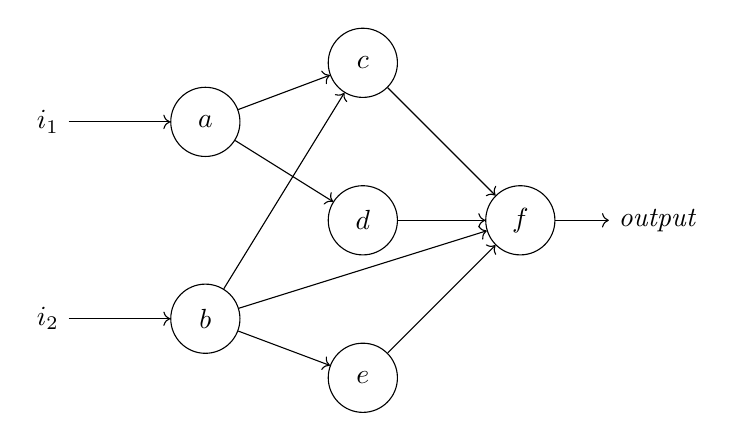
\begin{tikzpicture}
\node (i1)[] at (0, 3.25) {$i_1$};
\node (i2)[] at (0, 0.75) {$i_2$};
\node (a)[circle, draw, minimum width=25pt] at (2, 3.25) {$a$};
\node (b)[circle, draw, minimum width=25pt] at (2, 0.75) {$b$};
\node (c)[circle, draw, minimum width=25pt] at (4, 4) {$c$};
\node (d)[circle, draw, minimum width=25pt] at (4, 2) {$d$};
\node (e)[circle, draw, minimum width=25pt] at (4, 0) {$e$};
\node (f)[circle, draw, minimum width=25pt] at (6, 2) {$f$};
\node (output)[] at (7.75, 2) {$\mathit{output}$};
\draw[->] (i1) -- (a) ;
\draw[->] (i2) -- (b) ;
\draw[->] (a) -- (c);
\draw[->] (a) -- (d);
% \draw[->] (a) -- (e);
\draw[->] (b) -- (c);
\draw[->] (b) -- (f);
\draw[->] (b) -- (e);
\draw[->] (c) -- (f);
\draw[->] (d) -- (f);
\draw[->] (e) -- (f);
\draw[->] (f) -- (output);
\end{tikzpicture}
\end{minipage}~\\[2.5pt]
\scalebox{0.7}{
\begin{tikzpicture}
\node[draw,minimum width=0.5cm, minimum height=0.5cm] at (0,0) {0};
\node[draw,minimum width=0.5cm, minimum height=0.5cm] at (0.5,0) {0};
\node[draw,minimum width=0.5cm, minimum height=0.5cm] at (1,0) {0};
\node[draw,minimum width=0.5cm, minimum height=0.5cm] at (1.5,0) {0};
\node[draw,minimum width=0.5cm, minimum height=0.5cm] at (2,0) {0};
\node[draw,minimum width=0.5cm, minimum height=0.5cm] at (2.5,0) {0};
\node[draw,minimum width=0.5cm, minimum height=0.5cm] at (3,0) {0};
\node[draw,minimum width=0.5cm, minimum height=0.5cm] at (3.5,0) {0};
\node[draw,minimum width=0.5cm, minimum height=0.5cm] at (4,0) {0};
\node[draw,minimum width=0.5cm, minimum height=0.5cm] at (4.5,0) {0};
\node[draw,minimum width=0.5cm, minimum height=0.5cm] at (5,0) {0};
\node[draw,minimum width=0.5cm, minimum height=0.5cm] at (5.5,0) {0};
\node[draw,minimum width=0.5cm, minimum height=0.5cm,fill=hured!20] at (6,0) {1};
\node[draw,minimum width=0.5cm, minimum height=0.5cm,fill=hured!20] at (6.5,0) {1};
\node[draw,minimum width=0.5cm, minimum height=0.5cm] at (7,0) {0};
\node[draw,minimum width=0.5cm, minimum height=0.5cm] at (7.5,0) {0};
\node[draw,minimum width=0.5cm, minimum height=0.5cm] at (8,0) {0};
\node[draw,minimum width=0.5cm, minimum height=0.5cm] at (8.5,0) {0};
\node[draw,minimum width=0.5cm, minimum height=0.5cm,fill=hured!20] at (9,0) {1};
\node[draw,minimum width=0.5cm, minimum height=0.5cm] at (9.5,0) {0};
\node[draw,minimum width=0.5cm, minimum height=0.5cm] at (10,0) {0};
\node[draw,minimum width=0.5cm, minimum height=0.5cm] at (10.5,0) {0};
\node[draw,minimum width=0.5cm, minimum height=0.5cm] at (11,0) {0};
\node[draw,minimum width=0.5cm, minimum height=0.5cm] at (11.5,0) {0};
\node[draw,minimum width=0.5cm, minimum height=0.5cm] at (12,0) {0};
\node[draw,minimum width=0.5cm, minimum height=0.5cm,fill=hured!20] at (12.5,0) {1};
\node[draw,minimum width=0.5cm, minimum height=0.5cm] at (13,0) {0};
\node[draw,minimum width=0.5cm, minimum height=0.5cm] at (13.5,0) {0};
\node[draw,minimum width=0.5cm, minimum height=0.5cm] at (14,0) {0};
\node[draw,minimum width=0.5cm, minimum height=0.5cm] at (14.5,0) {0};
\node[draw,minimum width=0.5cm, minimum height=0.5cm] at (15,0) {0};
\node[draw,minimum width=0.5cm, minimum height=0.5cm,fill=hured!20] at (15.5,0) {1};
\node[draw,minimum width=0.5cm, minimum height=0.5cm,fill=hured!20] at (16,0) {1};
\node[draw,minimum width=0.5cm, minimum height=0.5cm,fill=hured!20] at (16.5,0) {1};
\node[draw,minimum width=0.5cm, minimum height=0.5cm,fill=hured!20] at (17,0) {1};
\node[draw,minimum width=0.5cm, minimum height=0.5cm] at (17.5,0) {0};
\node at (1,1) {Chromosome:};
\draw[ultra thick] (-0.25,-0.25) rectangle (2.75,0.25);
\draw[ultra thick] (2.75,-0.25) rectangle (5.75,0.25);
\draw[ultra thick] (5.75,-0.25) rectangle (8.75,0.25);
\draw[ultra thick] (8.75,-0.25) rectangle (11.75,0.25);
\draw[ultra thick] (11.75,-0.25) rectangle (14.75,0.25);
\draw[ultra thick] (14.75,-0.25) rectangle (17.75,0.25);
\draw[decorate,decoration={brace,amplitude=10pt}] (2.75,-0.5) -- (-0.25, -0.5);
\node at (1.25, -1) {Gene};
\end{tikzpicture}}
\end{center}
We now apply our typical evolutionary components (fitness, selection, recombination, etc.) to obtain the following optimisation cycle:
\begin{center}
\newcommand\neuralnet[4]{
  \foreach \x in {0,...,36} {
    \draw (#1+\x*0.1, #2) rectangle (#1+0.1+\x*0.1,#2+0.25);
  }
  \foreach \x in {#3} {
    \draw[fill=hured!60] (#1+\x*0.1, #2) rectangle (#1+0.1+\x*0.1, #2+0.25);
  }
}
\begin{tikzpicture}
% \draw[step=1cm, gray, thin] (0,0) grid (12, 12);
% Current Generation genomes
\draw[fill=white] (4,12) rectangle (8,8);
\draw[fill=white] (4.1,11.9) rectangle (8.1,7.9);
\draw[fill=white] (4.2,11.8) rectangle (8.2,7.8);
% Top individual title
\node at (6.2, 11.5) {\textit{neural network}}; 
% Top individual genome
\neuralnet{4.35}{10.5}{12,13,18,25,26,32,33,34,35};
% Top individual neural net
\node (i1)[] at (4.55, 9.75) {\tiny $i_1$};
\node (i2)[] at (4.55, 9) {\tiny $i_2$};
\node (a)[circle, draw] at (5.35, 9.75) {\tiny $a$};
\node (b)[circle, draw] at (5.35, 9) {\tiny $b$};
\node (c)[circle, draw] at (6.5, 10) {\tiny $c$};
\node (d)[circle, draw] at (6.5, 9.25) {\tiny $d$};
\node (e)[circle, draw] at (6.5, 8.5) {\tiny $e$};
\node (f)[circle, draw] at (7.35, 9) {\tiny $f$};
\node (output)[] at (8.1, 9) {};
\draw[->] (i1) -- (a) ;
\draw[->] (i2) -- (b) ;
\draw[->] (a) -- (c);
\draw[->] (a) -- (d);
% \draw[->] (a) -- (e);
\draw[->] (b) -- (c);
\draw[->] (b) -- (f);
\draw[->] (b) -- (e);
\draw[->] (c) -- (f);
\draw[->] (d) -- (f);
\draw[->] (e) -- (f);
\draw[->] (f) -- (output);
\node at (6.2, 8.1) {\footnotesize\textit{fitness}$=117$};

\draw[fill=white] (-1,4) rectangle (3,8);
\node at (1, 7.75) {\textit{generation} $i$};
\neuralnet{-0.85}{7.25}{12,13,18,25,26,32,33,34,35};
\neuralnet{-0.85}{6.75}{12,18,24,25,30,31,32,33,34,35};
\neuralnet{-0.85}{6.25}{12,13,19,24,30,32,33,34};
\neuralnet{-0.85}{5.75}{12,18,25,32,35};
\neuralnet{-0.85}{5.25}{13,18,19,24,25,33,34,35};
\neuralnet{-0.85}{4.75}{12,19,24,30,31,34,35};
\neuralnet{-0.85}{4.25}{12,13,18,25,31,32,33,34,35};
\draw[fill=white] (0, 4.25) rectangle (4, 0.25);
\node at (2, 4) {\textit{generation} $i+1$};
\neuralnet{0.15}{3.5}{12,13,18,25,26,32,33,34,35};
\neuralnet{0.15}{3}{12,13,18,24,30,32,33,34,35};
\neuralnet{0.15}{2.5}{12,13,19,25,32,33,34};
\neuralnet{0.15}{2}{12,13,18,24,30,32,34,35};
\neuralnet{0.15}{1.5}{12,18,25,32,35};
\neuralnet{0.15}{1}{13,18,19,24,25,33,34,35};
\neuralnet{0.15}{0.5}{12,13,18,25,31,32,33,34,35};

\draw[fill=white] (9, 8) rectangle (13, 4.5);
\node at (11, 7.75) {\textit{crossover}};
\neuralnet{9.15}{7}{12,13,18,25,26,32,33,34,35};
\neuralnet{9.15}{6.25}{12,13,19,24,30,32,33,34};
\draw[fill=white,white] (11.55, 7.30) rectangle (12.25, 6.2);
  \draw[fill=white] (11.6, 7.1) rectangle (11.7, 7.35);
  \draw[fill=hured!60] (11.7, 7.1) rectangle (11.8, 7.35);
  \draw[fill=hured!60] (11.8, 7.1) rectangle (11.9, 7.35);
  \draw[fill=white] (11.9, 7.1) rectangle (12.0, 7.35);
  \draw[fill=white] (12.0, 7.1) rectangle (12.1, 7.35);
  \draw[fill=white] (12.1, 7.1) rectangle (12.2, 7.35);
  \draw[fill=white] (12.2, 7.1) rectangle (12.3, 7.35);
  \draw[fill=hured!60] (11.6, 6.35) rectangle (11.7, 6.6);
  \draw[fill=white] (11.7, 6.35) rectangle (11.8, 6.6);
  \draw[fill=white] (11.8, 6.35) rectangle (11.9, 6.6);
  \draw[fill=white] (11.9, 6.35) rectangle (12.0, 6.6);
  \draw[fill=white] (12.0, 6.35) rectangle (12.1, 6.6);
  \draw[fill=white] (12.1, 6.35) rectangle (12.2, 6.6);
  \draw[fill=hured!60] (12.2, 6.35) rectangle (12.3, 6.6);
  \draw[<->] (12, 7.05) to (12, 6.65);
\node[anchor=west] at (9.15, 5.85) {\textit{children:}};
\neuralnet{9.15}{5.25}{12,13,18,24,30,32,33,34,35};
\neuralnet{9.15}{4.75}{12,13,19,25,26,32,33,34};
\draw[fill=white] (9, 3) rectangle (13, 1);
\node at (11, 2.75) {\textit{mutation}};
\neuralnet{9.15}{2}{12,13,18,24,30,32,33,34,35};
\node at (12.5,2.1) {x};
\draw[->] (12.5, 1.9) to (12.5, 1.6);
\neuralnet{9.15}{1.25}{12,13,18,24,30,32,34,35};

\draw[fill=white] (4.5, 6.5) rectangle (8, 2.25);
\node at (6.25, 6.25) {\textit{training data set}};
\node at (6.25,4.1) {\scriptsize
$\begin{array}{rrr}
0&0&1.0000\\
0.1000&0.0998&0.8869\\
0.2000&0.1987&0.7551\\
0.3000&0.2955&0.6142\\
0.4000&0.3894&0.4720\\
0.5000&0.4794&0.3345\\
0.6000&0.5646&0.2060\\
0.7000&0.6442&0.0892\\
0.8000&0.7174&-0.0143\\
0.9000&0.7833&-0.1038\\
1.0000& 0.8415&-0.1794
\end{array}$
};

% Arrows $
\draw[blArrow] (11, 4.4) to (11, 3.1);
\draw[blArrow] (11, 0.9) -- (11, -0.75) -- (1.5, -0.75) to (1.5, 0.15);
\draw[blArrow] (1.5, 8.1) -- (1.5, 10) to (3.9, 10);
\draw[blArrow] (8.3, 10) -- (11, 10) to (11, 8.1);
\draw[blArrow] (6.25, 6.6) to (6.25, 7.7);
\node at (10, 10.5) {\textit{selection}};
\end{tikzpicture}
\end{center}

This method of encoding (called \textit{direct encoding}) and evolving the topology of neural networks becomes increasingly cumbersome when the complexity of the network rises (when more and more nodes are added). As the size of the network grows, the size of the required chromosome increases quickly, leading to problems in performance. Moreover, direct encoding cannot represent repeated or nested structures in the network, which are common for some problems.

An alternative encoding, called \textit{grammatical encoding} tries to solve this problem. This encoding represents the network encoding as grammars; the genetic algorithm evolves the grammars, but the fitness is tested only after a ``development'' step in which a network develops from the grammar. That is, the grammar is a ``genotype'', while the ``phenotype'' is a network derived from that grammar. The exact encoding scheme used in this method, and the execution of it are beyond the scope of this discussion.


\subsection{Evolving weights}
While this subject is beyond the scope of this course, as we have learned back-propagation in Section \ref{sec:gradient}. Back-propagation is in most situation the better way of learning the weights in a neural network, and is therefore preferred. In some situations, however, back-propagation can get stuck in one of the many local optima present, and has difficulties escaping these. In such cases, using a genetic algorithm to learn the weights instead could be helpful.

To apply genetic algorithms to the learning of weights, we use the vector representation as presented in the previous chapter. The chromosomes in our population are a sequence of (real) numbers, where each number represents a weight of a connection in the neural network. We group numbers related to a single neuron in a gene:
\begin{center}
\begin{tikzpicture}
\node (a)[circle, draw, minimum width=25pt] at (2, 1) {$a$};
\node (b)[circle, draw, minimum width=25pt] at (2, 0) {$b$};
\node (c)[circle, draw, minimum width=25pt] at (2, -1) {$c$};
\node (d)[circle, draw, minimum width=25pt] at (4, 1.5) {$d$};
\node (e)[circle, draw, minimum width=25pt] at (4, 0.5) {$e$};
\node (f)[circle, draw, minimum width=25pt] at (4, -0.5) {$f$};
\node (g)[circle, draw, minimum width=25pt] at (4, -1.5) {$g$};
\node (h)[circle, draw, minimum width=25pt] at (6, 0) {$h$};
\node (i1)[] at (0, 1) {$i_1$};
\node (i2)[] at (0, 0) {$i_2$};
\node (i3)[] at (0, -1) {$i_3$};
\node (output)[] at (7.75, 0) {$\mathit{output}$};
\draw[->] (i1) -- (a) ;
\draw[->] (i2) -- (b) ;
\draw[->] (i3) -- (c) ;
\draw[->,hured] (a) -- (d);
\draw[->] (a) -- (e);
\draw[->] (a) -- (f);
\draw[->] (a) -- (g);
\draw[->,hured] (b) -- (d);
\draw[->] (b) -- (e);
\draw[->] (b) -- (f);
\draw[->] (b) -- (g);
\draw[->,hured] (c) -- (d);
\draw[->] (c) -- (e);
\draw[->] (c) -- (f);
\draw[->] (c) -- (g);
\draw[->,hublue] (d) -- (h);
\draw[->,hublue] (e) -- (h);
\draw[->,hublue] (f) -- (h);
\draw[->,hublue] (g) -- (h);
\draw[->] (h) -- (output);

\node[anchor=south west] at (-2,-2.5) {Chromosome:};
\node[anchor=south west,draw,minimum height=1cm,minimum width=1cm,fill=hured!20] at (-2,-3.5) {\footnotesize $w_{a\rightarrow d}$};
\node[anchor=south west,draw,minimum height=1cm,minimum width=1cm,fill=hured!20] at (-1,-3.5) {\footnotesize $w_{b\rightarrow d}$};
\node[anchor=south west,draw,minimum height=1cm,minimum width=1cm,fill=hured!20] at (0,-3.5) {\footnotesize $w_{c\rightarrow d}$};
\node[anchor=south west,draw,minimum height=1cm,minimum width=1cm] at (1,-3.5) {\footnotesize $w_{a\rightarrow e}$};
\node[anchor=south west,draw,minimum height=1cm,minimum width=1cm] at (2,-3.5) {\footnotesize $w_{b\rightarrow e}$};
\node[anchor=south west,draw,minimum height=1cm,minimum width=1cm] at (3,-3.5) {\footnotesize $w_{c\rightarrow e}$};
\node[anchor=south west] at (4.15,-3.25) {\ldots};
\node[anchor=south west,draw,minimum height=1cm,minimum width=1cm] at (5,-3.5) {\footnotesize $w_{c\rightarrow g}$};
\node[anchor=south west,draw,minimum height=1cm,minimum width=1cm,fill=hublue!20] at (6,-3.5) {\footnotesize $w_{d\rightarrow h}$};
\node[anchor=south west,draw,minimum height=1cm,minimum width=1cm,fill=hublue!20] at (7,-3.5) {\footnotesize $w_{e\rightarrow h}$};
\node[anchor=south west,draw,minimum height=1cm,minimum width=1cm,fill=hublue!20] at (8,-3.5) {\footnotesize $w_{f\rightarrow h}$};
\node[anchor=south west,draw,minimum height=1cm,minimum width=1cm,fill=hublue!20] at (9,-3.5) {\footnotesize $w_{g\rightarrow h}$};
\draw[decorate,decoration={brace,amplitude=10pt}] (1, -3.75) -- (-2, -3.75);
\node at (-0.5, -4.5) {Gene};
\end{tikzpicture}
\end{center}

Next we need to define a fitness function for evaluating the performance of the chromosomes. The function must estimate the performance of a given network, which can easily be calculated by having the network classify a number of examples. The number of examples should not be too small, since this increases the risk of overfitting (the neural network performs well on the examples, but not on the real problem). However, too much examples means that the evaluation of a population takes more time. An alternative is to select a portion of a large data set for testing every selection round (but make sure that all networks are scored using the same examples).

The simplest function to score networks (based on an example set) is using the sum of squared errors (see Section \ref{sec:gradient} earlier for details). The smaller the sum, the fitter the network. This means that the genetic algorithm attempts to find a set of weights that minimises the sum of squared errors.

There are a number of choices for the genetic operators. In some cases, an evolutionary strategy is used which means that only mutation is allowed, but crossover can be applied as well, if designed correctly. A crossover operator (single-point crossover, two-point crossover, or even uniform crossover) needs to adhere to the weights that belong to a single neuron; that is, crossover can be performed, as long as the crossover points are chosen to match the gene encoding, that is, split only on the segments that represent the weights on the links related to a single neuron.
\begin{center}
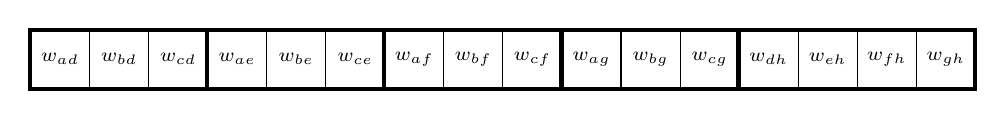
\begin{tikzpicture}[font=\scriptsize]
\node[anchor=south west,thin,draw,minimum width=0.75cm,minimum height=0.75cm] at (0,   0) {$w_{ad}$};
\node[anchor=south west,thin,draw,minimum width=0.75cm,minimum height=0.75cm] at (0.75,0) {$w_{bd}$};
\node[anchor=south west,thin,draw,minimum width=0.75cm,minimum height=0.75cm] at (1.5, 0) {$w_{cd}$};
\node[anchor=south west,thin,draw,minimum width=0.75cm,minimum height=0.75cm] at (2.25,0) {$w_{ae}$};
\node[anchor=south west,thin,draw,minimum width=0.75cm,minimum height=0.75cm] at (3,   0) {$w_{be}$};
\node[anchor=south west,thin,draw,minimum width=0.75cm,minimum height=0.75cm] at (3.75,0) {$w_{ce}$};
\node[anchor=south west,thin,draw,minimum width=0.75cm,minimum height=0.75cm] at (4.5, 0) {$w_{af}$};
\node[anchor=south west,thin,draw,minimum width=0.75cm,minimum height=0.75cm] at (5.25,0) {$w_{bf}$};
\node[anchor=south west,thin,draw,minimum width=0.75cm,minimum height=0.75cm] at (6,   0) {$w_{cf}$};
\node[anchor=south west,thin,draw,minimum width=0.75cm,minimum height=0.75cm] at (6.75,0) {$w_{ag}$};
\node[anchor=south west,thin,draw,minimum width=0.75cm,minimum height=0.75cm] at (7.5, 0) {$w_{bg}$};
\node[anchor=south west,thin,draw,minimum width=0.75cm,minimum height=0.75cm] at (8.25,0) {$w_{cg}$};
\node[anchor=south west,thin,draw,minimum width=0.75cm,minimum height=0.75cm] at (9,   0) {$w_{dh}$};
\node[anchor=south west,thin,draw,minimum width=0.75cm,minimum height=0.75cm] at (9.75,0) {$w_{eh}$};
\node[anchor=south west,thin,draw,minimum width=0.75cm,minimum height=0.75cm] at (10.5,0) {$w_{fh}$};
\node[anchor=south west,thin,draw,minimum width=0.75cm,minimum height=0.75cm] at (11.25,0) {$w_{gh}$};
\draw[ultra thick] (0,0) rectangle (2.25,0.75);
\draw[ultra thick] (2.25,0) rectangle (4.5,0.75);
\draw[ultra thick] (4.5,0) rectangle (6.75,0.75);
\draw[ultra thick] (6.75,0) rectangle (9,0.75);
\draw[ultra thick] (9,0) rectangle (12, 0.75);
% \draw[ultra thick] (2.25, 1.25) -- (2.25, -0.5)
%                    (4.5,  1.25) -- (4.5,  -0.5)
%                    (6.75, 1.25) -- (6.75, -0.5)
%                    (9,    1.25) -- (9,    -0.5);
\end{tikzpicture}
\end{center}

The mutation operator can be chosen, for instance, to add a small random value between $-1$ and $1$ to each weight in a randomly chosen gene (again, remember that a single gene represents multiple weights).

As mentioned at the start of this section, while the optimisation of weights of a neural network by means of an evolutionary algorithm is possible, it is rarely used. This is because the genetic algorithm has many more parameters that need to be selected to find the optimal training strategy, and because back-propagation usually functions well enough. The latter is especially true in larger (thousands to millions of neurons) networks.

\section{Exercises}
%Choose and solve either exercise \ref{ex:card} or \ref{ex:wing}; they are different flavours of the same kind of problem:
\begin{exercise}[Card problem]\label{ex:card}~\\
You have 10 cards numbered from 1 to 10. You have to choose a way of dividing them into two piles, so that the cards in the first pile \textbf{sum} to a number as close as possible to 36, and the remaining cards in the other pile \textbf{multiply} to a number as close as possible to 360.

\paragraph{Genotype encoding}
Each card can be put in \pythoninline{Pile_0} or \pythoninline{Pile_1}, there are 1024 possible ways of sorting them into two piles, and you have to find the best. Think of a sensible way of encoding any possible solution-attempt as a genotype.

\paragraph{Fitness}
Some of these solution attempts will be closer to the target than others. Think of a sensible way of evaluating any solution-attempt and scoring it with a fitness-measure.

\paragraph{Assignment}
Write a program to run a Genetic Algorithm with your genotype encoding and fitness function.
Run it once for a suitable (probably very large -- you choose) number of generations.
Then repeat that same run a number of times (like, 100) and see if you get the same answer each time, see how much variance there is between each run.
\end{exercise}

\begin{exercise}[Wing design]\label{ex:wing}~\\
You have 4 variables that represent possible parameter settings for the design of an aircraft wing. $A$, $B$, $C$, and $D$, each of which can be any whole number between 0 and 63 (use a bit encoding per parameter).

\noindent Your aerodynamics model tells you that the $\mathit{Lift}$ of the wing is the following:
$$\mathit{Lift} = (A-B)^2+(C+D)^2-(A-30)^3-(C-40)^3$$

\noindent Find values of $A$ $B$ $C$ $D$, each within their allowed range 0-63, that maximises $\mathit{Lift}$.

\paragraph{Assignment}
Write a program to run a Genetic Algorithm with your genotype encoding and fitness function.
Run it once for a suitable (probably very large -- you choose) number of generations.
Then repeat that same run a number of times (like, 100) and see if you get the same answer each time, see how much variance there is between each run.
\end{exercise}

\begin{exercise}[Face Recognition (Optional)]~\\
In this exercise we are going to combine evolutionary algorithms with neural networks to create a facial recognition system.

A data set consisting of pictures (96$\times$96 pixels, greyscale) is available on the electronic learning environment. The images are pictures (centered) of lecturers of the Computer Engineering team. Your task is to use the available data set to create and train a neural network that can detect which person is represented on a given image.

Use an evolutionary algorithm to determine the most suitable configuration (topology, etc.) of your neural network. The neural networks should be created by using available library implementation\footnote{For example, see Appendix \ref{ch:lib} for descriptions of the use of neural network libraries, including \pythoninline{TensorFlow} and \pythoninline{Theano}. You are not restricted to either of these, you may choose your own.}

The optimisation of the network and the training of the neural network are done in \textit{your} time; during grading we will assess how well your (best) neural network performs on a new set of images. That means that you need to be able to save (and later load) a neural network (layers, weights, etc.).

\paragraph{Hand-in}
You need to hand-in the following elements:
\begin{itemize}
\item the implementation (code) of the evolutionary algorithm that was used to determine the NN architecture;
\item a short description of the best architecture (found by your EA) (describe number of layers, layer types, etc.) and a brief explanation why you think this is the best architecture;
\item an implementation (code) that can read your best network and perform a classification based on a given (similar, but different) dataset to assess it's performance.
\end{itemize}
\end{exercise}


\part{Uitwerkingen}
\section{Neural Networks}

\begin{enumerate}[label=2.\arabic*, itemsep=8pt]
	\item Logische poorten
	\begin{enumerate}[itemsep=8pt]
		\item De inputs/output geven de waarheidstabel van een AND-poort:
		\begin{itemize}
			\item $x_1 = 0$; $x_2 = 0$ geeft $0 \times 0.5 + 0 \times 0.5 - 1.0 = -1.0 < 0$ dus $g = 0$
			\item $x_1 = 0$; $x_2 = 1$ geeft $0 \times 0.5 + 1 \times 0.5 - 1.0 = -0.5 < 0$ dus $g = 0$
			\item $x_1 = 1$; $x_2 = 0$ geeft $1 \times 0.5 + 0 \times 0.5 - 1.0 = -0.5 < 0$ dus $g = 0$
			\item $x_1 = 1$; $x_2 = 1$ geeft $1 \times 0.5 + 1 \times 0.5 - 1.0 = 0.0 = 0$ dus $g = 1$
		\end{itemize}

		\item De inputs/output geven de waarheidstabel van een OR-poort:
		\begin{itemize}
			\item $x_1 = 0$; $x_2 = 0$ geeft $0 \times 0.5 + 0 \times 0.5 - 0.5 = -0.5 < 0$ dus $g = 0$
			\item $x_1 = 0$; $x_2 = 1$ geeft $0 \times 0.5 + 1 \times 0.5 - 0.5 = 0.0 = 0$ dus $g = 1$
			\item $x_1 = 1$; $x_2 = 0$ geeft $1 \times 0.5 + 0 \times 0.5 - 0.5 = 0.0 = 0$ dus $g = 1$
			\item $x_1 = 1$; $x_2 = 1$ geeft $1 \times 0.5 + 1 \times 0.5 - 0.5 = 0.5 > 0$ dus $g = 1$
		\end{itemize}

		\item De input/output geeft de waarheidstabel van een INVERT-poort (met andere woorden, de logische NOT):
		\begin{itemize}
			\item $x_1 = 0$ geeft $0 \times -1 + 0.5 = 0.5 > 0$ dus $g = 1$
			\item $x_1 = 1$ geeft $1 \times -1 + 0.5 = -0.5 < 0$ dus $g = 0$
		\end{itemize}	
	\end{enumerate}


	\item PARTY-poort
	\begin{enumerate}[itemsep=8pt]
		\item Bijvoorbeeld: $x_1 = x_2 = x_3 = 1$ geeft \\ $1 \times 0.6 + 1 \times 0.3 + 1 \times 0.2 - 0.4 = 0.7 > 0$ dus $g = 1$

		\begin{tabular}{c|c|c|c|c}
		      $x_1$ 			& $x_2$ 			& $x_3$			& gewogen som			& $g$	\\
		      \hline
		      0				& 0				& 0 				& $-0.4 < 0$			& 0		\\
		      0				& 0				& 1 				& $-0.2 < 0$			& 0		\\
		      0				& 1				& 0 				& $-0.1 < 0$			& 0		\\
		      0				& 1				& 1 				& $0.1 > 0$			& 1		\\
		      1				& 0				& 0 				& $0.2 > 0$			& 1		\\
		      1				& 0				& 1 				& $0.4 > 0$			& 1		\\
		      1				& 1				& 0 				& $0.5 > 0$			& 1		\\
		      1				& 1				& 1 				& $0.7 > 0$			& 1		\\
	    \end{tabular}

	    	\item Bijvoorbeeld: $x_1 = x_2 = x_3 = 1$ geeft \\ $1 \times 0.1 + 1 \times 0.3 + 1 \times 0.2 - 0.9 = -0.3 < 0$ dus $g = 0$

		\begin{tabular}{c|c|c|c|c}
		      $x_1$ 			& $x_2$ 			& $x_3$			& gewogen som			& $g$	\\
		      \hline
		      0				& 0				& 0 				& $-0.9 < 0$			& 0		\\
		      0				& 0				& 1 				& $-0.7 < 0$			& 0		\\
		      0				& 1				& 0 				& $-0.6 < 0$			& 0		\\
		      0				& 1				& 1 				& $-0.4 < 0$			& 0		\\
		      1				& 0				& 0 				& $-0.8 < 0$			& 0		\\
		      1				& 0				& 1 				& $-0.6 < 0$			& 0		\\
		      1				& 1				& 0 				& $-0.5 < 0$			& 0		\\
		      1				& 1				& 1 				& $-0.3 < 0$			& 0		\\
	    \end{tabular}
    	\end{enumerate}


	\item NOR-poort: zie figuur \ref{fig:nor_gate}.
		\begin{figure}[h!]
		\centering
		\begin{tikzpicture}[scale=1, transform shape]
			\node (a)[circle, draw] at (4, 0) {$b = 0.0$};
			\node (x1)[] at (0, 2) {$x_1$};
			\node (x2)[] at (0, 0) {$x_2$};
			\node (x3)[] at (0, -2) {$x_3$};
			\node (output)[] at (7, 0) {output};
			\draw[->] (x1) -- (a) node[pos=0.3,sloped,above] {\small $w_1 = -1$};
			\draw[->] (x2) -- (a) node[pos=0.35,sloped,above] {\small $w_2 = -1$};
			\draw[->] (x3) -- (a) node[pos=0.4,sloped,above] {\small $w_3 = -1$};
			\draw[->] (a) -- (output);
		\end{tikzpicture}
		\caption{Oplossing NOR-poort}
		\label{fig:nor_gate}
		\end{figure}



	\item XOR-poort: zie figuur \ref{fig:xor_gate}.
		\begin{figure}
		\centering
		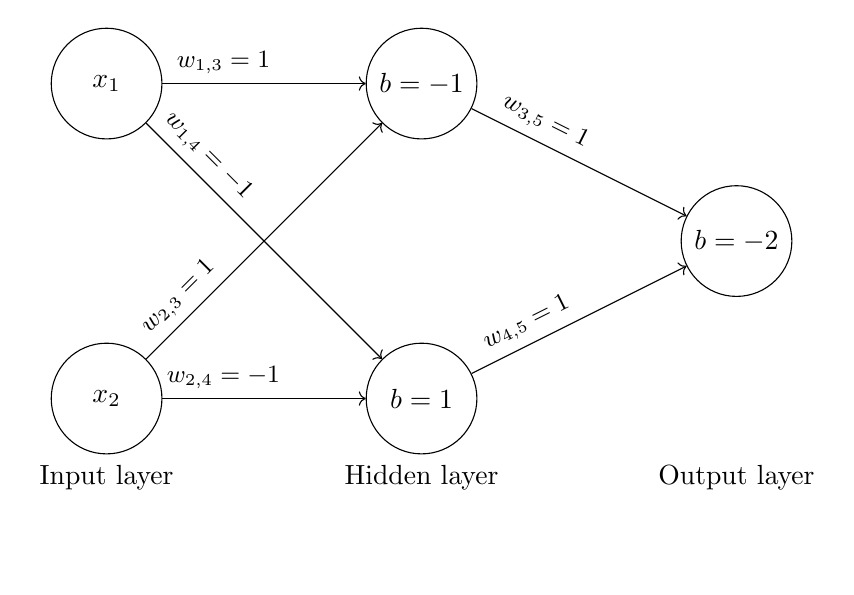
\begin{tikzpicture}[scale=1, transform shape]
			\node (x1)[circle, draw, minimum width=40pt] at (0, 2) {$x_1$};
			\node (x2)[circle, draw, minimum width=40pt] at (0, -2) {$x_2$};
			\node (IL)[circle] at (0, -3) {Input layer};

			\node (a)[circle, draw, minimum width=40pt] at (4, 2) {$b = -1$};
			\node (b)[circle, draw, minimum width=40pt] at (4, -2) {$b = 1$};
			\node (HL)[circle] at (4, -3) {Hidden layer};

			\node (c)[circle, draw, minimum width=40pt] at (8, 0) {$b = -2$};
			\node (OL)[circle] at (8, -3) {Output layer};

			\draw[->] (x1) -- (a) node[pos=0.3,sloped,above] {\small $w_{1,3} =  1$};
			\draw[->] (x1) -- (b) node[pos=0.2,sloped,above] {\small $w_{1,4} = -1$};
			\draw[->] (x2) -- (a) node[pos=0.2,sloped,above] {\small $w_{2,3} =  1$};
			\draw[->] (x2) -- (b) node[pos=0.3,sloped,above] {\small $w_{2,4} = -1$};

			\draw[->] (a) -- (c) node[pos=0.3,sloped,above] {\small $w_{3,5} = 1$};
			\draw[->] (b) -- (c) node[pos=0.3,sloped,above] {\small $w_{4,5} = 1$};
		\end{tikzpicture}
		\caption{Oplossing XOR-poort: de bovenste node van de hidden layer is een OR-poort en de onderste is een NAND-poort; de outputnode is een AND-poort.}
		\label{fig:xor_gate}
		\end{figure}


	\item Half adder: zie figuur \ref{fig:adder}.
		\begin{figure}
		\centering
		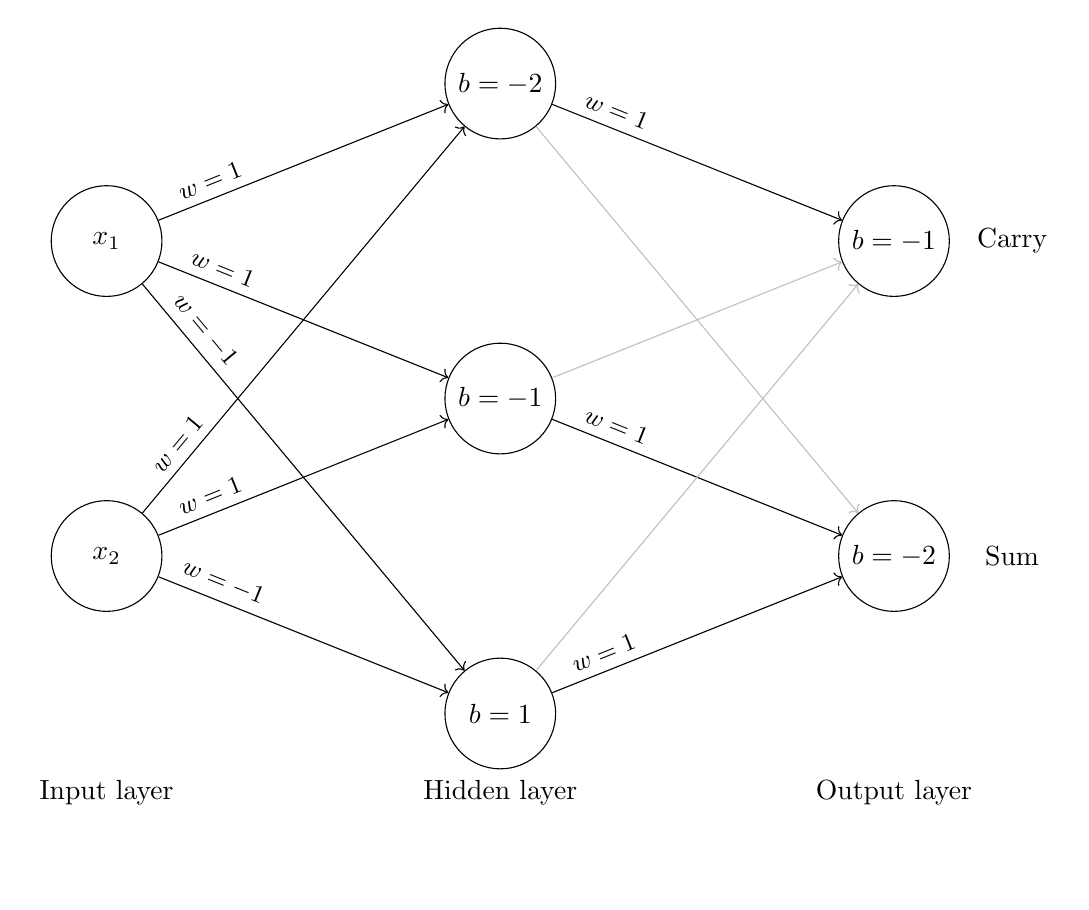
\begin{tikzpicture}[scale=1, transform shape]
			\node (x1)[circle, draw, minimum width=40pt] at (0, 2) {$x_1$};
			\node (x2)[circle, draw, minimum width=40pt] at (0, -2) {$x_2$};
			\node (IL)[circle] at (0, -5) {Input layer};

			\node (f)[circle, draw, minimum width=40pt] at (5, 4) {$b = -2$};
			\node (g)[circle, draw, minimum width=40pt] at (5, 0) {$b = -1$};
			\node (h)[circle, draw, minimum width=40pt] at (5, -4) {$b = 1$};
			\node (HL)[circle] at (5, -5) {Hidden layer};

			\node (c)[circle, draw, minimum width=40pt] at (10, 2) {$b = -1$};
			\node (CL)[circle] at (11.5, 2) {Carry};
			\node (s)[circle, draw, minimum width=40pt] at (10, -2) {$b = -2$};
			\node (SL)[circle] at (11.5, -2) {Sum};
			\node (OL)[circle] at (10, -5) {Output layer};


			\draw[->] (x1) -- (f) node[pos=0.2,sloped,above] {\small $w = 1$};
			\draw[->] (x1) -- (g) node[pos=0.2,sloped,above] {\small $w = 1$};
			\draw[->] (x1) -- (h) node[pos=0.15,sloped,above] {\small $w = -1$};
			\draw[->] (x2) -- (f) node[pos=0.15,sloped,above] {\small $w = 1$};
			\draw[->] (x2) -- (g) node[pos=0.2,sloped,above] {\small $w = 1$};
			\draw[->] (x2) -- (h) node[pos=0.2,sloped,above] {\small $w = -1$};

			\draw[->] (f) -- (c) node[pos=0.2,sloped,above] {\small $w =  1$};
			\draw[->, lightgray] (f) -- (s) node[pos=0.2,sloped,above] {};
			\draw[->, lightgray] (g) -- (c) node[pos=0.2,sloped,above] {};
			\draw[->] (g) -- (s) node[pos=0.2,sloped,above] {\small $w =  1$};
			\draw[->, lightgray] (h) -- (c) node[pos=0.2,sloped,above] {};
			\draw[->] (h) -- (s) node[pos=0.2,sloped,above] {\small $w = 1$};
		\end{tikzpicture}
		\caption{Oplossing half-adder. De sum is een XOR en de carry is een AND. De bovenste outputnode is de carry en de onderste is de sum. De bovenste hidden node is de AND en de carry zelf doet niets. De onderste twee hidden nodes en de sumnode zijn samen een XOR (zie boven). De grijze verbindingen hebben $w=0$.}
		\label{fig:adder}
		\end{figure}


	\item Bitwise representation: zie figuur \ref{fig:bitwise}.
		\begin{figure}
		\centering
		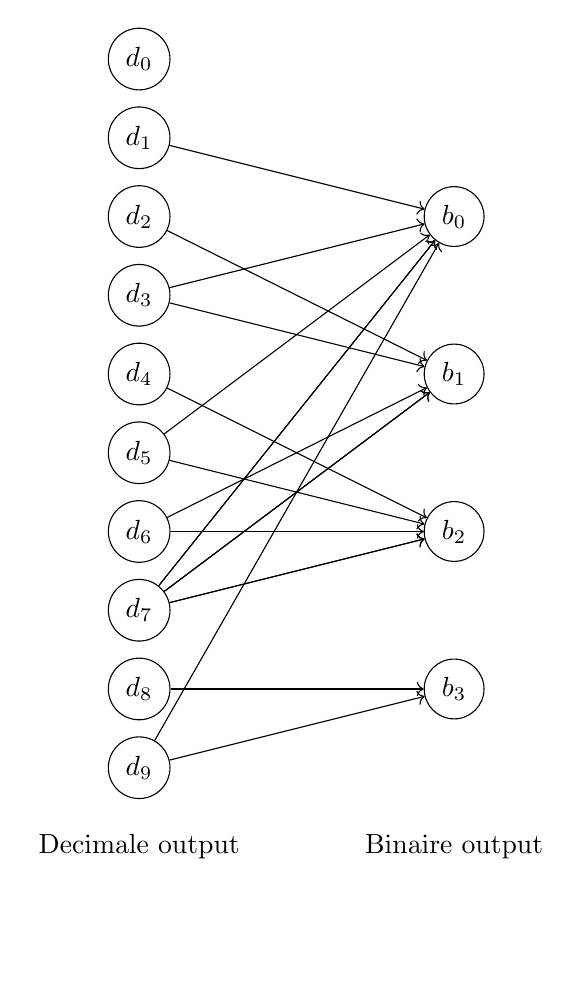
\begin{tikzpicture}[scale=1, transform shape]
			\node (x0)[circle, draw] at (0,  0) {$d_0$};
			\node (x1)[circle, draw] at (0, -1) {$d_1$};
			\node (x2)[circle, draw] at (0, -2) {$d_2$};
			\node (x3)[circle, draw] at (0, -3) {$d_3$};
			\node (x4)[circle, draw] at (0, -4) {$d_4$};
			\node (x5)[circle, draw] at (0, -5) {$d_5$};
			\node (x6)[circle, draw] at (0, -6) {$d_6$};
			\node (x7)[circle, draw] at (0, -7) {$d_7$};
			\node (x8)[circle, draw] at (0, -8) {$d_8$};
			\node (x9)[circle, draw] at (0, -9) {$d_9$};
			\node (IL)[circle] at (0, -10) {Decimale output};

			\node (b1)[circle, draw] at (4, -2) {$b_0$};
			\node (b2)[circle, draw] at (4, -4) {$b_1$};
			\node (b3)[circle, draw] at (4, -6) {$b_2$};
			\node (b4)[circle, draw] at (4, -8) {$b_3$};
			\node (HL)[circle] at (4, -10) {Binaire output};

			\draw[->] (x1) -- (b1) node[pos=0.2,sloped,above] {};
			\draw[->] (x2) -- (b2) node[pos=0.2,sloped,above] {};
			\draw[->] (x3) -- (b1) node[pos=0.15,sloped,above] {};
			\draw[->] (x3) -- (b2) node[pos=0.15,sloped,above] {};
			\draw[->] (x4) -- (b3) node[pos=0.15,sloped,above] {};
			\draw[->] (x5) -- (b1) node[pos=0.15,sloped,above] {};
			\draw[->] (x5) -- (b3) node[pos=0.15,sloped,above] {};
			\draw[->] (x6) -- (b2) node[pos=0.15,sloped,above] {};
			\draw[->] (x6) -- (b3) node[pos=0.15,sloped,above] {};
			\draw[->] (x7) -- (b1) node[pos=0.15,sloped,above] {};
			\draw[->] (x7) -- (b2) node[pos=0.15,sloped,above] {};
			\draw[->] (x7) -- (b3) node[pos=0.15,sloped,above] {};
			\draw[->] (x7) -- (b1) node[pos=0.15,sloped,above] {};
			\draw[->] (x7) -- (b2) node[pos=0.15,sloped,above] {};
			\draw[->] (x7) -- (b3) node[pos=0.15,sloped,above] {};
			\draw[->] (x8) -- (b4) node[pos=0.15,sloped,above] {};
			\draw[->] (x9) -- (b1) node[pos=0.15,sloped,above] {};
			\draw[->] (x9) -- (b4) node[pos=0.15,sloped,above] {};
		\end{tikzpicture}
		\caption{Oplossing binary representation. Bias $b = -1$ voor elke $b_i$. De getekende verbindingen hebben allen $w=1$, de ontbrekende verbindingen hebben allen $w=0$.}
		\label{fig:bitwise}
		\end{figure}

\end{enumerate}

% Opgave 4.2
% De sigmoid geeft de volgende resultaten:
 % x1  x2   AND (2.5)  OR (2.6)
 % 0   0   0.26894    0.37754
 % 0   1   0.37754    0.50000
 % 1   0   0.37754    0.50000
 % 1   1   0.50000    0.62246

% Het probleem is dat wanneer de som gelijk is aan 0, de sigmoid op 0.5 blijft hangen. Je moet dus meer op zoek naar de extremen:
% - Voor de AND komt een netwerk w = [2, 2] met b = -3 al beter in de buurt.
% - Voor de OR komt een netwerk w = [2, 2] met b = -1 al beter in de buurt.

% Vermenigvuldig bovenstaande parameters met een grote factor en je krijgt een output met 0'en en 1'en.


\bibliography{bibliography}
\bibliographystyle{plainnat}

\end{document}
